%%%%%%%%%%%%%%%%%%%%%%%%%%%%%%%%%%%%%%%%%%%%%%%%%%%
%
%  New template code for TAMU Theses and Dissertations starting Fall 2012.  
%  For more info about this template or the 
%  TAMU LaTeX User's Group, see http://www.howdy.me/.
%
%  Author: Wendy Lynn Turner 
%	 Version 1.0 
%  Last updated 8/5/2012
%
%%%%%%%%%%%%%%%%%%%%%%%%%%%%%%%%%%%%%%%%%%%%%%%%%%%
%%%                           SECTION V
%%%%%%%%%%%%%%%%%%%%%%%%%%%%%%%%%%%%%%%%%%%%%%%%%%%
\chapter{\uppercase {FEM Basis Functions for Unstructured Polytopes}}
\label{sec::BF}

discuss benefits/desires here and some history...

%%%%%%%%%%%%%%%%%%%%%%%%%%%%%%%%%%%%%%%%%%%%%%%%%%%
%%%   Section - 2D Linear
\section{Linear Basis Functions on 2D Polygons}
\label{sec::BF_2DLinear}



\begin{figure}[hbt]
\centering
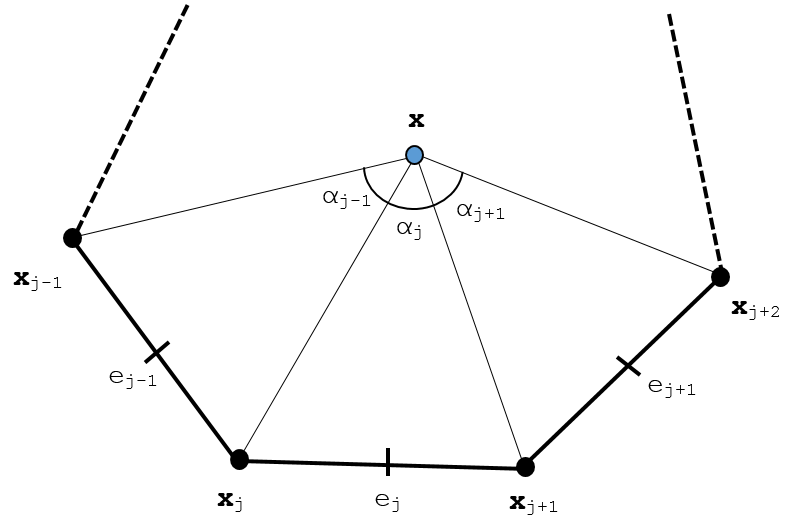
\includegraphics[width=0.65\textwidth]{figures/sec_BF/ref_polygon.png}
\caption{Arbitrary polygon with geometric properties used for 2D basis function generation.}
\label{fig::BF_2D_ref_polygon}
\end{figure}

In this dissertation, all 1st-order, two-dimensional basis functions for a cell will obey the properties for barycentric coordinates. They will form a {\em partition of unity},

\begin{equation}
\sum_{i=1}^{N_K} b_i (\vec{x})  =  1;
\label{eq::BF_linear_interp_partition}
\end{equation}

\noindent coordinate interpolation will result from an {\em affine combination} of the vertices,

\begin{equation}
\sum_{i=1}^{N_K} b_i(\vec{x}) \vec{x}_i  =  \vec{x};
\label{eq::BF_linear_interp_affine}
\end{equation}

\noindent and they will satisfy the {\em Lagrange property},

\begin{equation}
b_i (\vec{x}_j) = \delta_{ij}.
\label{eq::BF_linear_interp_lagrange}
\end{equation}

\noindent $N_K$ is again the number of spatial degrees with measure in element $K$. Using the {\em partition of unity} of Eq. (\ref{eq::BF_linear_interp_partition}), we can rewrite Eqs. (\ref{eq::BF_linear_interp_partition}-\ref{eq::BF_linear_interp_affine}) into a separate, compact, vectorized form for completeness

\begin{equation}
\sum_{i=1}^{N_K}  b_i (\vec{x}) \vec{c}_{i,1}(\vec{x}) = \vec{q}_1 ,
\label{eq::BF_linear_interp_req_vector}
\end{equation}

\noindent where $\vec{c}_{i,1}(\vec{x})$ and $\vec{q}_1$ are the lineary-complete constraint and equivalence terms, respectively. These terms are simply:

\begin{equation}
\vec{c}_{i,1}(\vec{x}) = \left[
\begin{array}{c}
1 \\
x_i - x \\
y_i - y
\end{array} \right]
  \qquad \text{and} \qquad \vec{q}_1 = \left[
\begin{array}{c}
1 \\
0 \\
0
\end{array} \right],
\label{eq::BF_linear_constraint_terms}
\end{equation}

\noindent respectively.

%%%%%%%%%%%%%%%%%%%%%%%%%%%%%%%%%%%%%%%%%%%%%%%%%%%
%%%   SubSection - Linear
\subsection{Linear and BiLinear Basis Functions}
\label{sec::BF_2DLinear_LDandBLD}

Before presenting basis function sets applicable to polytope finite elements, we first provide the two historical basis functions that are exact on triangles and convex quadrilaterals: the $\mathbb{P}_{1}$ and $\mathbb{Q}_{1}$ spaces, respectively.

\begin{equation}
\label{eq::2D_lin_basis_functions}
\begin{aligned}
	b_1(r,s) & = 1-r-s \\
	b_2(r,s) & = r \\
	b_3(r,s) & = s 
\end{aligned}
\end{equation}

\noindent 

and

\begin{equation}
\label{eq::BiL_basis_functions}
\begin{aligned}
	b_1(r,s) & = (1-r)(1-s) \\
	b_2(r,s) & = r(1-s) \\
	b_3(r,s) & = rs \\
	b_4(r,s) & = (1-r)s
\end{aligned}
\end{equation}


%%%%%%%%%%%%%%%%%%%%%%%%%%%%%%%%%%%%%%%%%%%%%%%%%%%
%%%   SubSection - Wachspress
\subsection{Wachspress Rational Basis Functions}
\label{sec::BF_2DLinear_Wachspress}

%%%%%%%%%%%%%%%%%%%%%%%%%%%%%%%%%%%%%%%%%%%%%%%%%%%
%%%   SubSection - Mean Value
\subsection{Mean Value Basis Functions}
\label{sec::BF_2DLinear_MV}


%%%%%%%%%%%%%%%%%%%%%%%%%%%%%%%%%%%%%%%%%%%%%%%%%%%
%%%   SubSection - Maximum Entropy
\subsection{Maximum Entropy Basis Functions}
\label{sec::BF_2DLinear_ME}

%%%%%%%%%%%%%%%%%%%%%%%%%%%%%%%%%%%%%%%%%%%%%%%%%%%
%%%   SubSection - PWL
\subsection{Piecewise Linear (PWL) Basis Functions}
\label{sec::BF_2DLinear_PWL}

\begin{equation}
\label{eq::PWL_2D}
	b_j (x,y) = t_j (x,y) + \alpha_j^K t_c (x,y)
\end{equation}

\noindent $t_j$ is the standard 2D linear function with unity at vertex $j$ that linearly decreases to zero to the cell center and each adjoining vertex. $t_c$ is the 2D cell ``tent'' function which is unity at the cell center and linearly decreases to zero to each cell vertex. $\alpha_{j}^{K}$ is the weight parameter for vertex $j$ in cell $K$. 



%%%%%%%%%%%%%%%
% Begin::2D PWL basis function plots
\pagebreak
\begin{figure}
\label{fig::2D_PWL_unit_square_basis_functions}
\centering
	\begin{subfigure}[b]{0.48\textwidth}
		\centering
		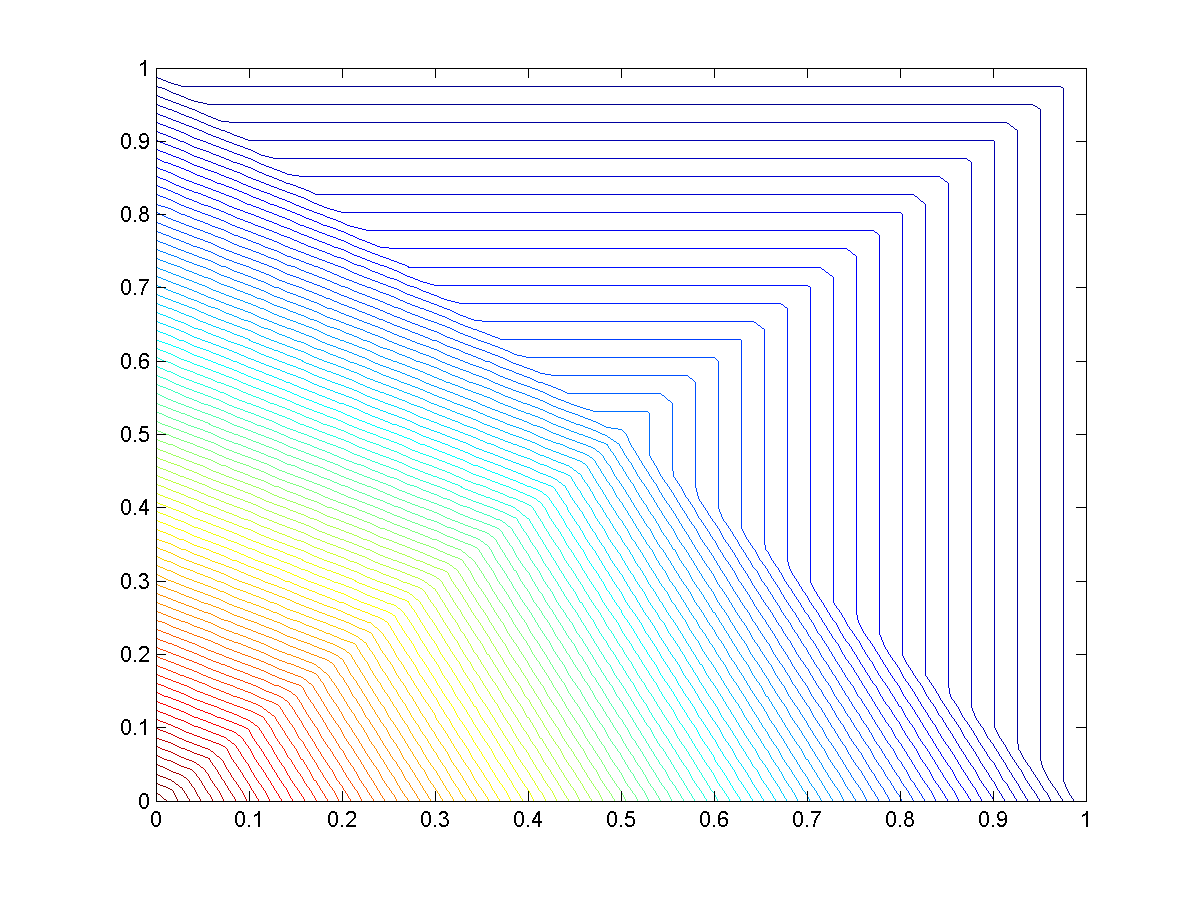
\includegraphics[width=\textwidth]{figures/sec_BF/PWL_square_contour_1.png}
		\caption{}
	\end{subfigure}
	\hfill
	\begin{subfigure}[b]{0.48\textwidth}
		\centering
		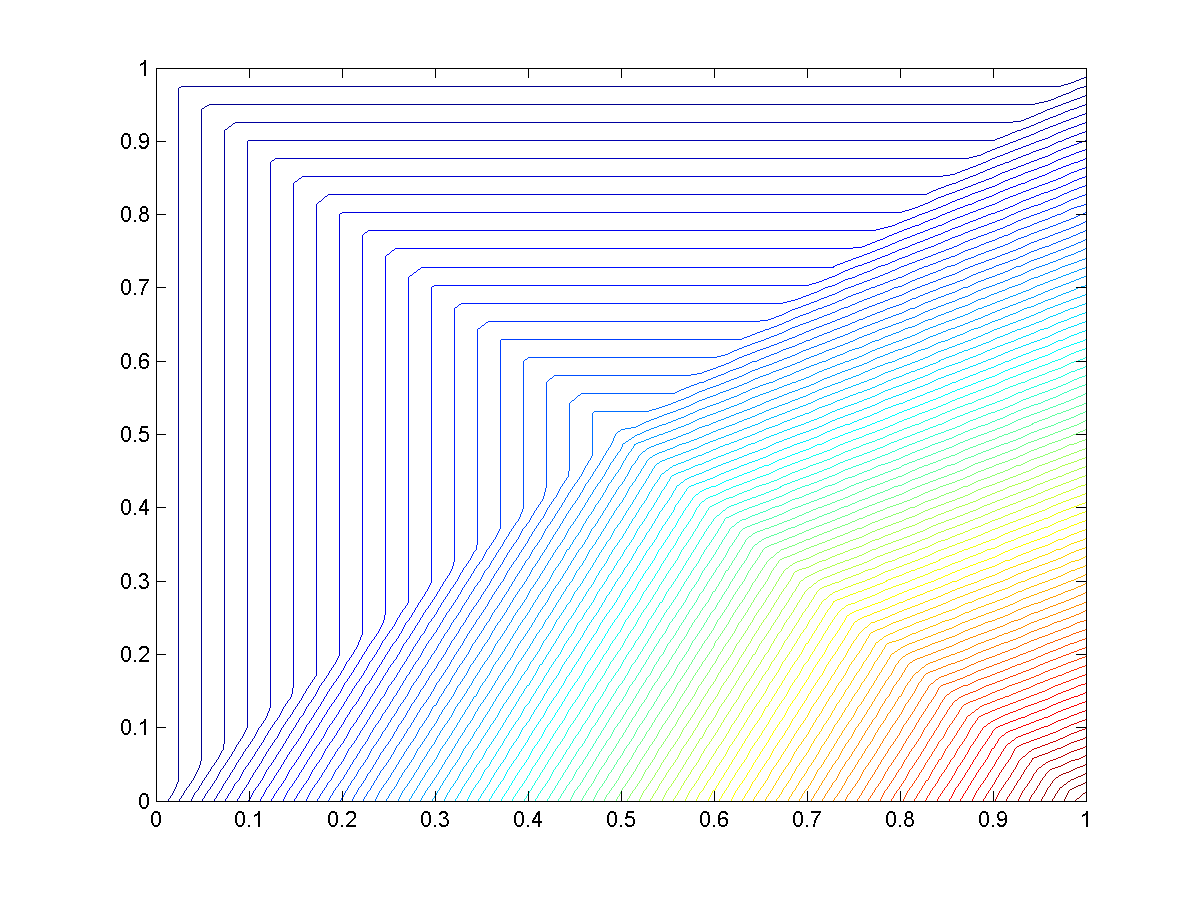
\includegraphics[width=\textwidth]{figures/sec_BF/PWL_square_contour_2.png}
		\caption{}
	\end{subfigure}
	\vfill
	\begin{subfigure}[b]{0.48\textwidth}
		\centering
		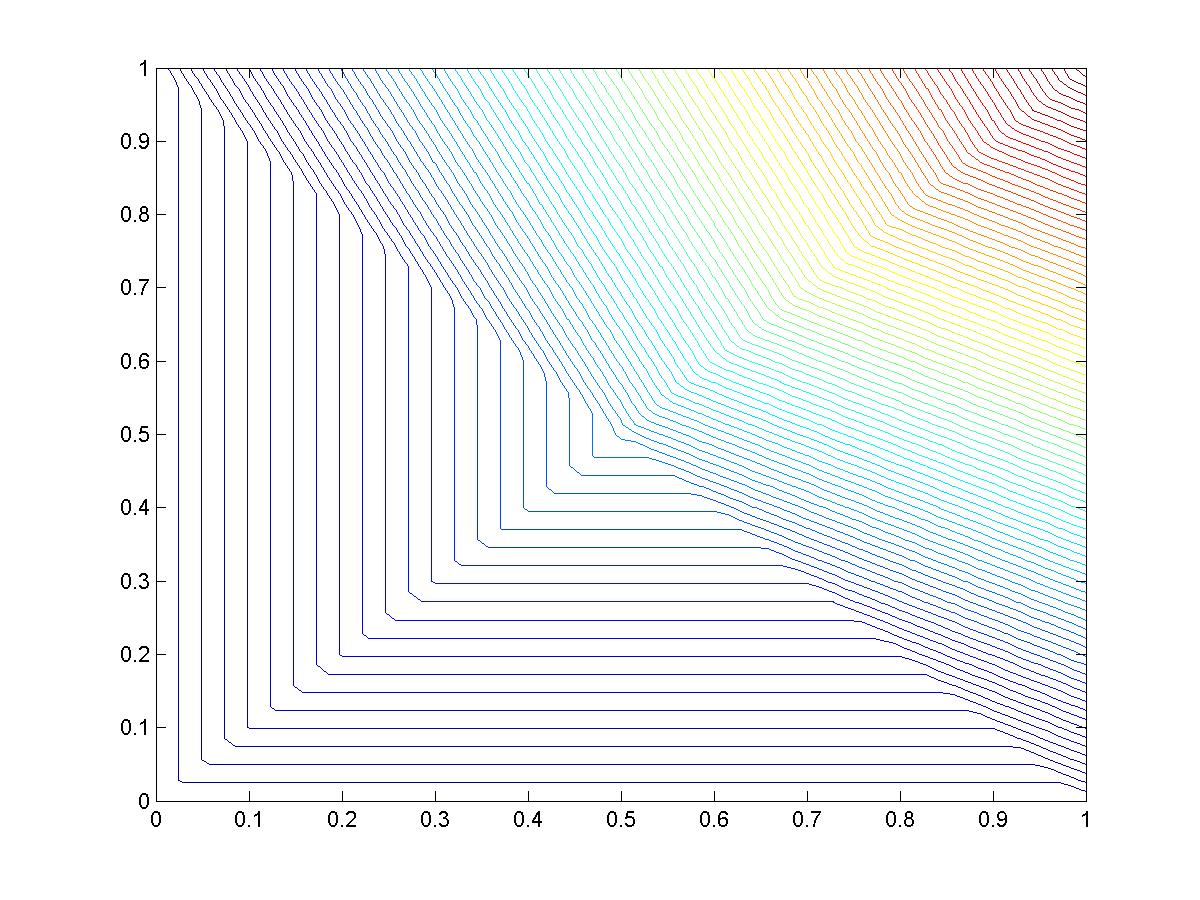
\includegraphics[width=\textwidth]{figures/sec_BF/PWL_square_contour_3.png}
		\caption{}
	\end{subfigure}
	\hfill
	\begin{subfigure}[b]{0.48\textwidth}
		\centering
		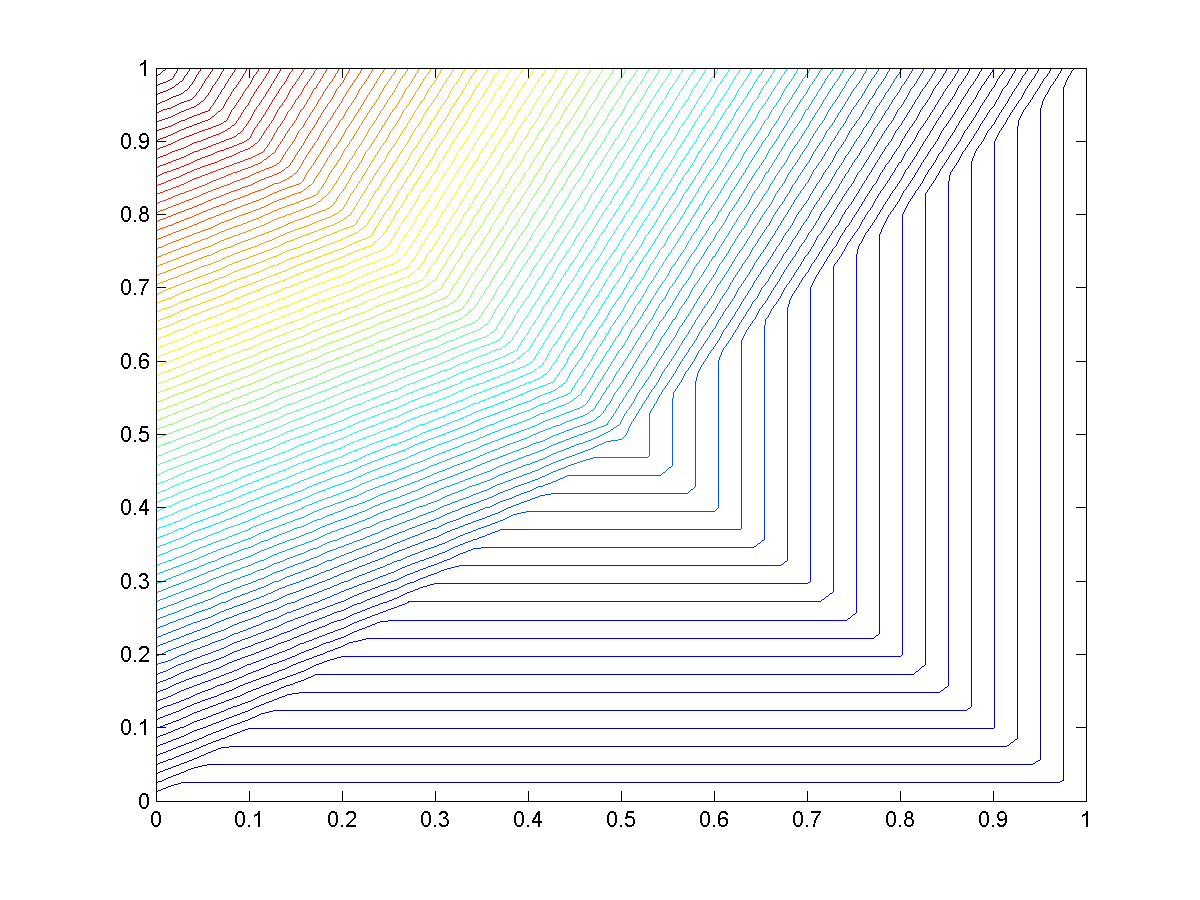
\includegraphics[width=\textwidth]{figures/sec_BF/PWL_square_contour_4.png}
		\caption{}
	\end{subfigure}
\caption{Contour plots of the PWL basis functions on the unit square for the vertices located at: (a) (0,0), (b) (1,0), (c) (1,1), and (d) (0,1).}
\end{figure}

\begin{figure}
\label{fig::2D_pentagon_vertices}
\centering
	\begin{subfigure}[b]{0.40\textwidth}
		\centering
		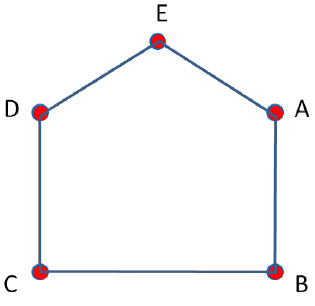
\includegraphics[width=\textwidth]{figures/sec_BF/reg_pent_verts.png}
		\caption{}
	\end{subfigure}
	\hfill
	\begin{subfigure}[b]{0.40\textwidth}
		\centering
		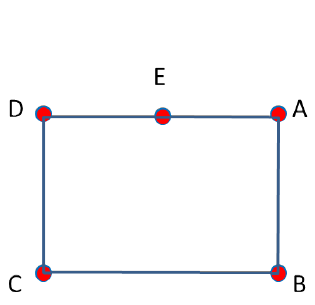
\includegraphics[width=\textwidth]{figures/sec_BF/deg_pent_verts.png}
		\caption{}
	\end{subfigure}
\caption{Vertex structure for a (a) regular pentagonal cell and a (b) degenerate pentagonal cell.}
\end{figure}

\begin{figure}
\label{fig::2D_PWL_pentagon_basis_functions_contour}
\centering
	\begin{subfigure}[b]{0.48\textwidth}
		\centering
		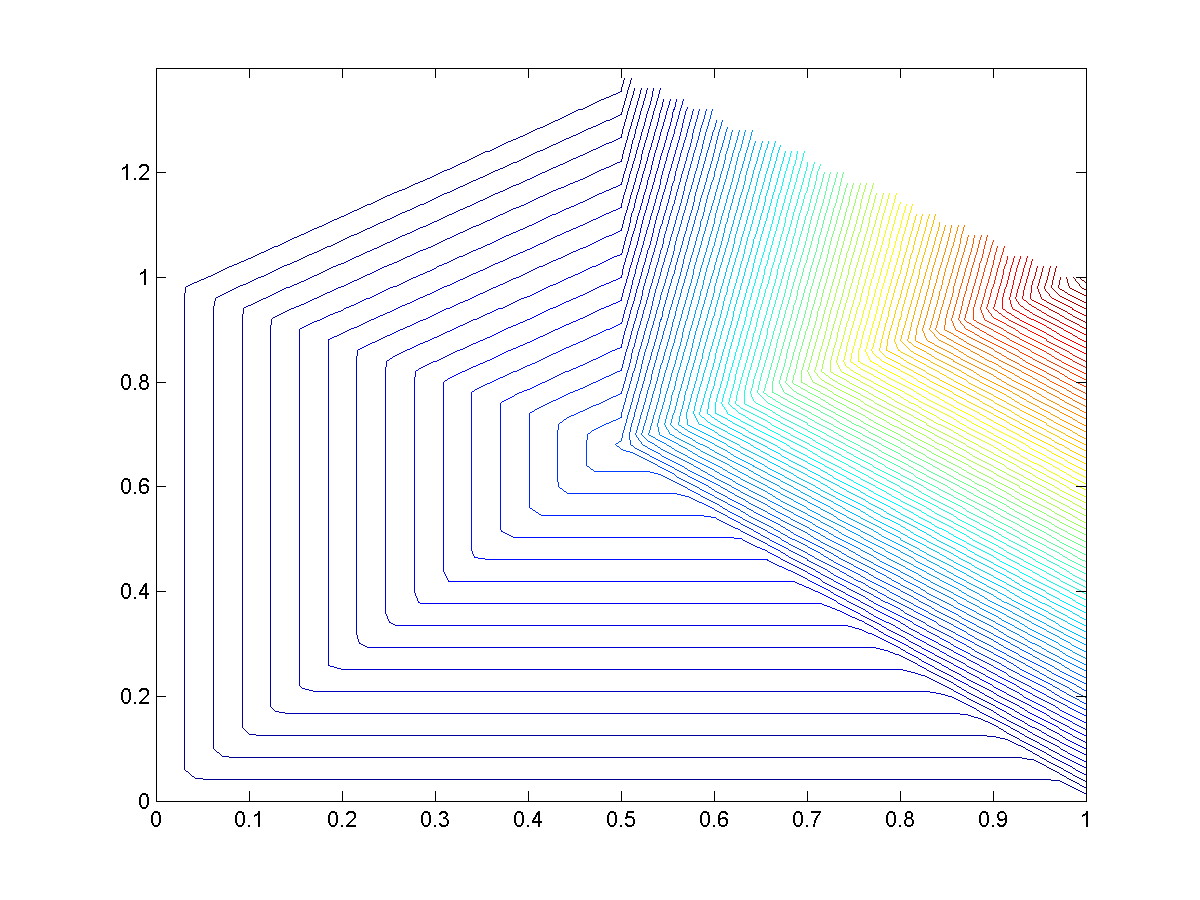
\includegraphics[width=\textwidth]{figures/sec_BF/PWL_rpent_contour_A.png}
		\caption{}
	\end{subfigure}
	\hfill
	\begin{subfigure}[b]{0.48\textwidth}
		\centering
		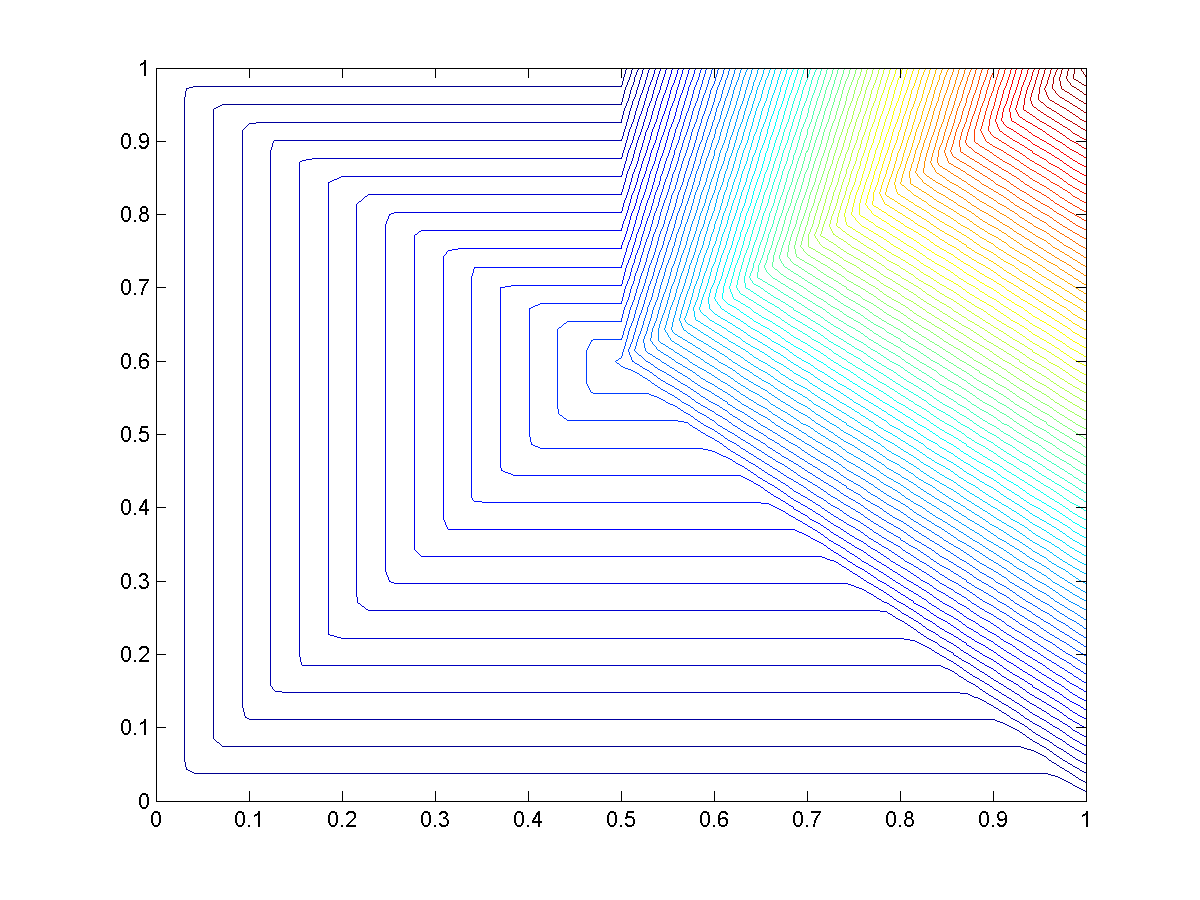
\includegraphics[width=\textwidth]{figures/sec_BF/PWL_dpent_contour_A.png}
		\caption{}
	\end{subfigure}
	\vfill
	\begin{subfigure}[b]{0.48\textwidth}
		\centering
		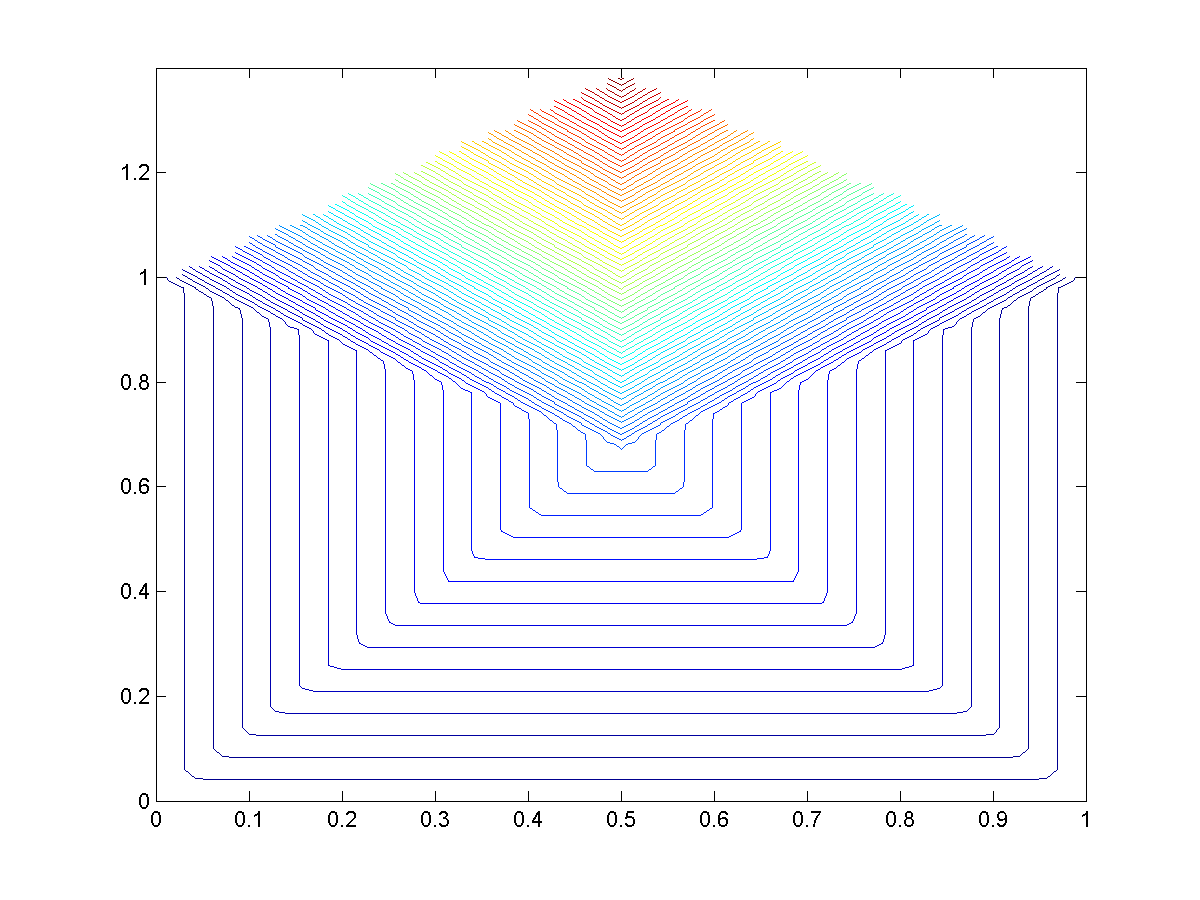
\includegraphics[width=\textwidth]{figures/sec_BF/PWL_rpent_contour_E.png}
		\caption{}
	\end{subfigure}
	\hfill
	\begin{subfigure}[b]{0.48\textwidth}
		\centering
		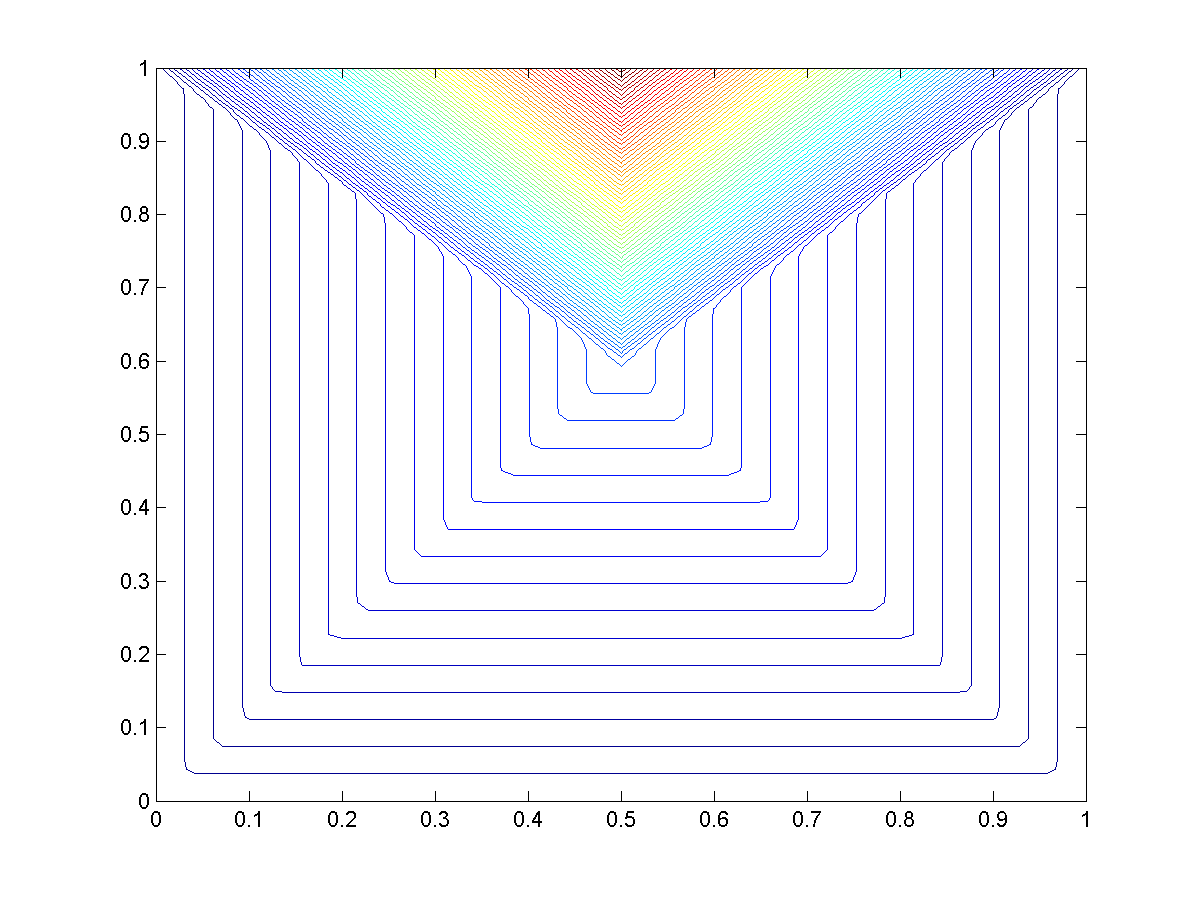
\includegraphics[width=\textwidth]{figures/sec_BF/PWL_dpent_contour_E.png}
		\caption{}
	\end{subfigure}
\caption{Contour plots of the PWL basis functions for a regular pentagon: (a) and (c) as well as a degenerate pentagon: (b) and (d).}
\end{figure}

\begin{figure}
\label{fig::2D_PWL_pentagon_basis_functions_plot}
\centering
	\begin{subfigure}[b]{0.48\textwidth}
		\centering
		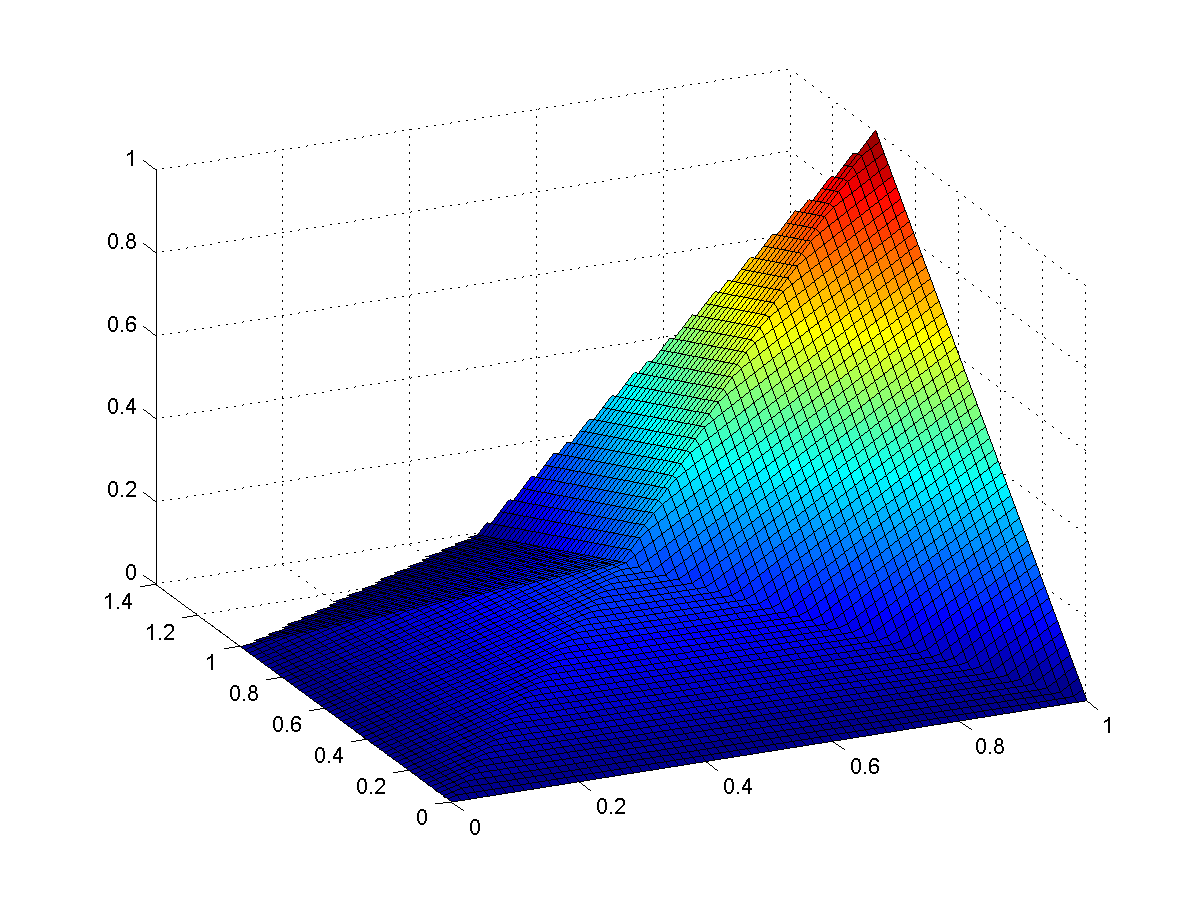
\includegraphics[width=\textwidth]{figures/sec_BF/PWL_rpent_plot_A.png}
		\caption{}
	\end{subfigure}
	\hfill
	\begin{subfigure}[b]{0.48\textwidth}
		\centering
		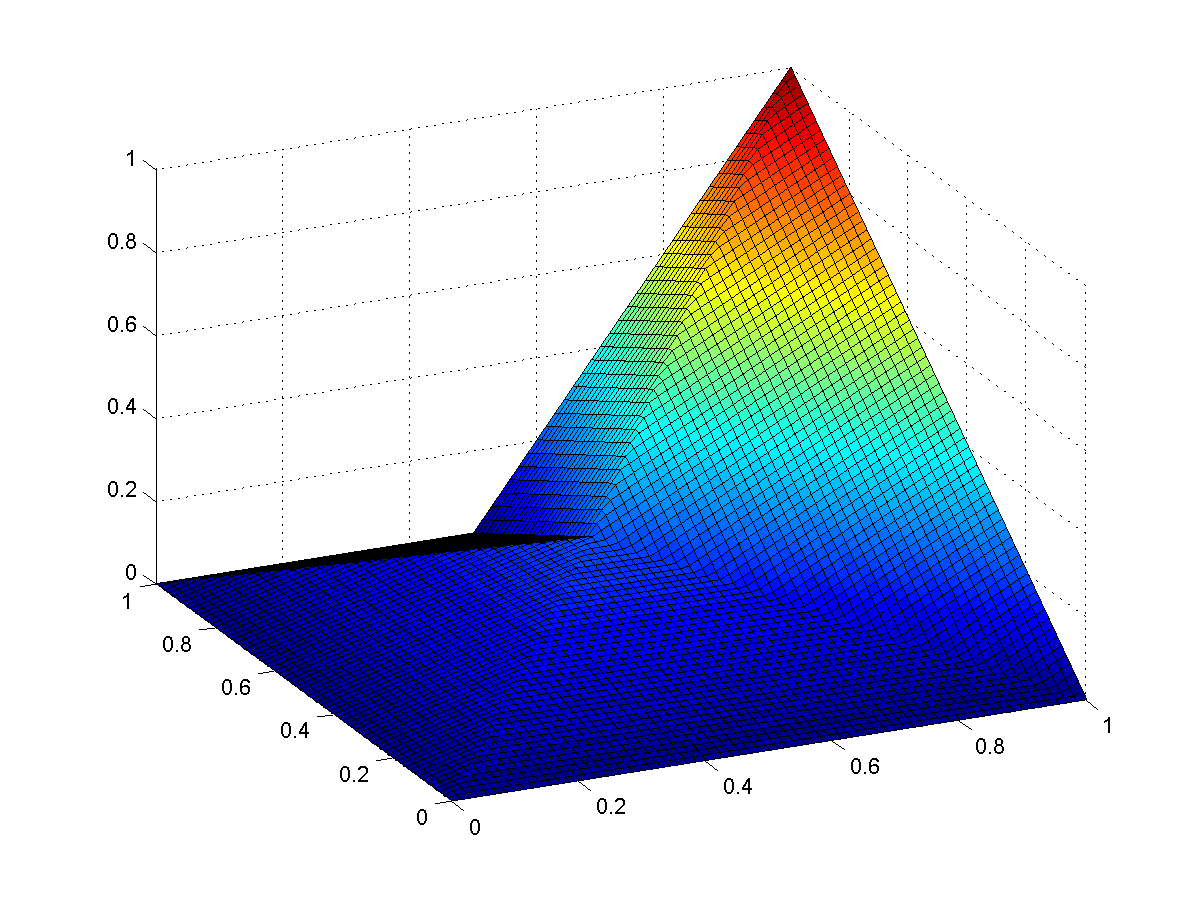
\includegraphics[width=\textwidth]{figures/sec_BF/PWL_dpent_plot_A.png}
		\caption{}
	\end{subfigure}
	\vfill
	\begin{subfigure}[b]{0.48\textwidth}
		\centering
		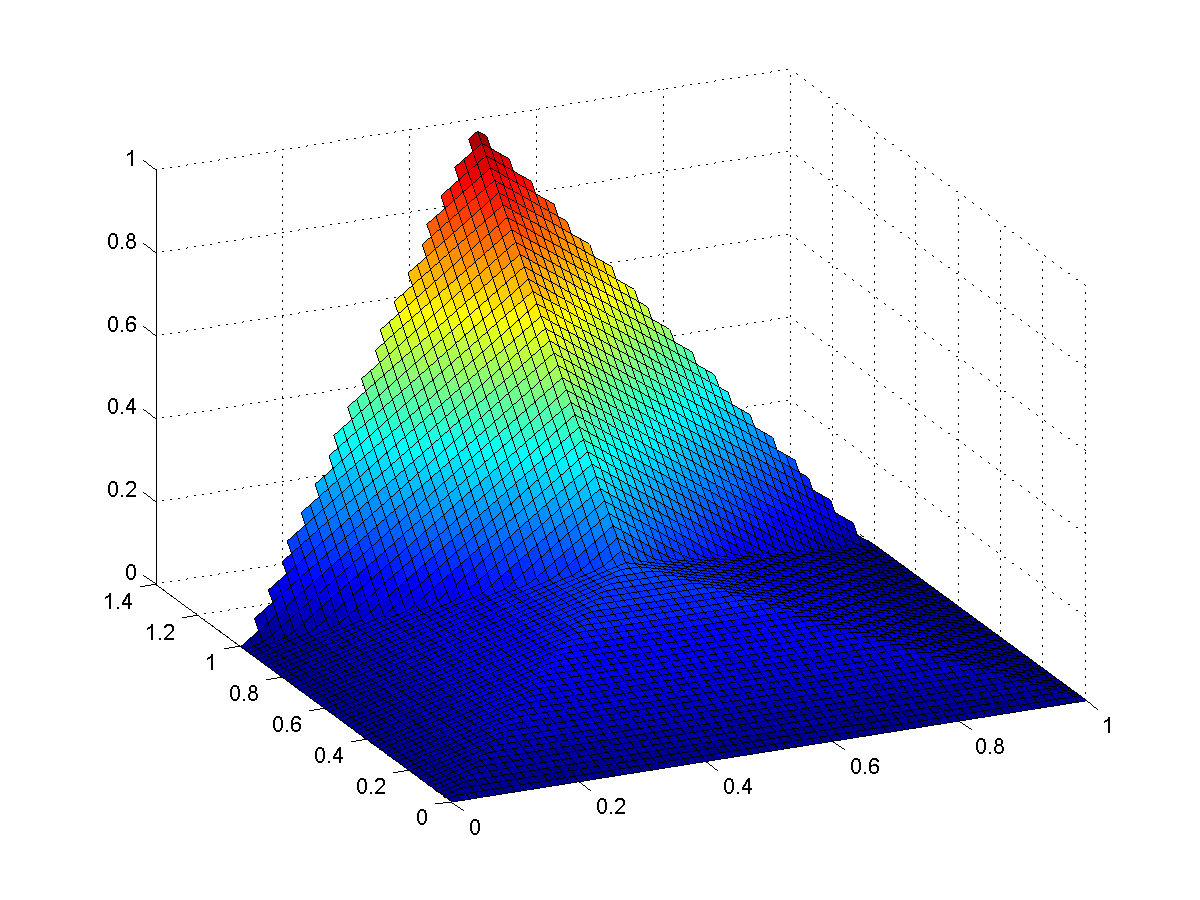
\includegraphics[width=\textwidth]{figures/sec_BF/PWL_rpent_plot_E.png}
		\caption{}
	\end{subfigure}
	\hfill
	\begin{subfigure}[b]{0.48\textwidth}
		\centering
		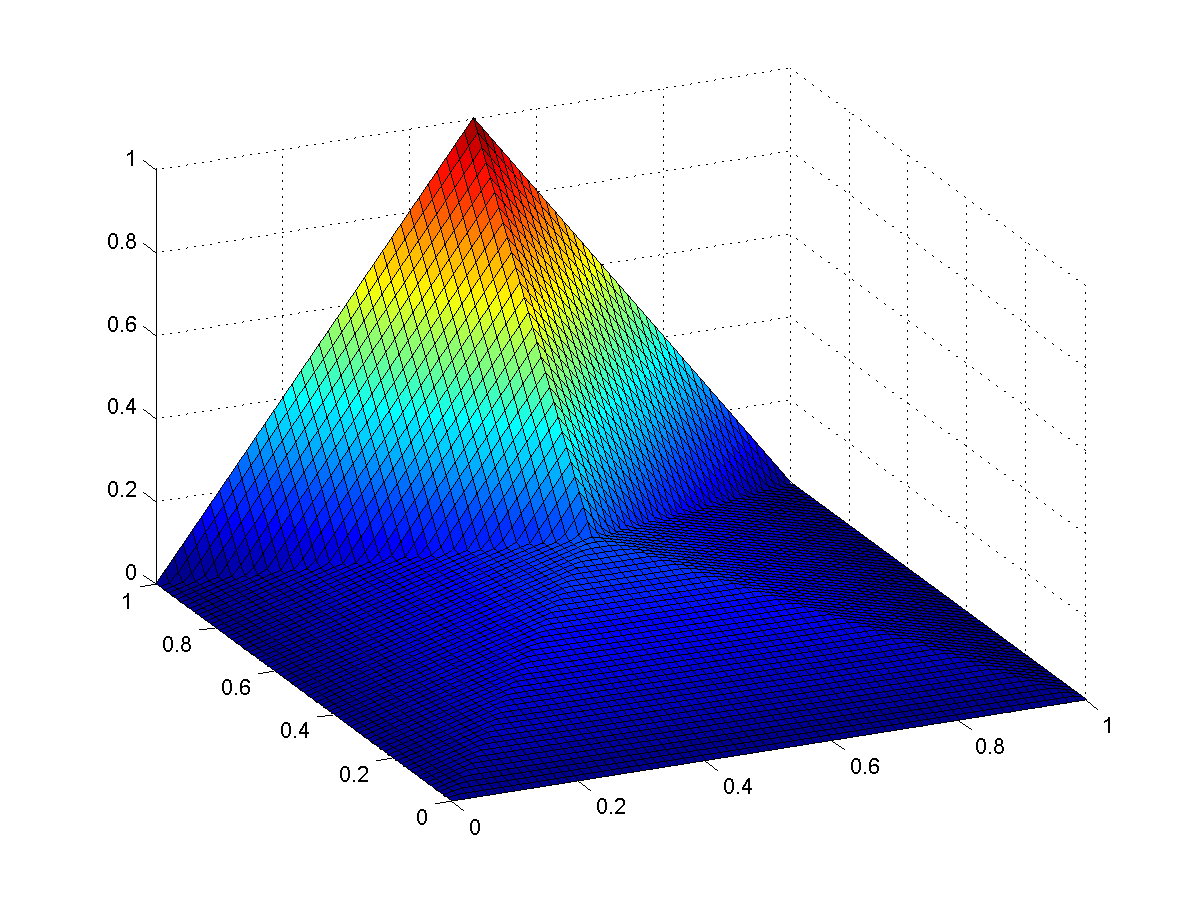
\includegraphics[width=\textwidth]{figures/sec_BF/PWL_dpent_plot_E.png}
		\caption{}
	\end{subfigure}
\caption{Plots of the PWL basis functions for a regular pentagon: (a) and (c) as well as a degenerate pentagon: (b) and (d).}
\end{figure}
% End::2D PWL basis function plots
%%%%%%%%%%%%%%%

%%%%%%%%%%%%%%%%%%%%%%%%%%%%%%%%%%%%%%%%%%%%%%%%%%%
%%%   SubSubSection - 2D linear summary
\subsection{Summary of 2D Linear Basis Functions on Polygons}
\label{sec::BF_2DLinear_Summary}

%%%%%%%%%%%%%%%%%%%%%%%%%%%%%%%%%%%%%%%%%%%%%%%%%%%
%%%   Section - Quadratic Basis Functions
\section{Quadratic Serendipity Basis Functions on 2D Polygons}
\label{sec::BF_2DQuadratic}

\begin{gather}
	 \sum_{i=1}^{N_K} b_i (\vec{x})  =  1 \\
	\sum_{i=1}^{N_K} b_i(\vec{x}) \vec{x}_i  =  \vec{x} \\
	\sum_{i=1}^{N_K} \sum_{j=1}^{N_K} \mu _{i,j}  \left(   \frac{\vec{x}_i \otimes \vec{x}_j +\vec{x}_j \otimes \vec{x}_i }{2}  \right)  = \vec{x} \otimes \vec{x}
\label{eq::quadratic_interp_requirements}
\end{gather}

\noindent where $\mu_{i,j}$ is a weight function corresponding to particular basis function pairings.

%%%%%%%%%%%%%%%%%%%%%%%%%%%%%%%%%%%%%%%%%%%%%%%%%%%
%%%   Section - 3D
\section{Linear Basis Functions on 3D Polyhedra}
\label{sec::BF_3DLinear}



%%%%%%%%%%%%%%%%%%%%%%%%%%%%%%%%%%%%%%%%%%%%%%%%%%%
%%%   SubSection - 3D Lin/TriL
\subsection{3D Linear and TriLinear Basis Functions}
\label{sec::BF_3DLinear_TriL}

\begin{figure}
\centering
	\begin{subfigure}[b]{0.45\textwidth}
		\centering
		\label{subfig::unit_square}
		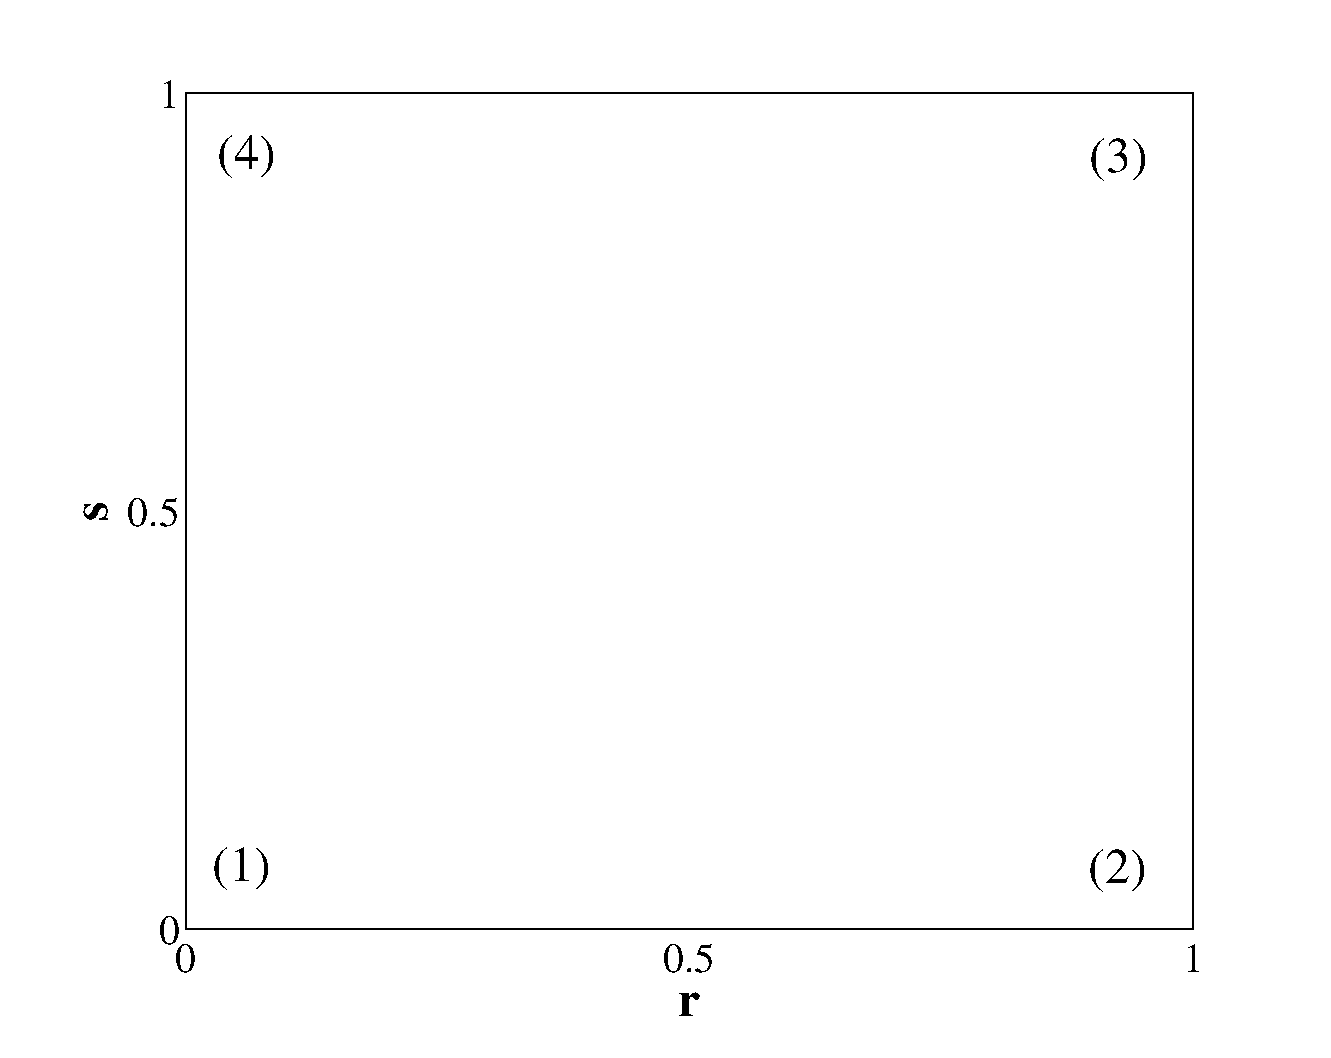
\includegraphics[width=\textwidth]{figures/sec_BF/unit_square_linear.eps}
		\caption{}
	\end{subfigure}
	\hfill
	\begin{subfigure}[b]{0.45\textwidth}
		\centering
		\label{subfig::unit_cube}
		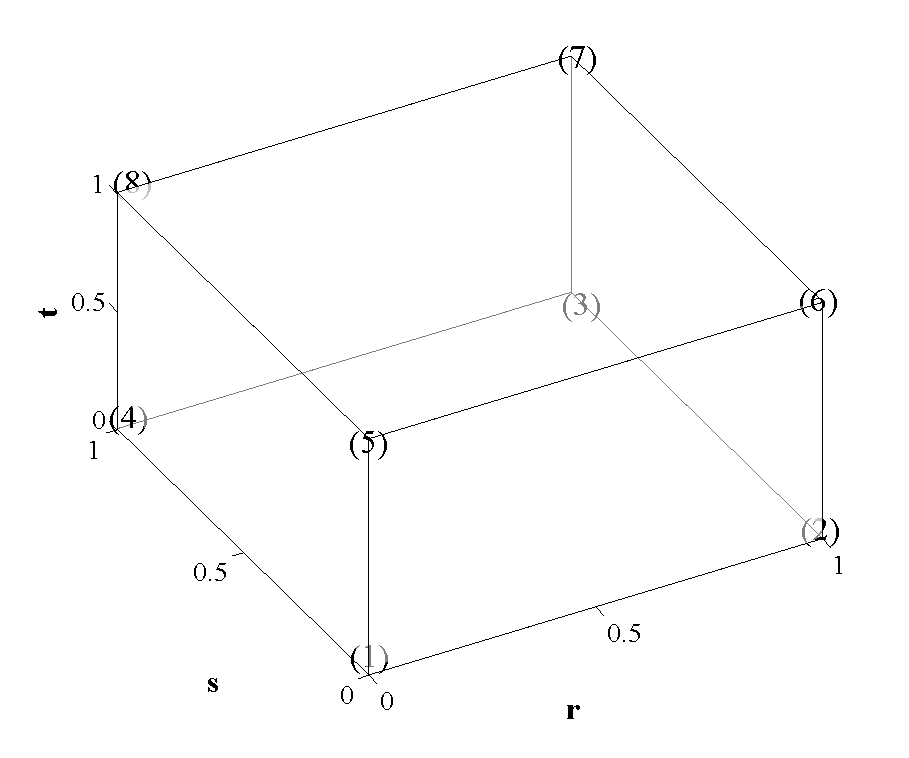
\includegraphics[width=\textwidth]{figures/sec_BF/unit_cube_linear.eps}
		\caption{}
	\end{subfigure}
\caption{Vertex structure for the (a) unit square and (b) unit cube.}
\label{fig::BF_3D_unit_tet_cube}
\end{figure}

\begin{equation}
\label{eq::3D_lin_basis_functions}
\begin{aligned}
	b_1(r,s) & = 1-r-s-t \\
	b_2(r,s) & = r \\
	b_3(r,s) & = s \\
	b_4(r,s) & = t
\end{aligned}
\end{equation}

\noindent and

\begin{equation}
\label{eq::TriL_basis_functions}
\begin{aligned}
	b_1(r,s,t) & = (1-r)(1-s)(1-t) \\
	b_2(r,s,t) & = r(1-s)(1-t) \\
	b_3(r,s,t) & = rs(1-t) \\
	b_4(r,s,t) & = (1-r)s(1-t) \\
	b_5(r,s,t) & = (1-r)(1-s)t \\
	b_6(r,s,t) & = r(1-s)t \\
	b_7(r,s,t) & = rst \\
	b_8(r,s,t) & = (1-r)st \\
\end{aligned}
\end{equation}

%%%%%%%%%%%%%%%%%%%%%%%%%%%%%%%%%%%%%%%%%%%%%%%%%%%
%%%   SubSection - PWL
\subsection{3D Piecewise Linear (PWL) Basis Functions}
\label{sec::BF_3DLinear_PWL}

The 3D PWL basis functions share a similar form to the 2D PWL basis functions.

\begin{equation}
\label{eq::PWL_3D}
	b_j (x,y,z)  = t_j  (x,y,z) + \sum_{f=1}^{F_j} \beta_f^j  t_f (x,y,z) + \alpha_j^K t_c  (x,y,z)
\end{equation}

\noindent $t_j$ is the standard 3D linear function with unity at vertex $j$ that linearly decreases to zero to the cell center, the face center for each face that includes vertex $j$, and each vertex that shares an edge with vertex $j$. $t_c$ is the 3D cell ``tent" function which is unity at the cell center and linearly decreases to zero to each cell vertex and face center. $t_f$ is the face "tent" function which is unity at the face center and linearly decreases to zero at each vertex on that face and the cell center. $\beta_{f,j}$ is the weight parameter for face $f$ touching cell vertex $j$, and $F_j$ is the number of faces touching vertex $j$. Like the previous work defining the PWLD method \cite{bailey2008phd}, we also choose to assume the cell and face weighting parameters are

\begin{equation}
\alpha_{K,j} = \frac{1}{N_K} \qquad \text{and} \qquad \beta_{f,j} = \frac{1}{N_f},
\label{eq::PWL_weight_vals}
\end{equation}

\noindent respectively, where $N_K$ is the number of vertices in cell $K$ and $N_f$ is the number of vertices on face $f$, which leads to constant values of $\alpha$ and $\beta$ for each cell and face, respectively. This assumption of the cell weight function holds for both 2D and 3D.

%%%%%%%%%%%%%%%%%%%%%%%%%%%%%%%%%%%%%%%%%%%%%%%%%%%
%%%   Section - Results
\section{Numerical Results}
\label{sec::BF_Results}

Now that we have presented several linear polygonal finite element basis sets along with the methodology to convert them to quadratic serendipity-like basis, we present several numerical problems to demonstrate our methodology. First, we demonstrate that the presented basis sets can capture an exactly-linear transport solution in Section \ref{sec::BF_Results_Linear}. Next, we present some convergence properties of the basis sets using the method of manufactured solutions (MMS) in Section \ref{sec::BF_Results_MMS}. We then present a searchlight problem and observe how the basis sets react with adaptive mesh refinement (AMR) to mitigate numerical dispersion through a vacuum in Section \ref{sec::BF_Results_SL}.

%%%%%%%%%%%%%%%%%%%%%%%%%%%%%%%%%%%%%%%%%%%%%%%%%%%
%%%   SubSection - Linear Solutions = METHOD OF EXACT SOLUTIONS
\subsection{Two-Dimensional Exactly-Linear Transport Solutions}
\label{sec::BF_Results_Linear}

We present our first numerical example by demonstrating that the linear and quadratic polygonal finite element basis functions capture an exactly-linear solution space. We will show this by the method of exact solutions (MES). Since the coordinate interpolation of the basis functions for the linear basis functions requires exact linear interpolation (Eq. (\ref{eq::BF_linear_interp_affine})), then an exactly-linear solution space can be captured, even on highly distorted polygonal meshes. This also applies to the quadratic serendipity space since it is formed by the product-wise pairings of the linear basis functions. We build our exact solution by investigating the 2D, 1 energy group transport problem with no scattering and an angle-dependent distributed source,

\begin{equation}
\label{eq::BF_Results_Linear_angflux}
\mu \frac{\partial \Psi}{\partial x} + \eta \frac{\partial \Psi}{\partial y} + \sigma_t \Psi = Q(x,y, \mu, \eta), 
\end{equation}

\noindent where the streaming term was separated into the corresponding two-dimensional terms. We chose to drop the scattering term for this example so that the error arising from iteratively converging our solution would have no impact.

We then define an angular flux solution that is linear in both space and angle along with the corresponding 0th moment scalar flux solution:

\begin{equation}
\label{eq::BF_Results_Linear_fluxsols}
\begin{aligned}
\Psi (x,y,\mu,\eta) &= ax + by + c \mu + d\eta + e\\
\Phi (x,y) &= 2 \pi \left( ax + by  + e \right)
\end{aligned} .
\end{equation}

\noindent One can immediately notice that our 0th moment solution is not dependent on angle. We arrive at this solution by enforcing our 2D angular quadrature set to have the following properties:

\begin{equation}
\label{eq::BF_Results_Linear_quadrules}
\sum_{q} w_q = 2 \pi \qquad \text{and} \qquad \sum_{q} w_q  \left[
	\begin{array}{c}
		\mu_q \\
		\eta_q
	\end{array} \right] = \left[
	\begin{array}{c}
		0 \\
		0
	\end{array} \right] .
\end{equation}

Our boundary conditions for all inflow boundaries are then uniquely determined by the angular flux solution of Eq. (\ref{eq::BF_Results_Linear_fluxsols}). Inserting the angular flux solution of Eq. (\ref{eq::BF_Results_Linear_fluxsols}) into Eq. (\ref{eq::BF_Results_Linear_angflux}), we obtain the distributed source that will produce our exactly-linear solution space:

\begin{equation}
\label{eq::BF_Results_Linear_src}
Q(x,y,\mu,\eta) = a \mu + b \eta + \sigma_t \left(  c \mu + d \eta \right) + \sigma_t \left( ax +by + e   \right).
\end{equation}

\noindent It is noted that the angular dependence of the source can be removed (which can ease the code development burden) if one sets

\begin{equation}
\label{eq::BF_Results_Linear_removeterms}
\begin{aligned}
	a &= - c \, \sigma_t, \\
	b &= - d \, \sigma_t.
\end{aligned}
\end{equation}

For this example, we test the various 2D polygonal finite element basis functions on six different mesh types. These mesh types include triangular, quadrilateral, and polygonal meshes:

\begin{enumerate}
	\item Orthogonal cartesian mesh formed by the intersection of 11 equally-spaced vertices in both the $x$ and $y$ dimensions. This forms a 10x10 array of quadrilateral mesh cells.
	\item Ordered-triangular mesh formed by the bisection of the previous orthogonal cartesian mesh (forming 200 triangles all of the same size/shape).
	\item Quadrilateral shestakov grid formed by the randomization of vertices based on a skewness parameter \cite{shestakov1988solution,shestakov1990test}. With a certain range of this skewness parameter, highly distorted meshes can be generated.
	\item Sinusoidal polygonal grid that is generated by the transformation of a uniform orthogonal grid based on a sinusoid functional. The transformed vertices are then converted into a polygonal grid by computing a bounded Voronoi diagram.
	\item Kershaw's quadrilateral z-mesh \cite{kershaw1981differencing}. This mesh is formed by taking an orthogonal quadrilateral grid and displacing certain interior vertices only in the $y$ dimension.
	\item A polygonal variant of the quadrilateral z-mesh. The polygonal grid is formed in a similar manner to the sinusoidal polygonal mesh with a Voronoi diagram.
\end{enumerate}

\noindent We also wish that both the angular flux solution as well as the 0th moment solution are strictly positive everywhere. Therefore, we set the function parameters in Eq. (\ref{eq::BF_Results_Linear_fluxsols}) to $\sigma_t = a = c = d = e = 1.0$ and $b = 1.5$. We gave the solution the $40 \%$ tilt in space ($a \neq b$) so that it would not align with the triangular mesh. Using an S8 LS quadrature set, we ran all combinations of the polygonal basis functions and the mesh types. The linear solutions for the Wachspress, PWL, mean value, linear maximum entropy, and quadratic serendipity maximum entropy basis functions are presented in Figures \ref{fig::BF_Results_Linear_wach_sol}, \ref{fig::BF_Results_Linear_pwld_sol}, \ref{fig::BF_Results_Linear_mv_sol}, \ref{fig::BF_Results_Linear_me1_sol}, and \ref{fig::BF_Results_Linear_me2_sol}, respectively. We can see that for all the polygonal basis functions, an exact linear solution is captured as shown by the unbroken nature of the contour lines. This even holds on the highly distorted quadrilateral shestakov mesh.

%%%%%%%%%%%%%%%%%
% Begin Linear Solution figures
\begin{figure}
\centering
	\begin{subfigure}[b]{0.45\textwidth}
		\centering
		\label{subfig::cart_wach_lin_sol}
		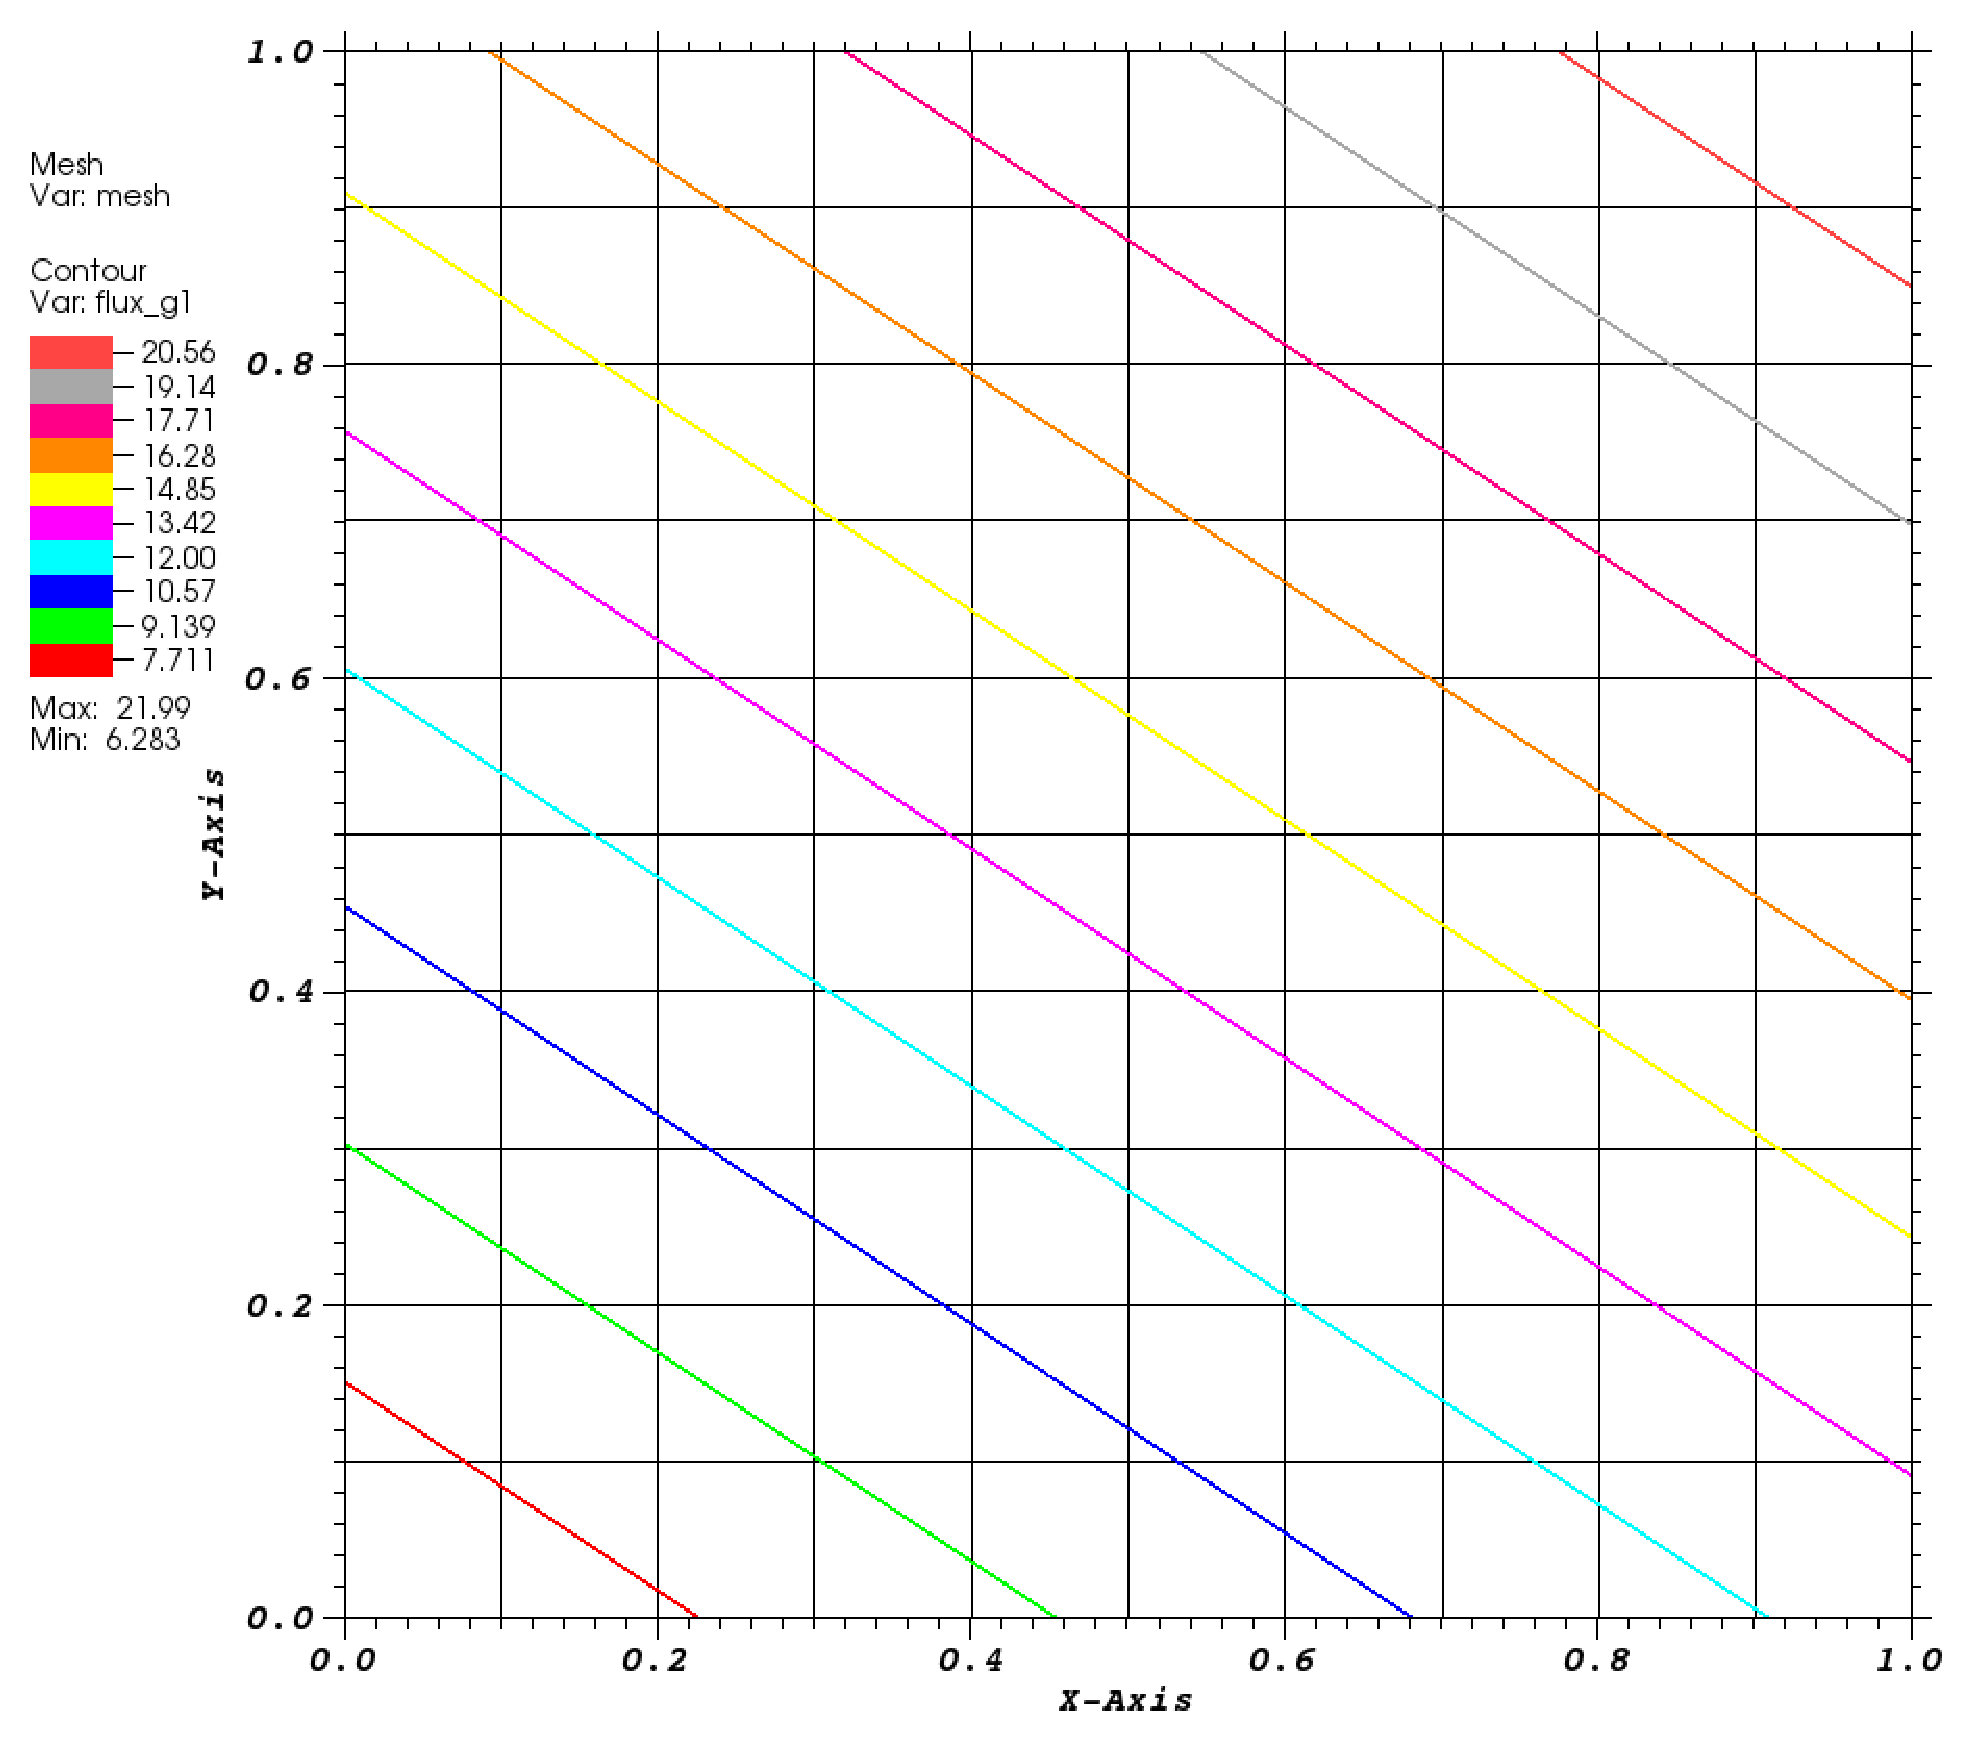
\includegraphics[width=\textwidth]{figures/sec_BF/cart_WACHSPRESS_k1.eps}
		\caption{}
	\end{subfigure}
	\hfill
	\begin{subfigure}[b]{0.45\textwidth}
		\centering
		\label{subfig::tri_wach_lin_sol}
		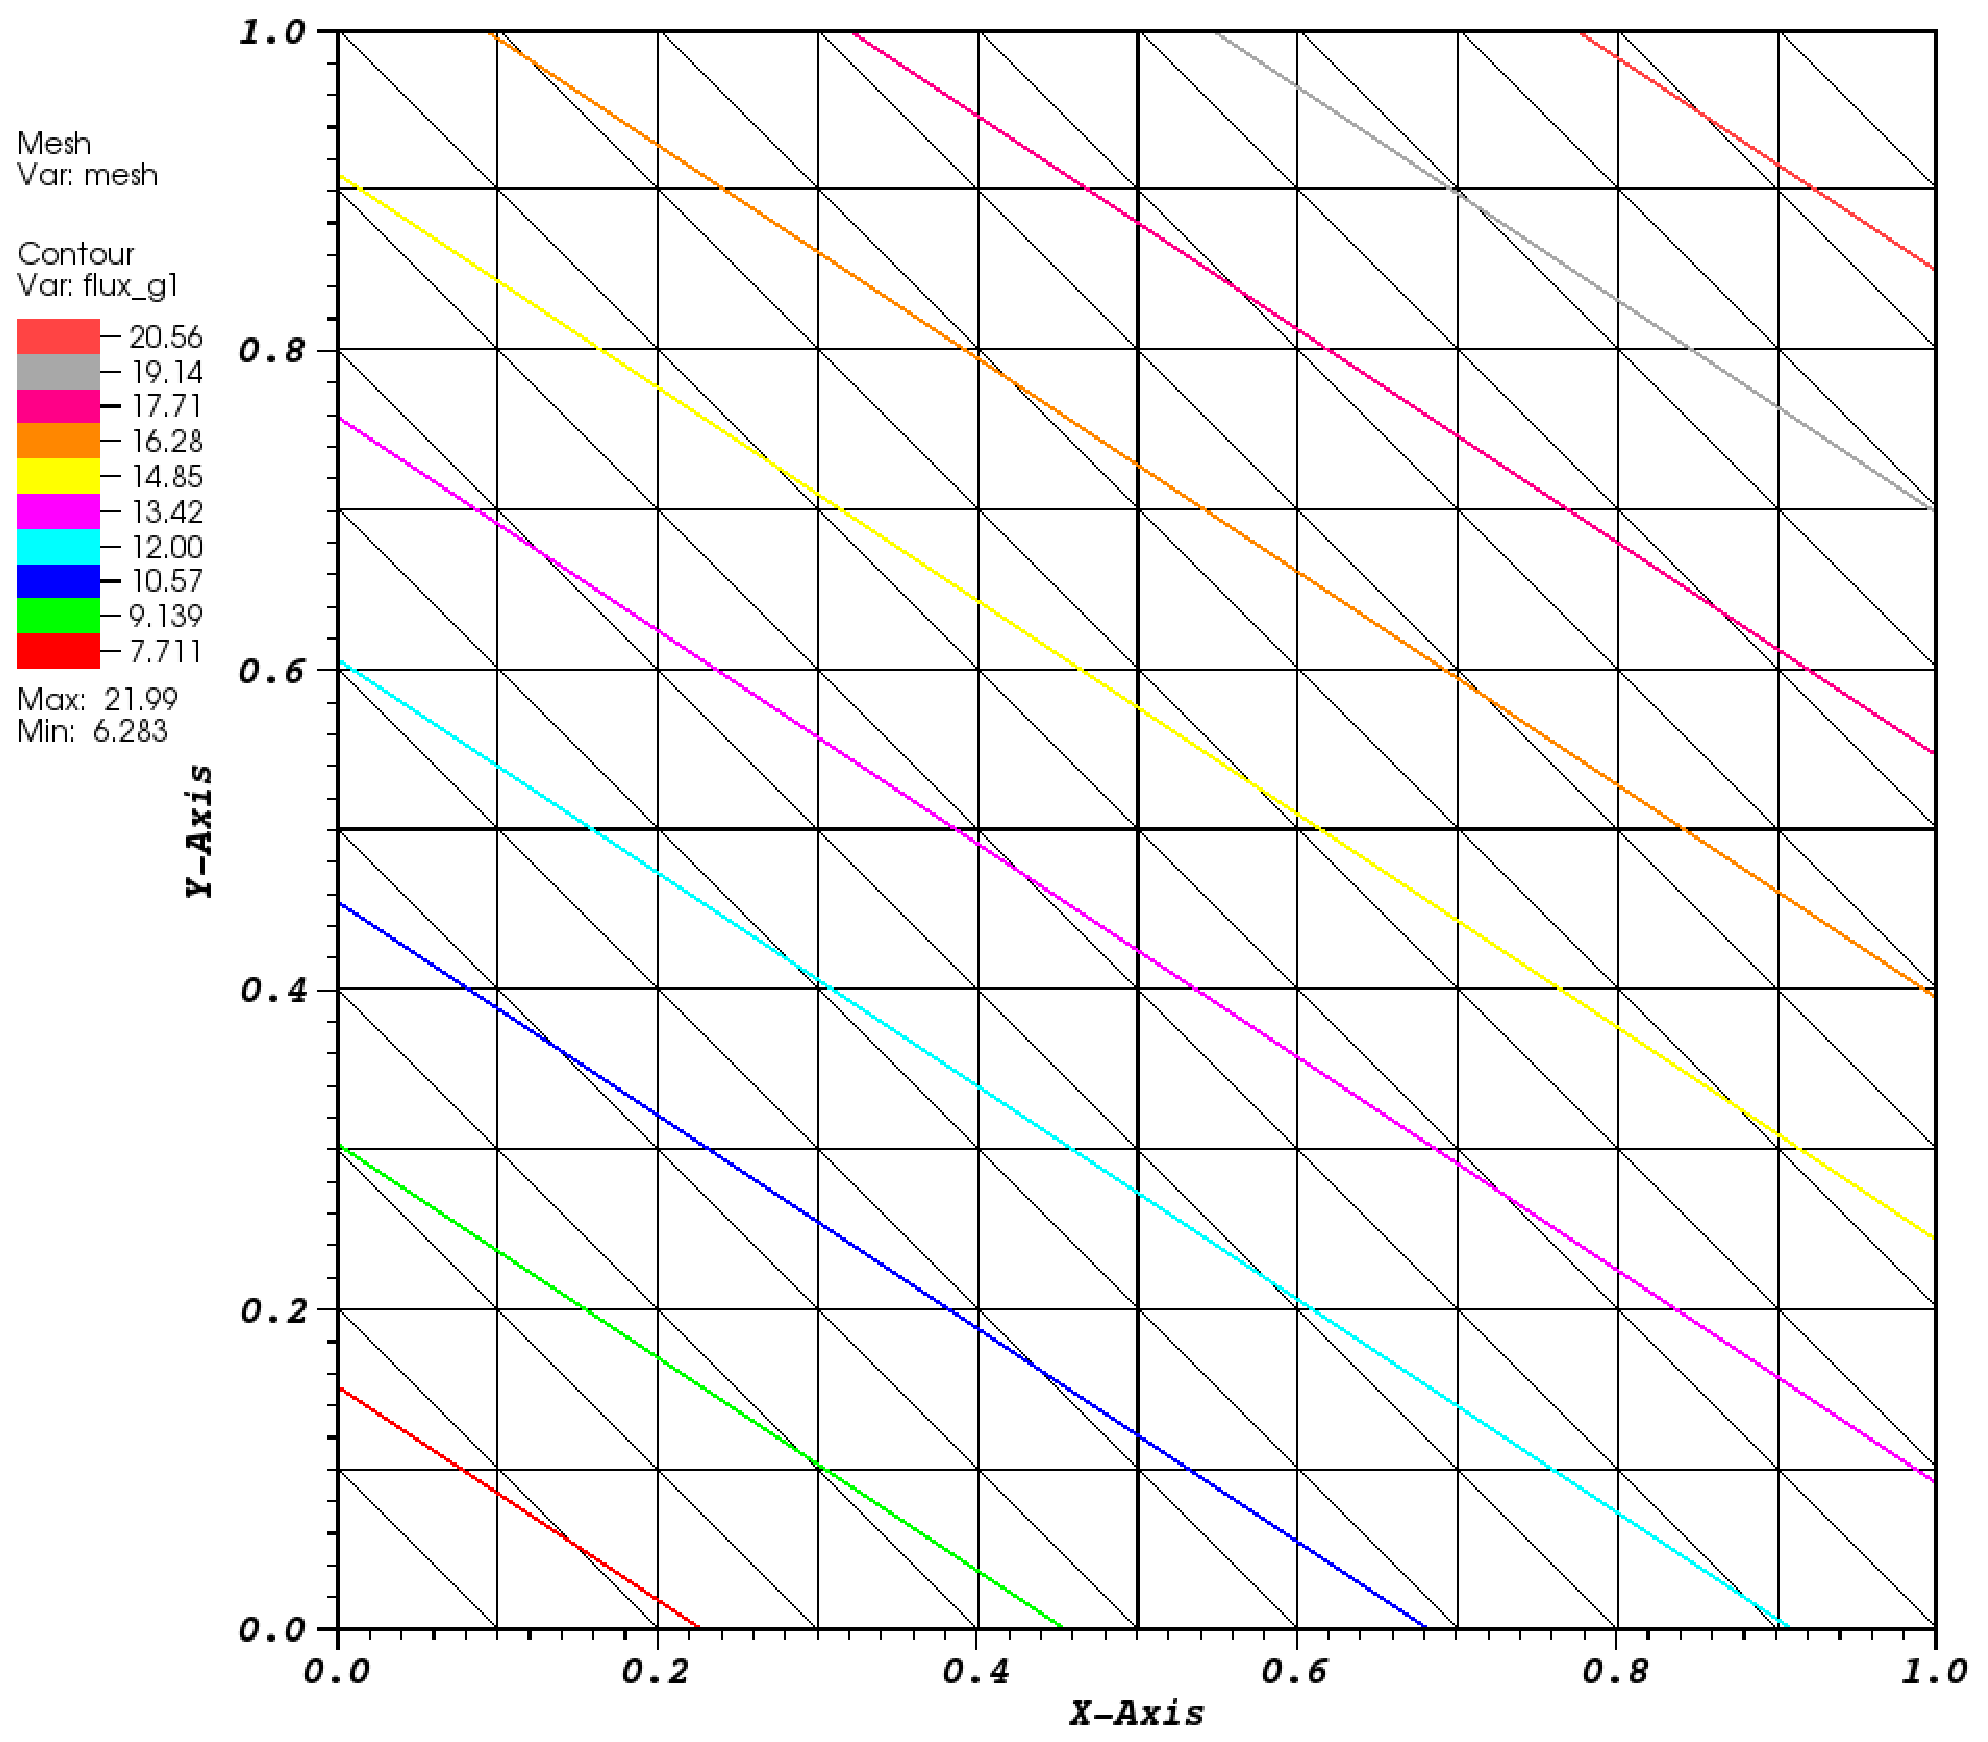
\includegraphics[width=\textwidth]{figures/sec_BF/tri_WACHSPRESS_k1.eps}
		\caption{}
	\end{subfigure}
	\vfill
	\begin{subfigure}[b]{0.45\textwidth}
		\centering
		\label{subfig::shes_quad_wach_lin_sol}
		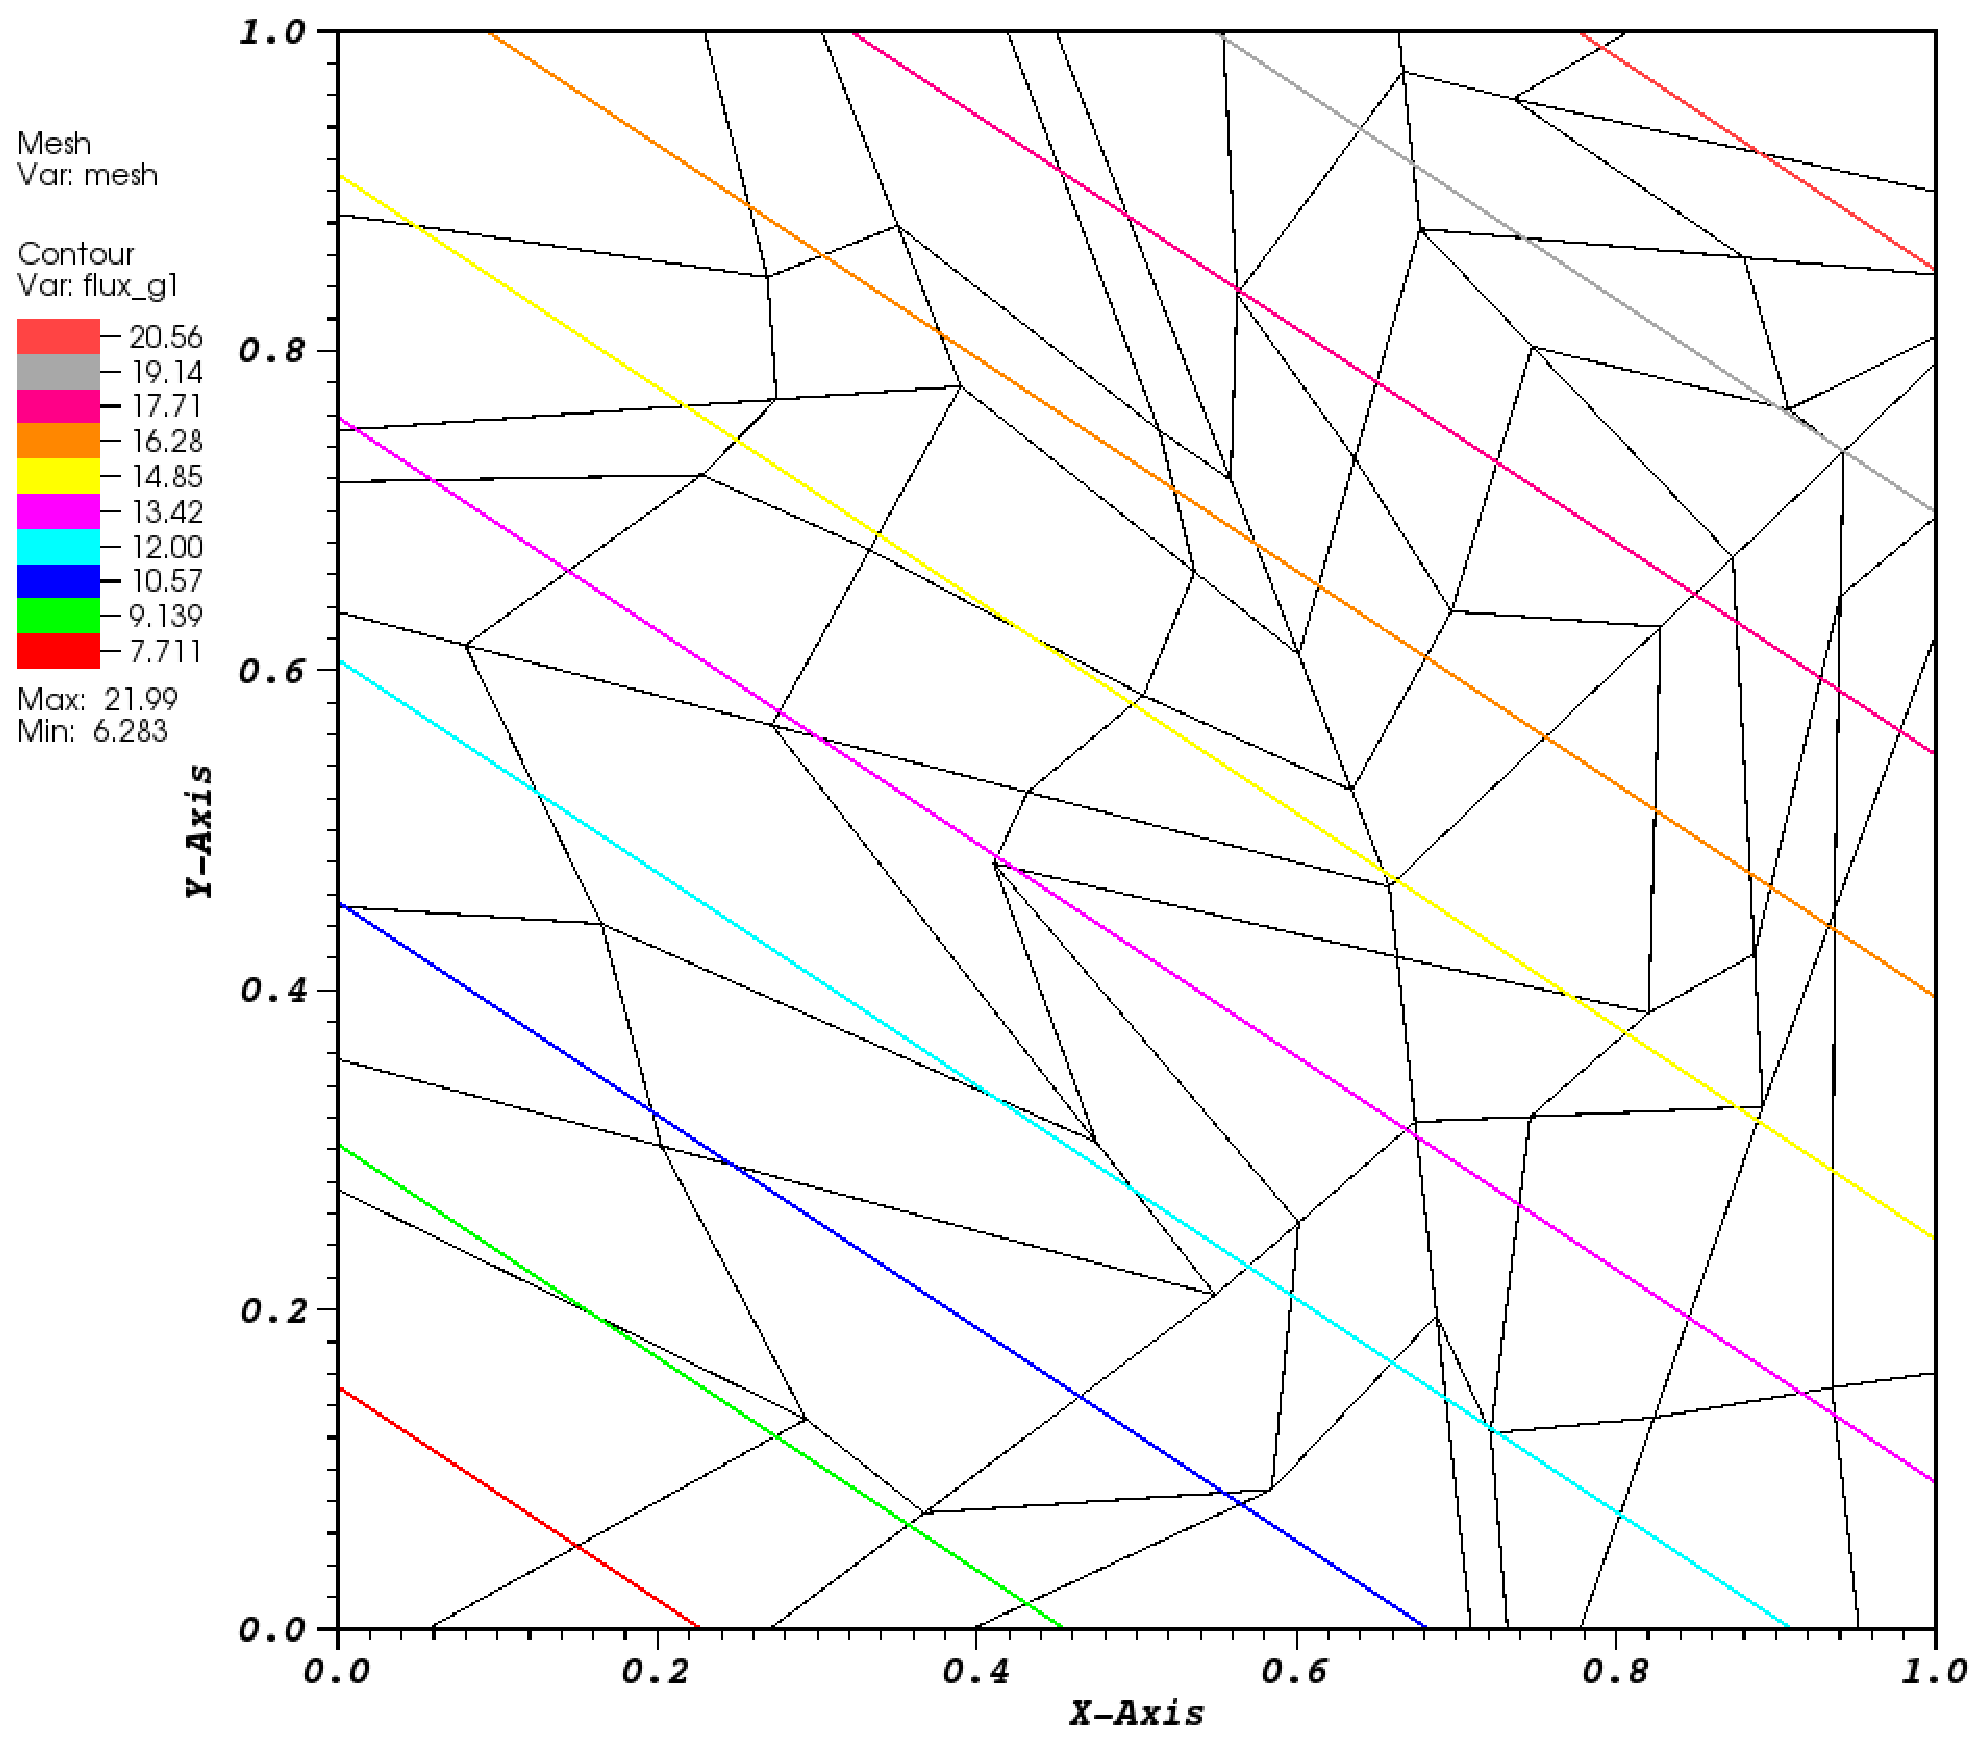
\includegraphics[width=\textwidth]{figures/sec_BF/shes_quad_WACHSPRESS_k1.eps}
		\caption{}
	\end{subfigure}
	\hfill
	\begin{subfigure}[b]{0.45\textwidth}
		\centering
		\label{subfig::smooth_poly_wach_lin_sol}
		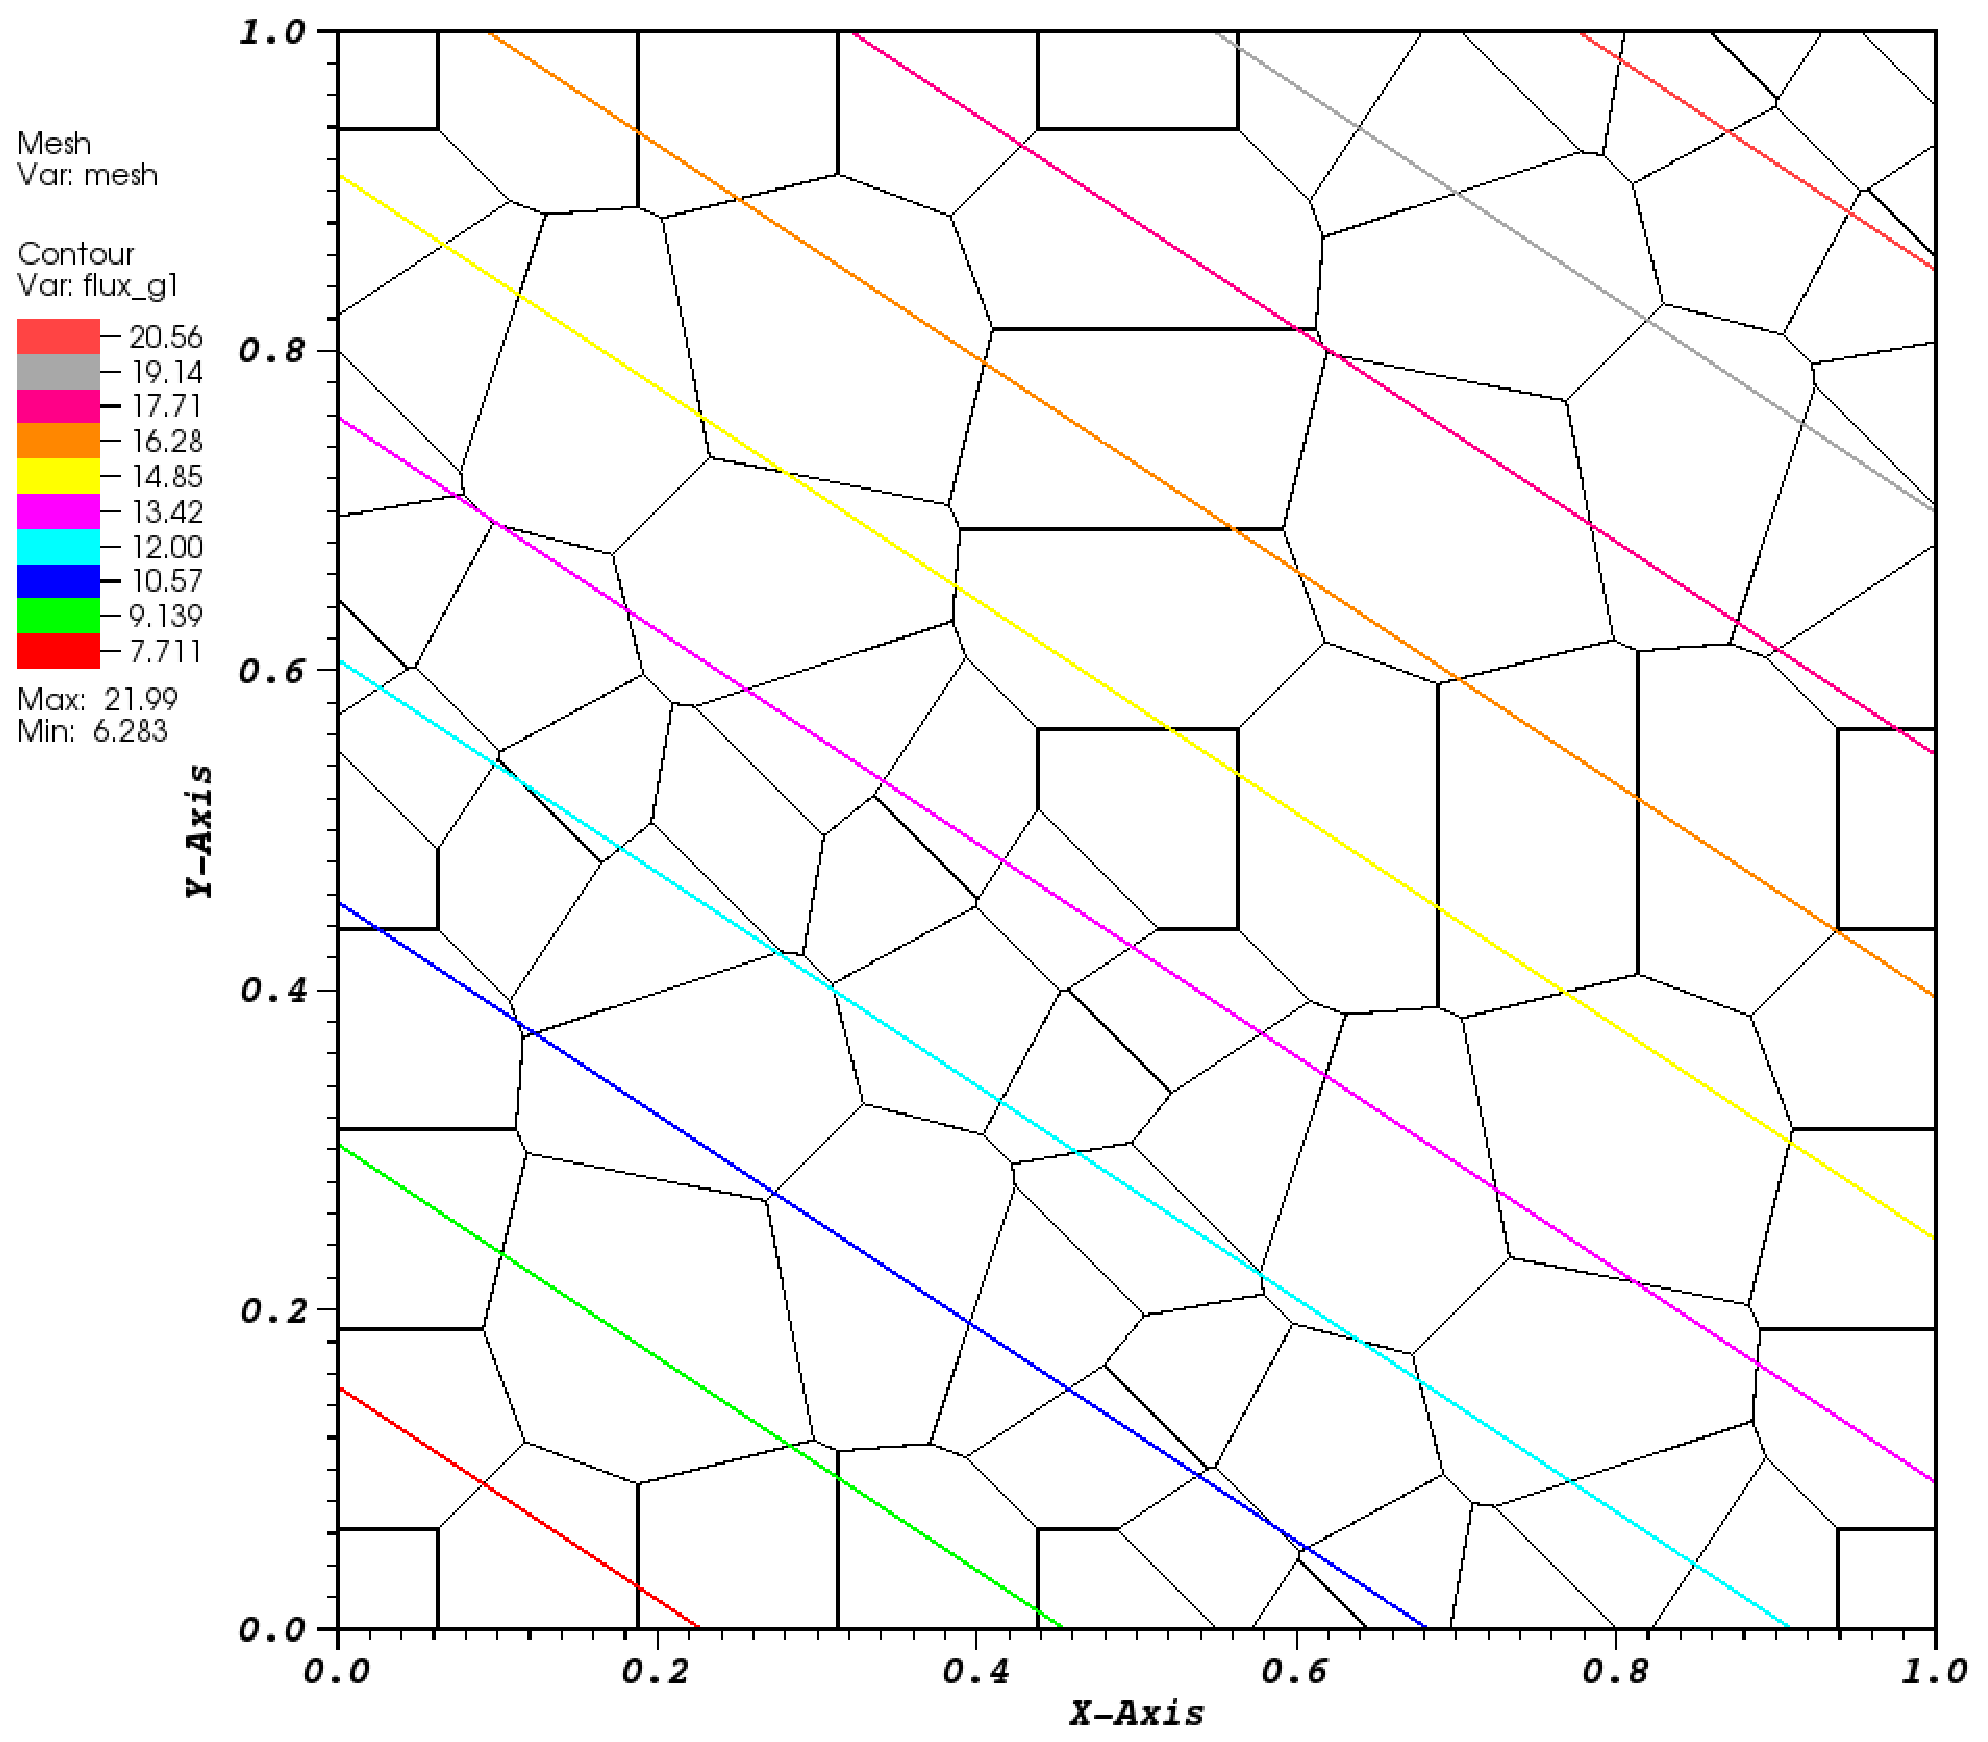
\includegraphics[width=\textwidth]{figures/sec_BF/smooth_poly_WACHSPRESS_k1.eps}
		\caption{}
	\end{subfigure}
	\vfill
	\begin{subfigure}[b]{0.45\textwidth}
		\centering
		\label{subfig::z_quad_wach_lin_sol}
		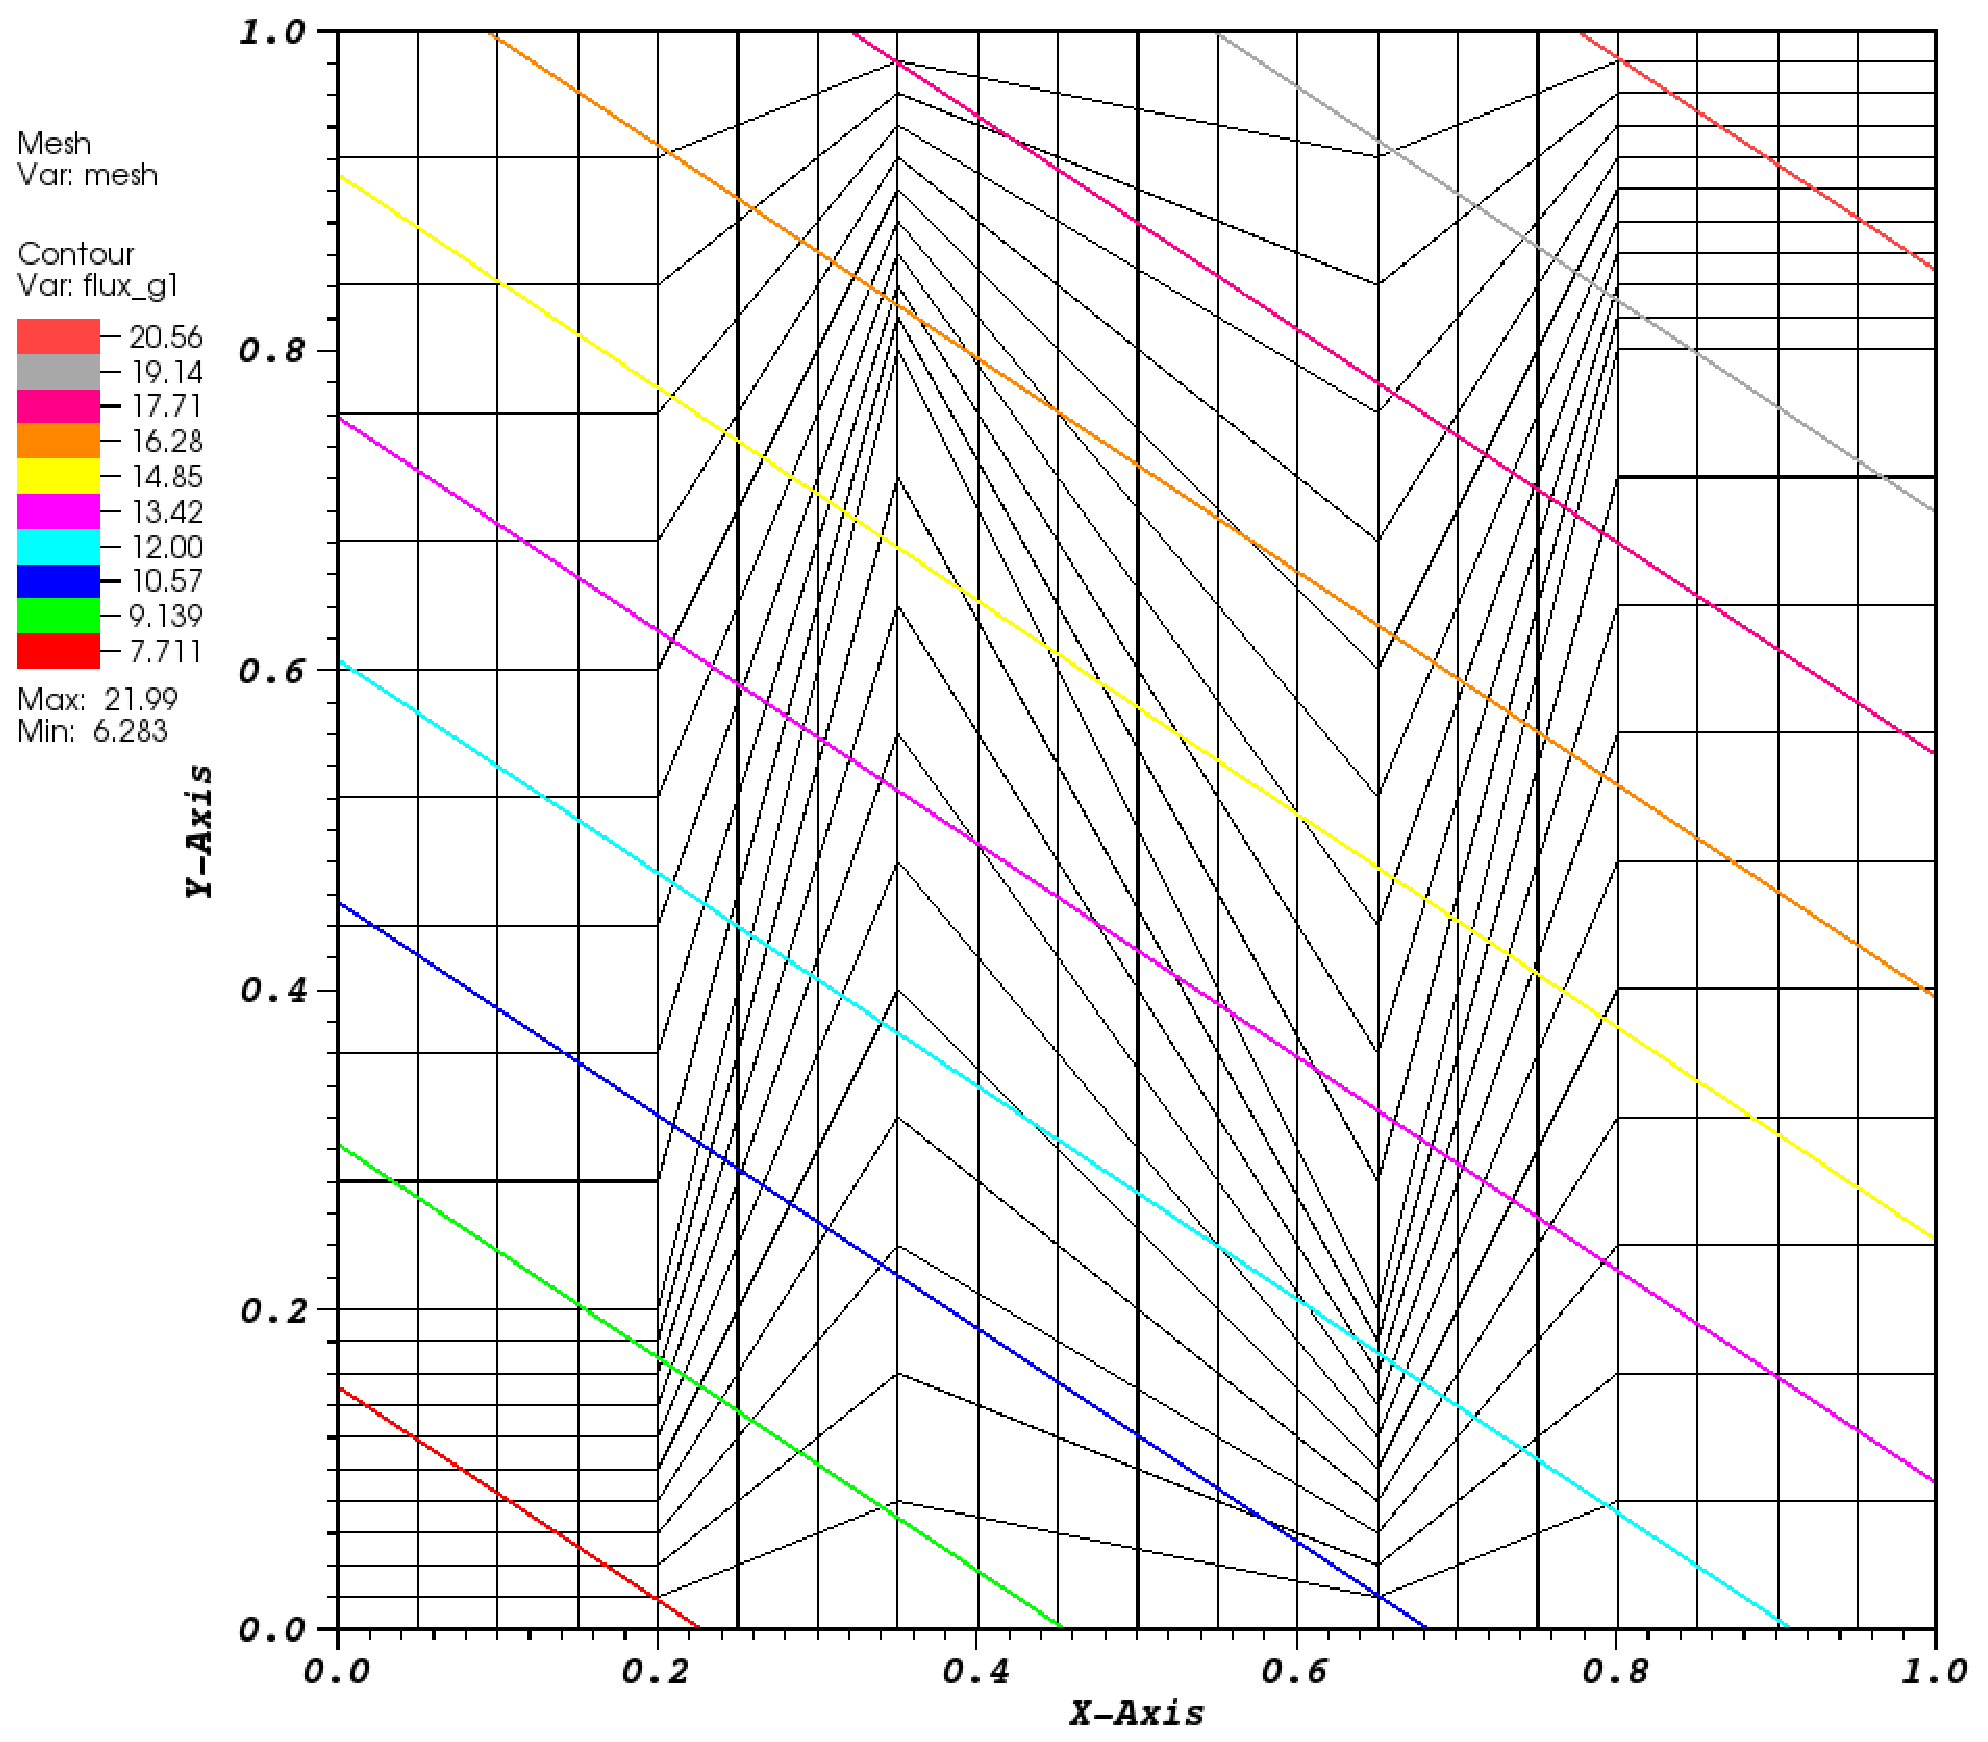
\includegraphics[width=\textwidth]{figures/sec_BF/z_quad_WACHSPRESS_k1.eps}
		\caption{}
	\end{subfigure}
	\hfill
	\begin{subfigure}[b]{0.45\textwidth}
		\centering
		\label{subfig::z_poly_wach_lin_sol}
		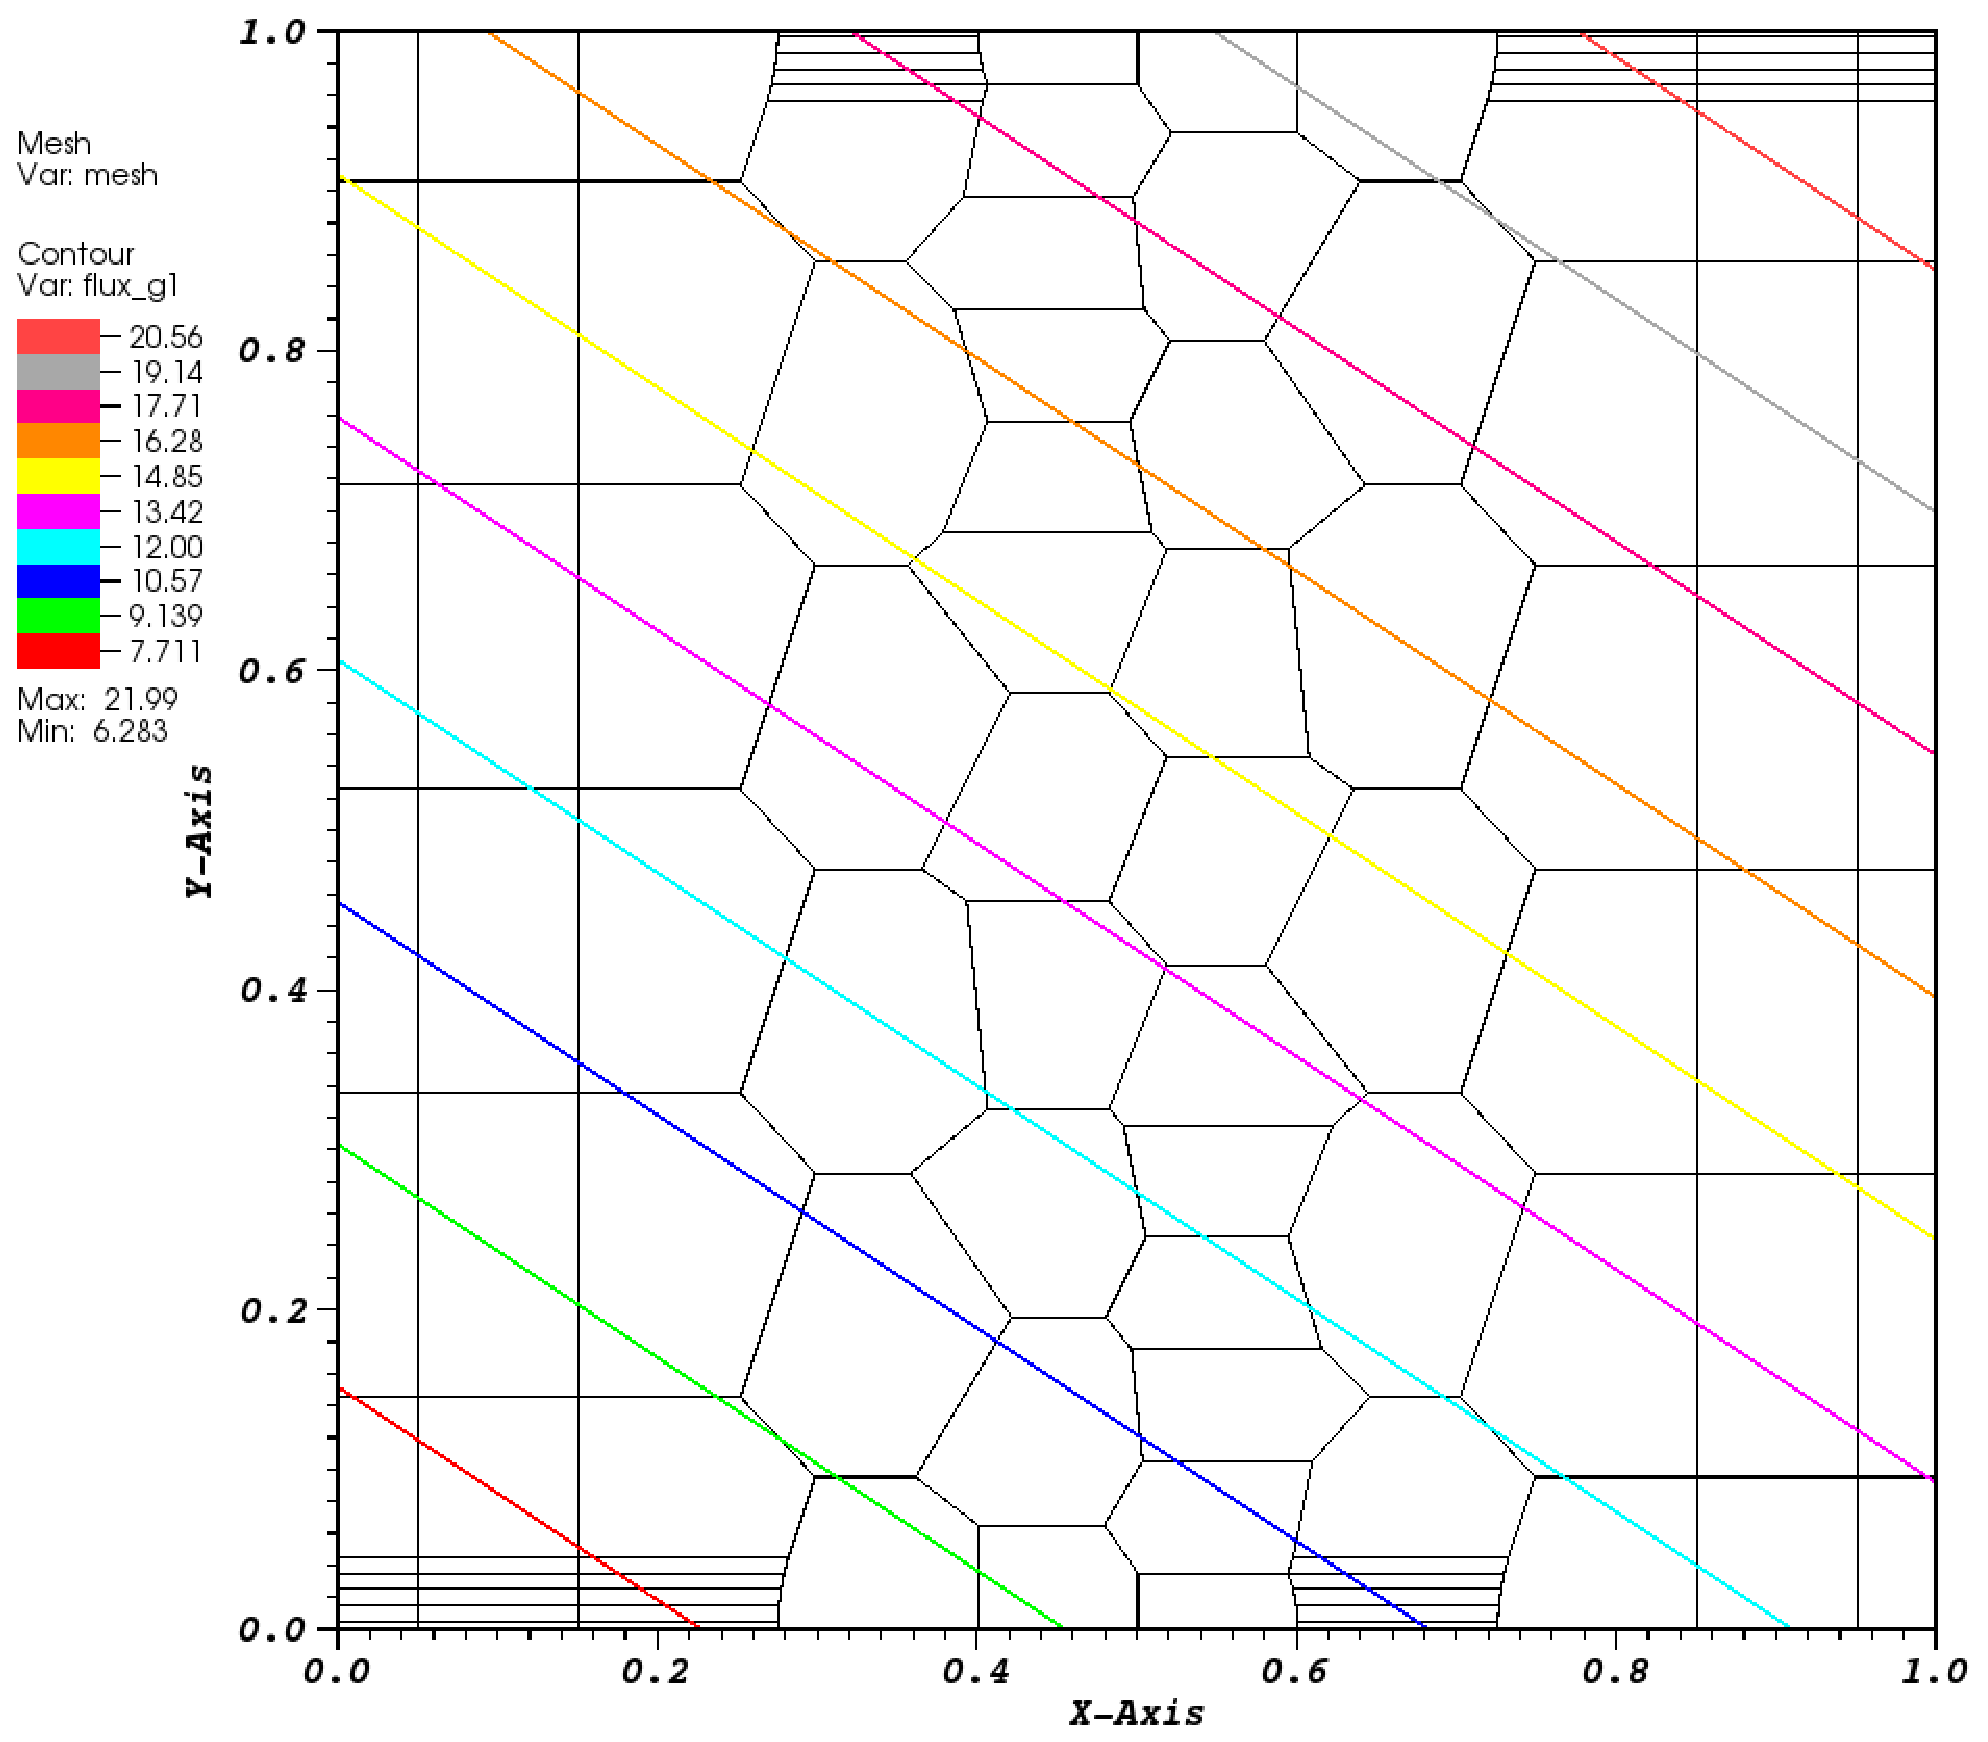
\includegraphics[width=\textwidth]{figures/sec_BF/z_poly_WACHSPRESS_k1.eps}
		\caption{}
	\end{subfigure}
\caption{Contour plots of the exactly-linear solution with the Wachspress basis functions on (a) cartesian mesh, (b) ordered-triangular mesh, (c) quadrilateral shestakov mesh, (d) sinusoidal polygonal mesh, (e) quadrilateral z-mesh, and (f) polygonal z-mesh.}
\label{fig::BF_Results_Linear_wach_sol}
\end{figure}

\begin{figure}
\centering
	\begin{subfigure}[b]{0.45\textwidth}
		\centering
		\label{subfig::cart_pwld_lin_sol}
		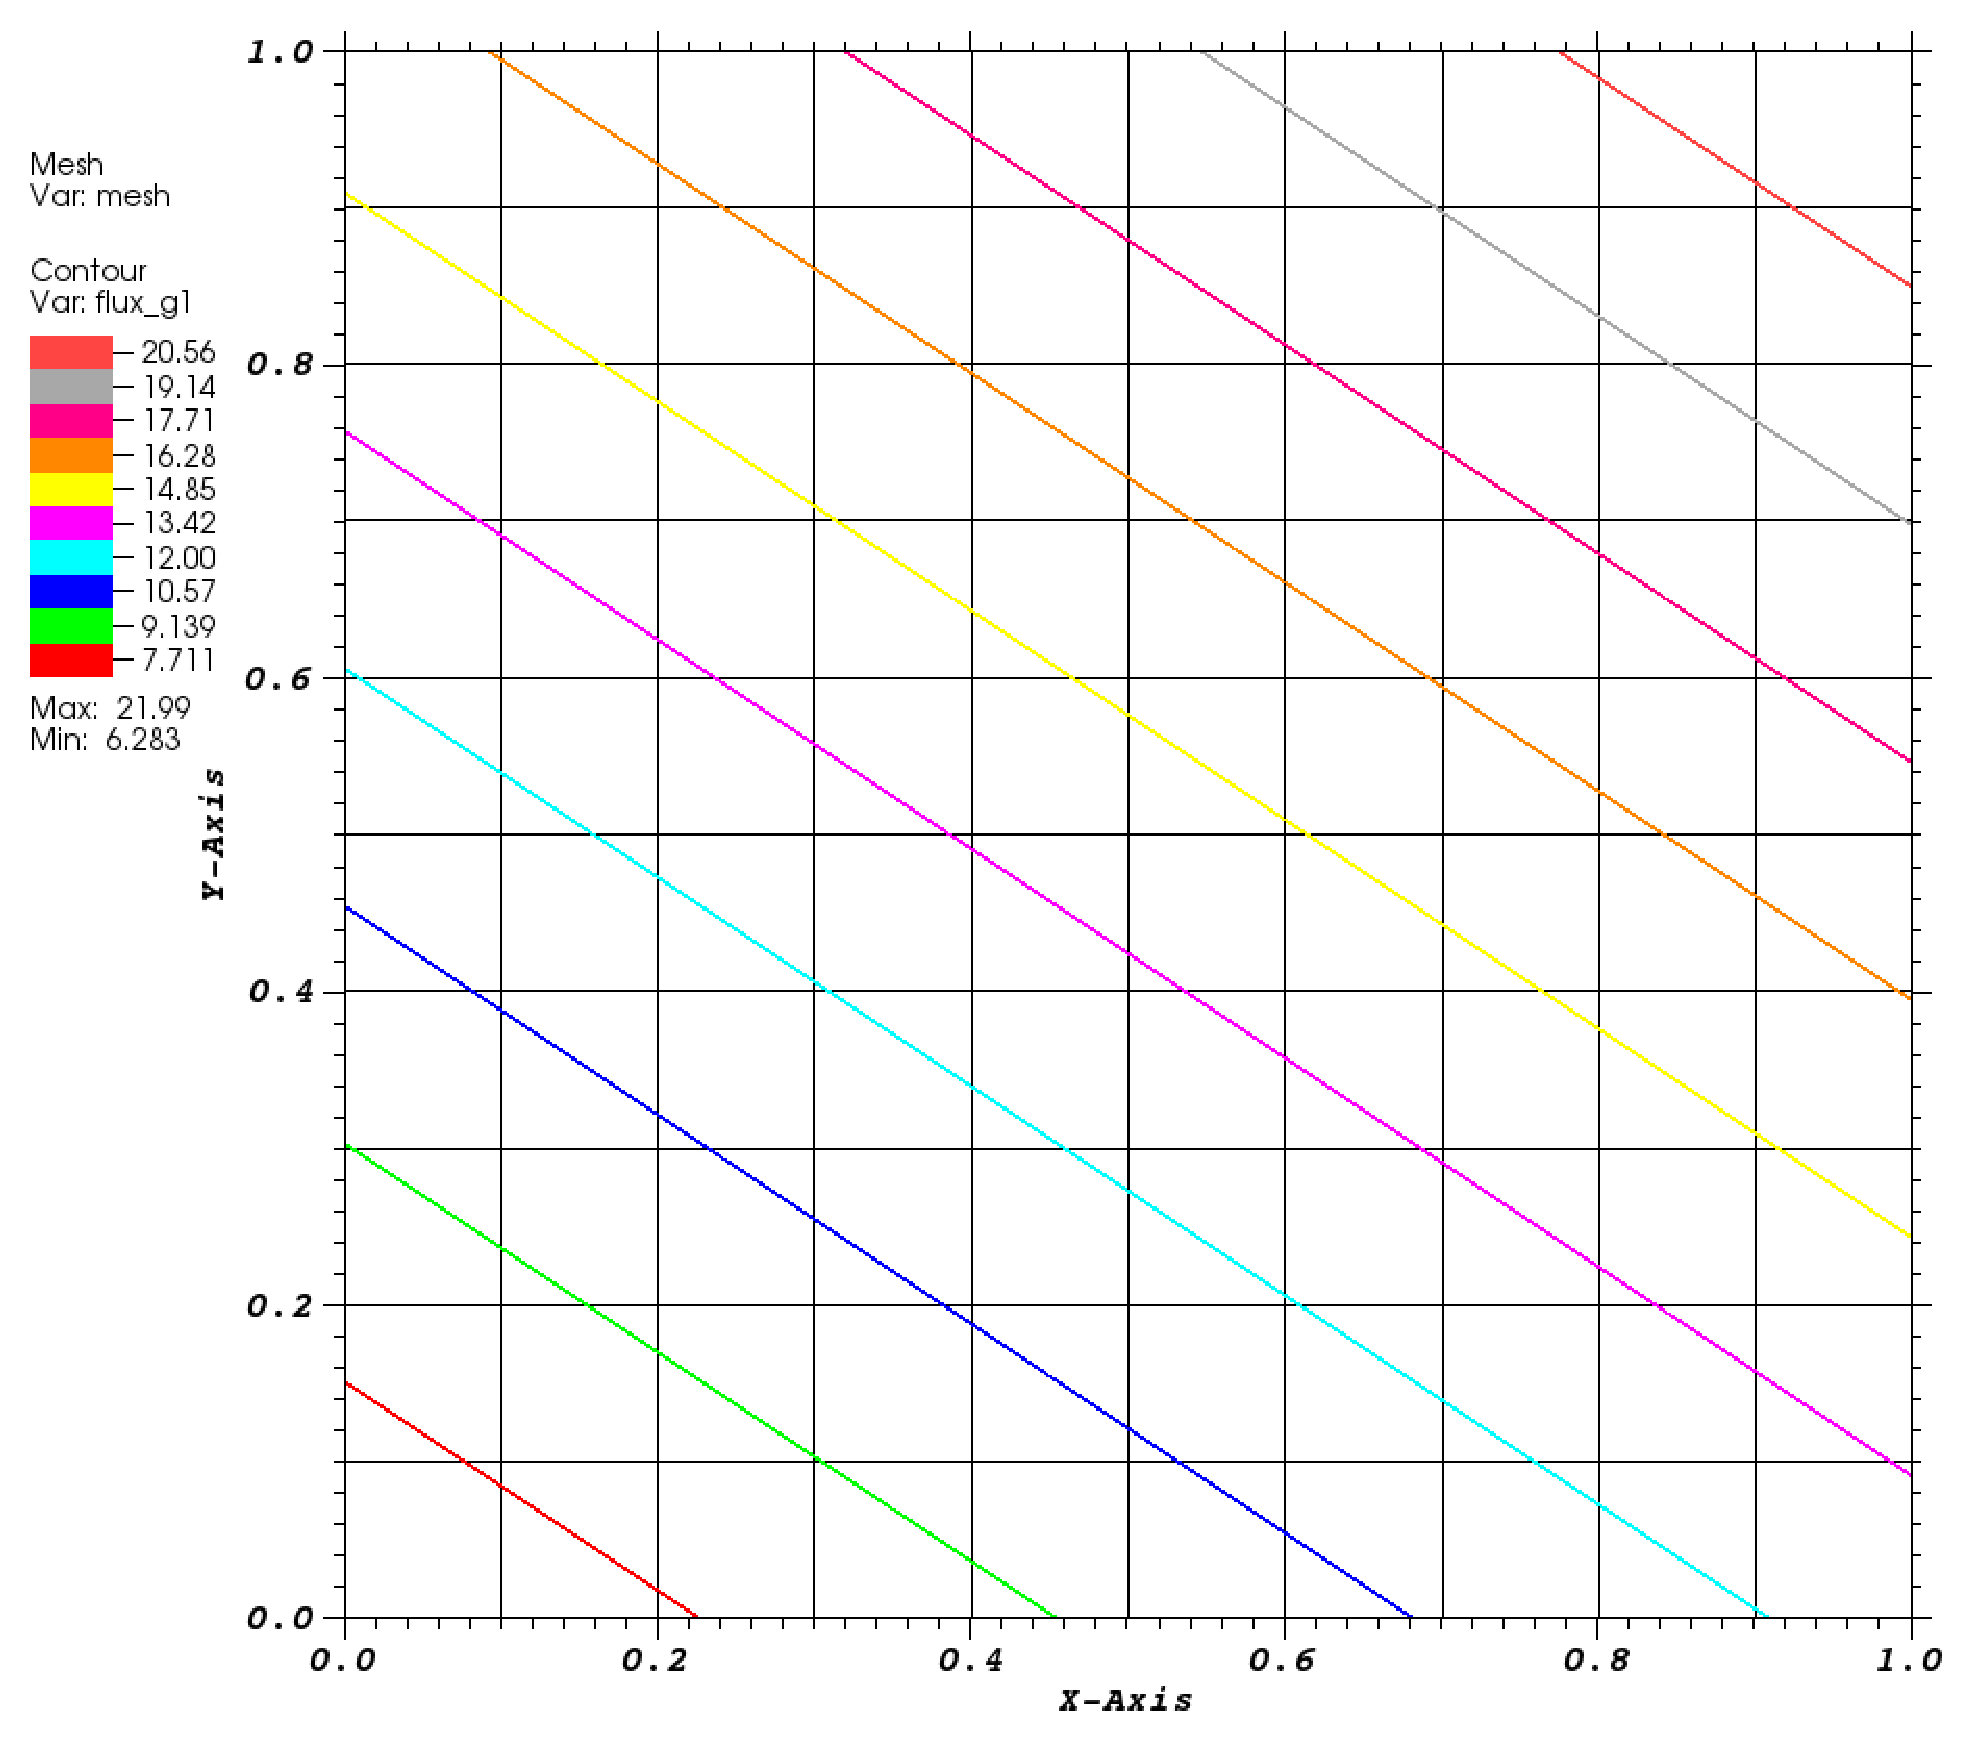
\includegraphics[width=\textwidth]{figures/sec_BF/cart_PWLD_k1.eps}
		\caption{}
	\end{subfigure}
	\hfill
	\begin{subfigure}[b]{0.45\textwidth}
		\centering
		\label{subfig::tri_pwld_lin_sol}
		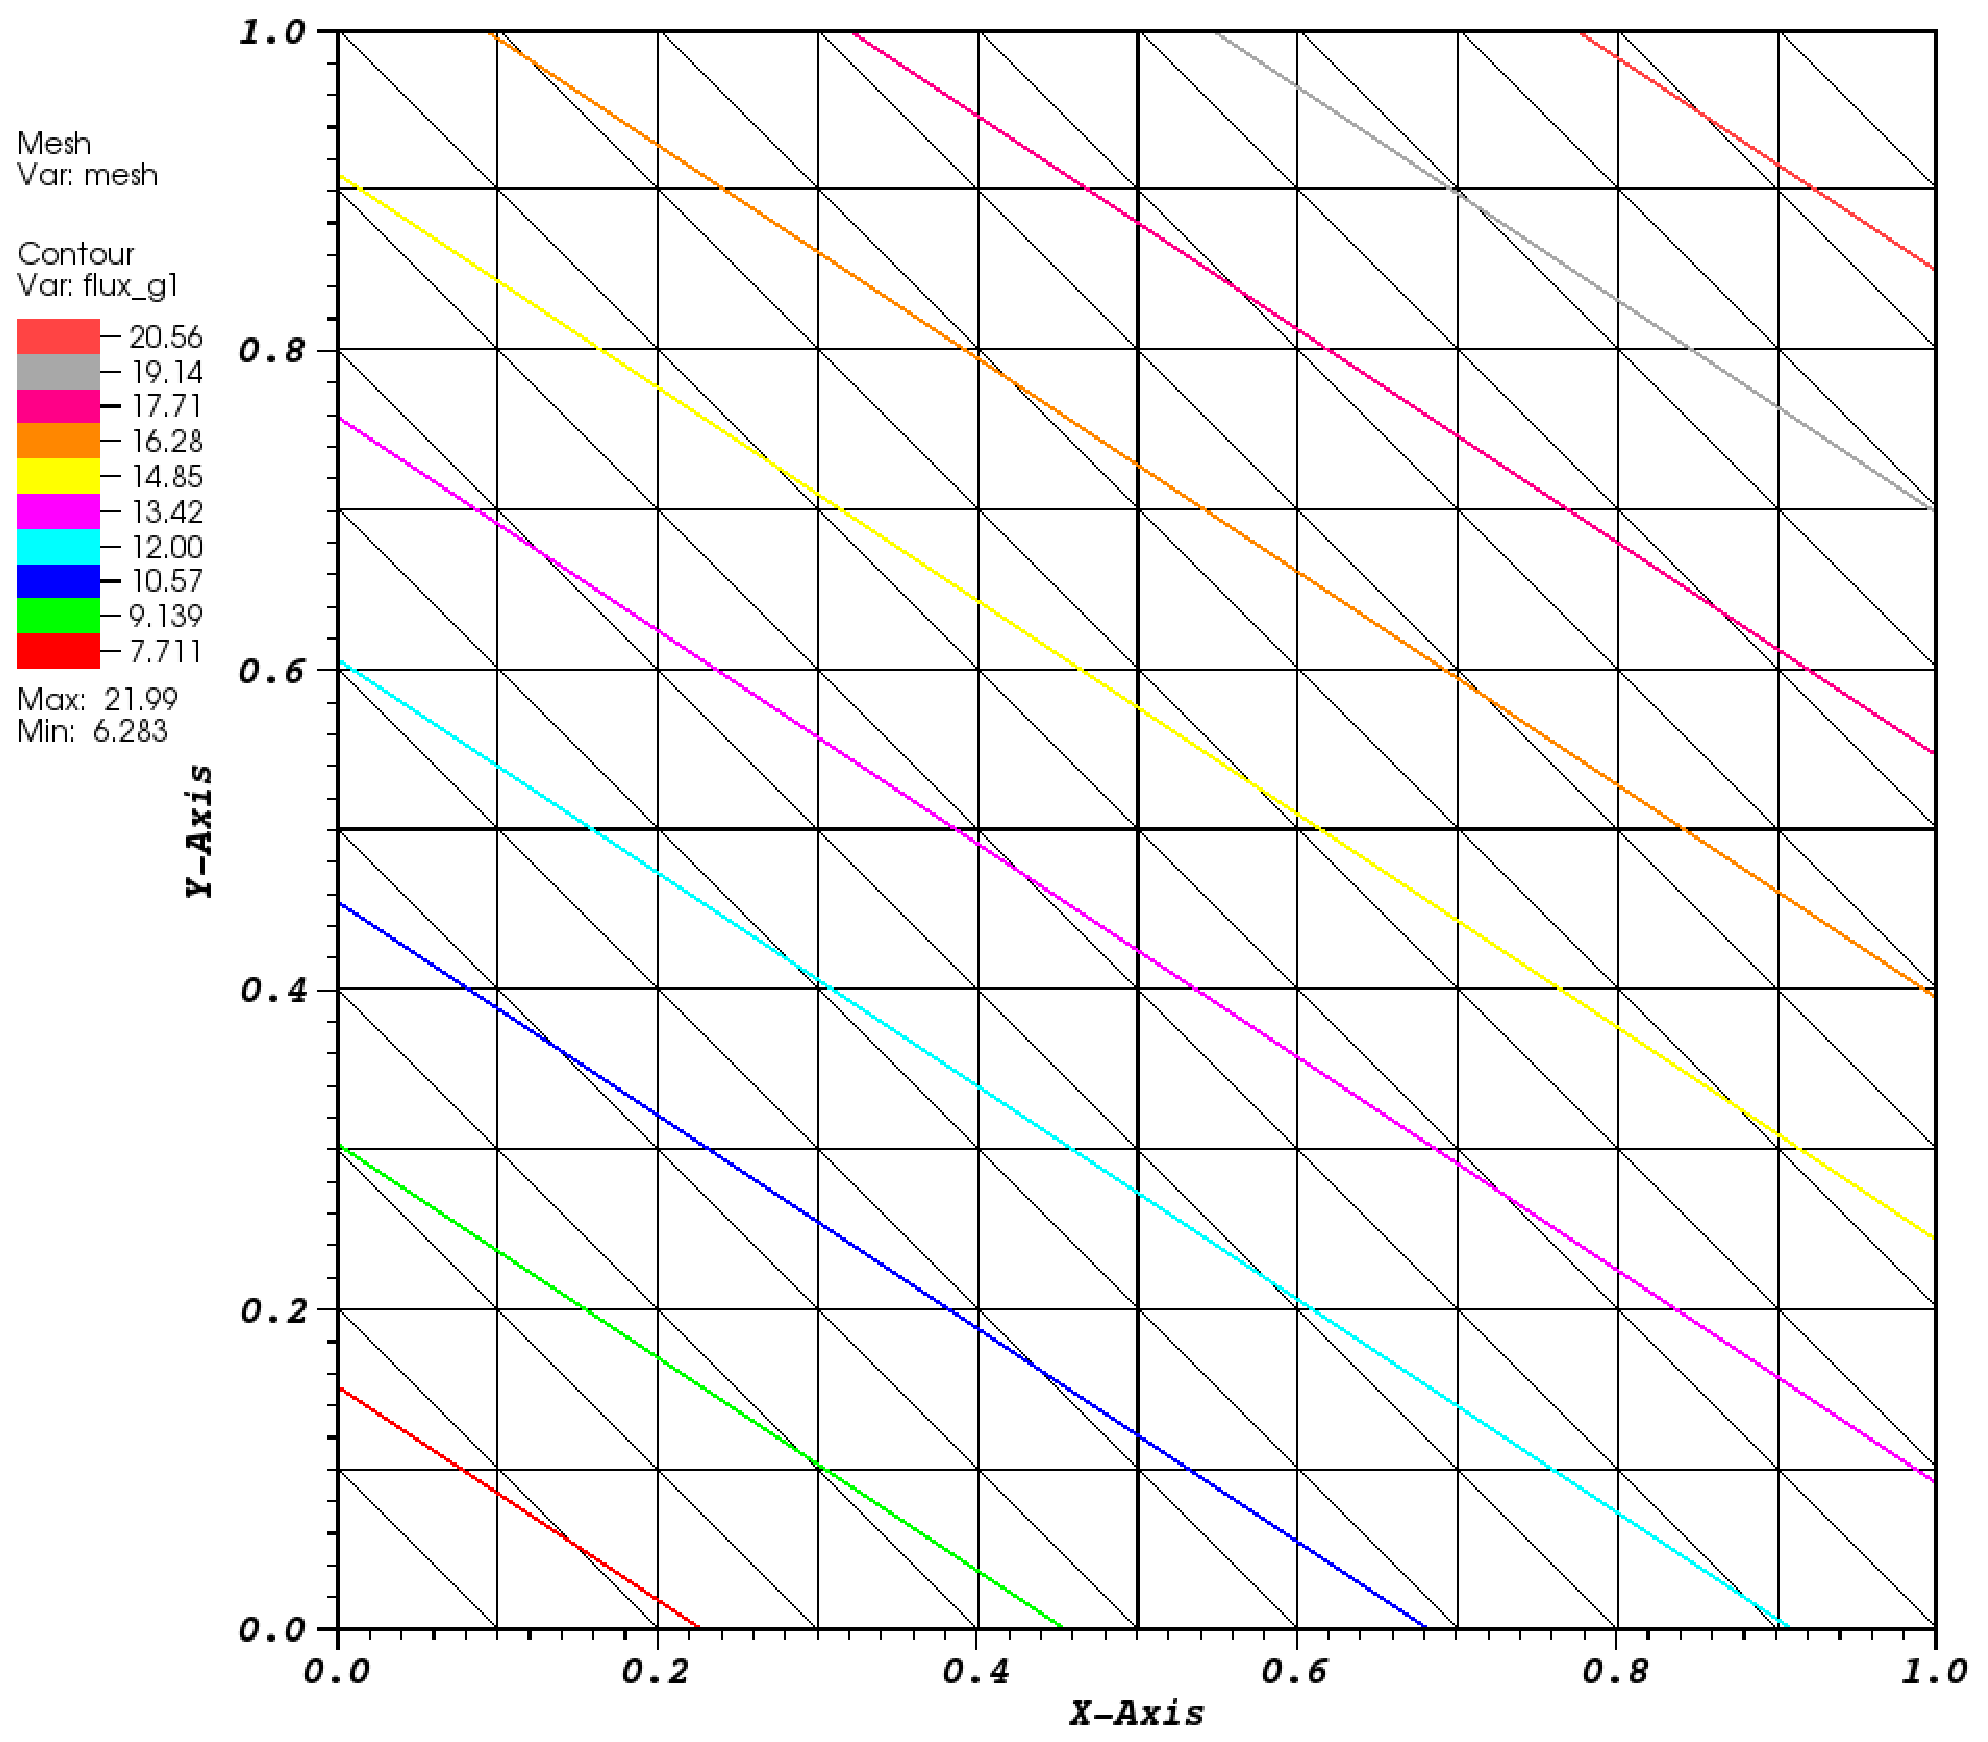
\includegraphics[width=\textwidth]{figures/sec_BF/tri_PWLD_k1.eps}
		\caption{}
	\end{subfigure}
	\vfill
	\begin{subfigure}[b]{0.45\textwidth}
		\centering
		\label{subfig::shes_quad_pwld_lin_sol}
		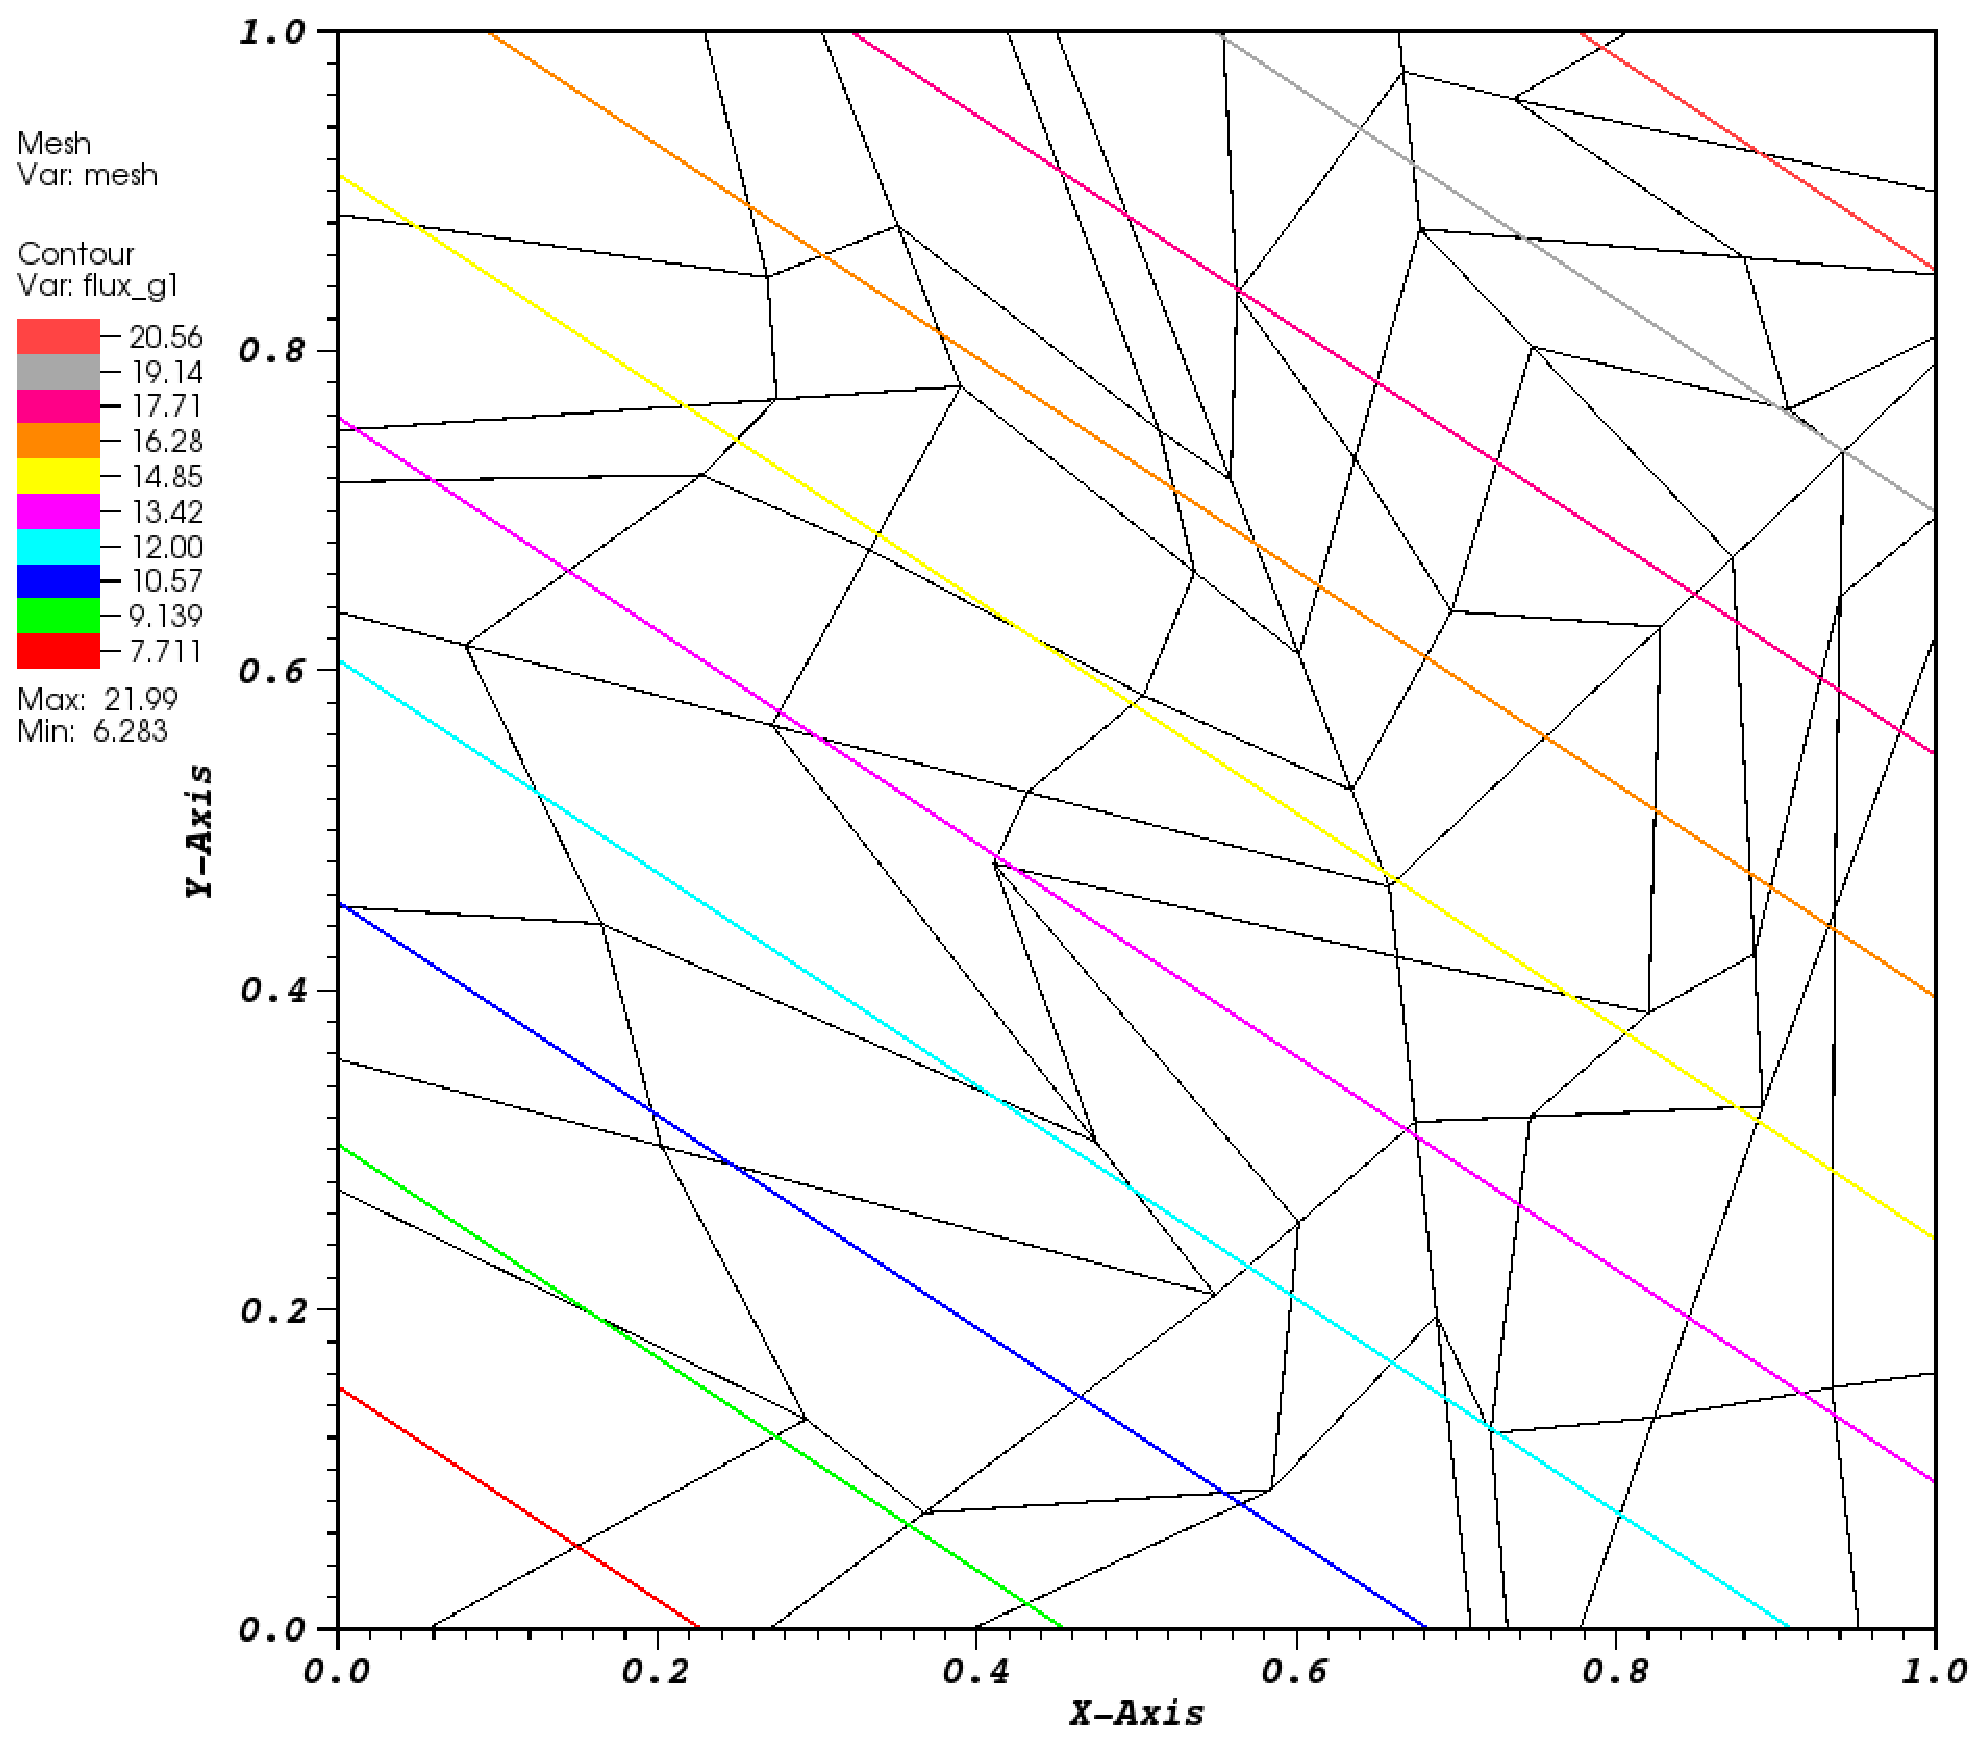
\includegraphics[width=\textwidth]{figures/sec_BF/shes_quad_PWLD_k1.eps}
		\caption{}
	\end{subfigure}
	\hfill
	\begin{subfigure}[b]{0.45\textwidth}
		\centering
		\label{subfig::smooth_poly_pwld_lin_sol}
		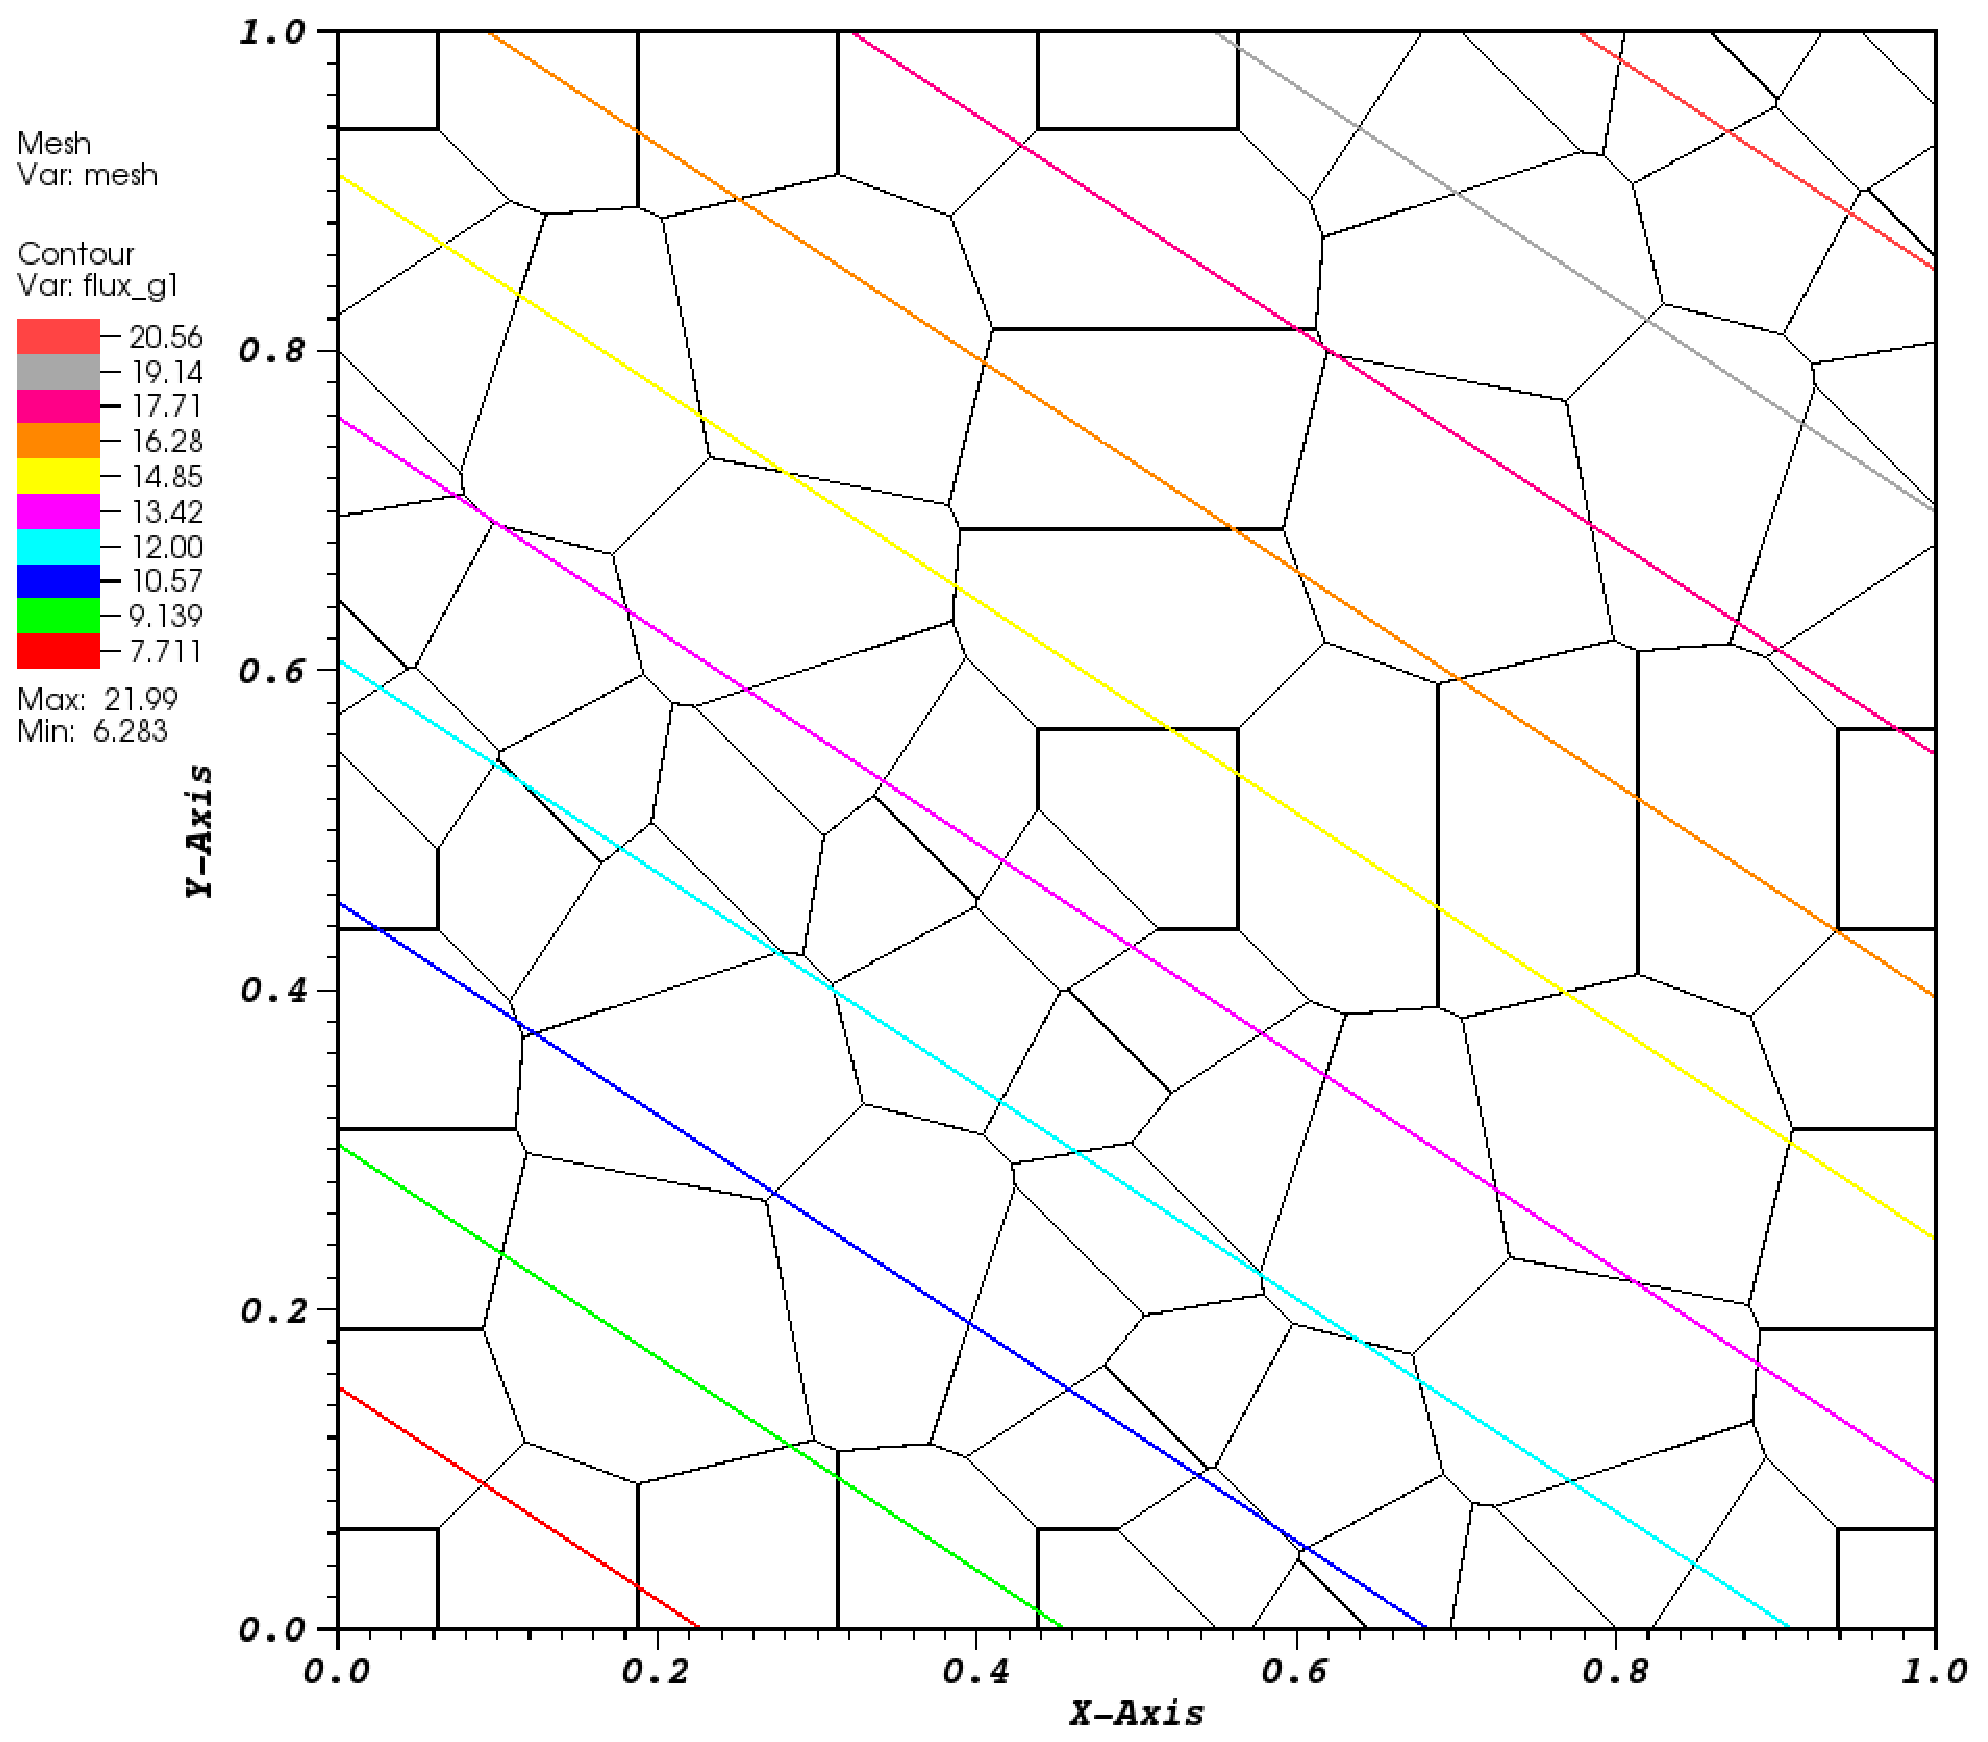
\includegraphics[width=\textwidth]{figures/sec_BF/smooth_poly_PWLD_k1.eps}
		\caption{}
	\end{subfigure}
	\vfill
	\begin{subfigure}[b]{0.45\textwidth}
		\centering
		\label{subfig::z_quad_pwld_lin_sol}
		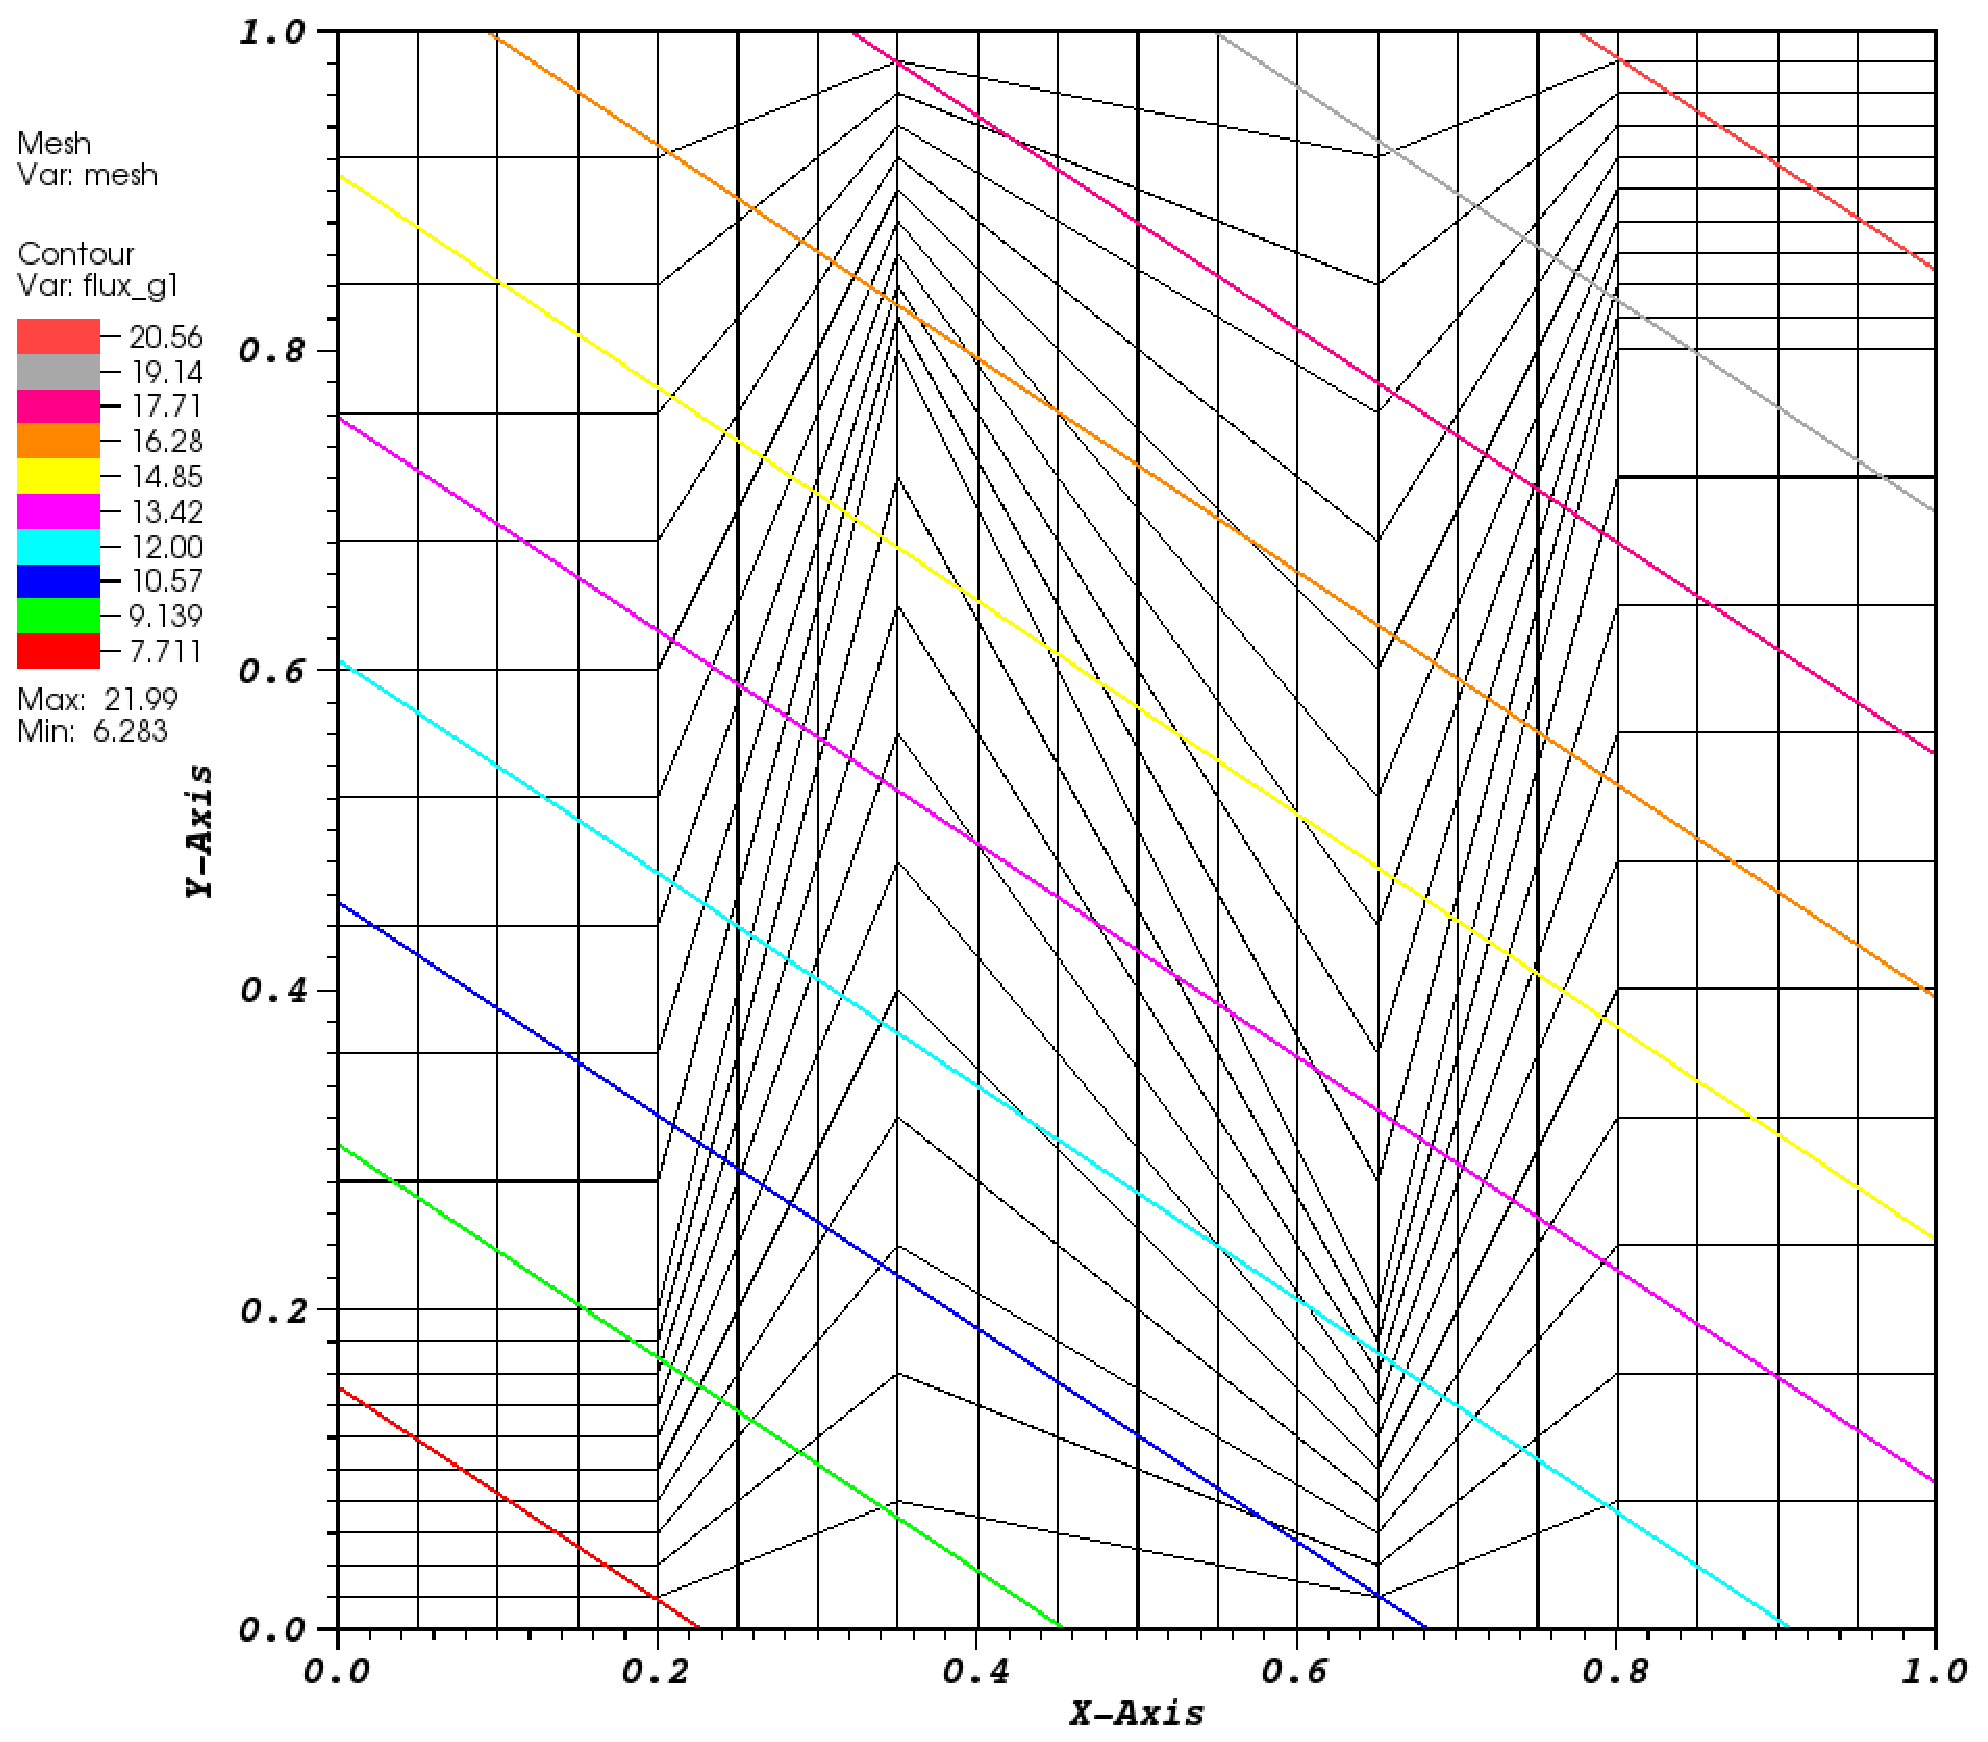
\includegraphics[width=\textwidth]{figures/sec_BF/z_quad_PWLD_k1.eps}
		\caption{}
	\end{subfigure}
	\hfill
	\begin{subfigure}[b]{0.45\textwidth}
		\centering
		\label{subfig::z_poly_pwld_lin_sol}
		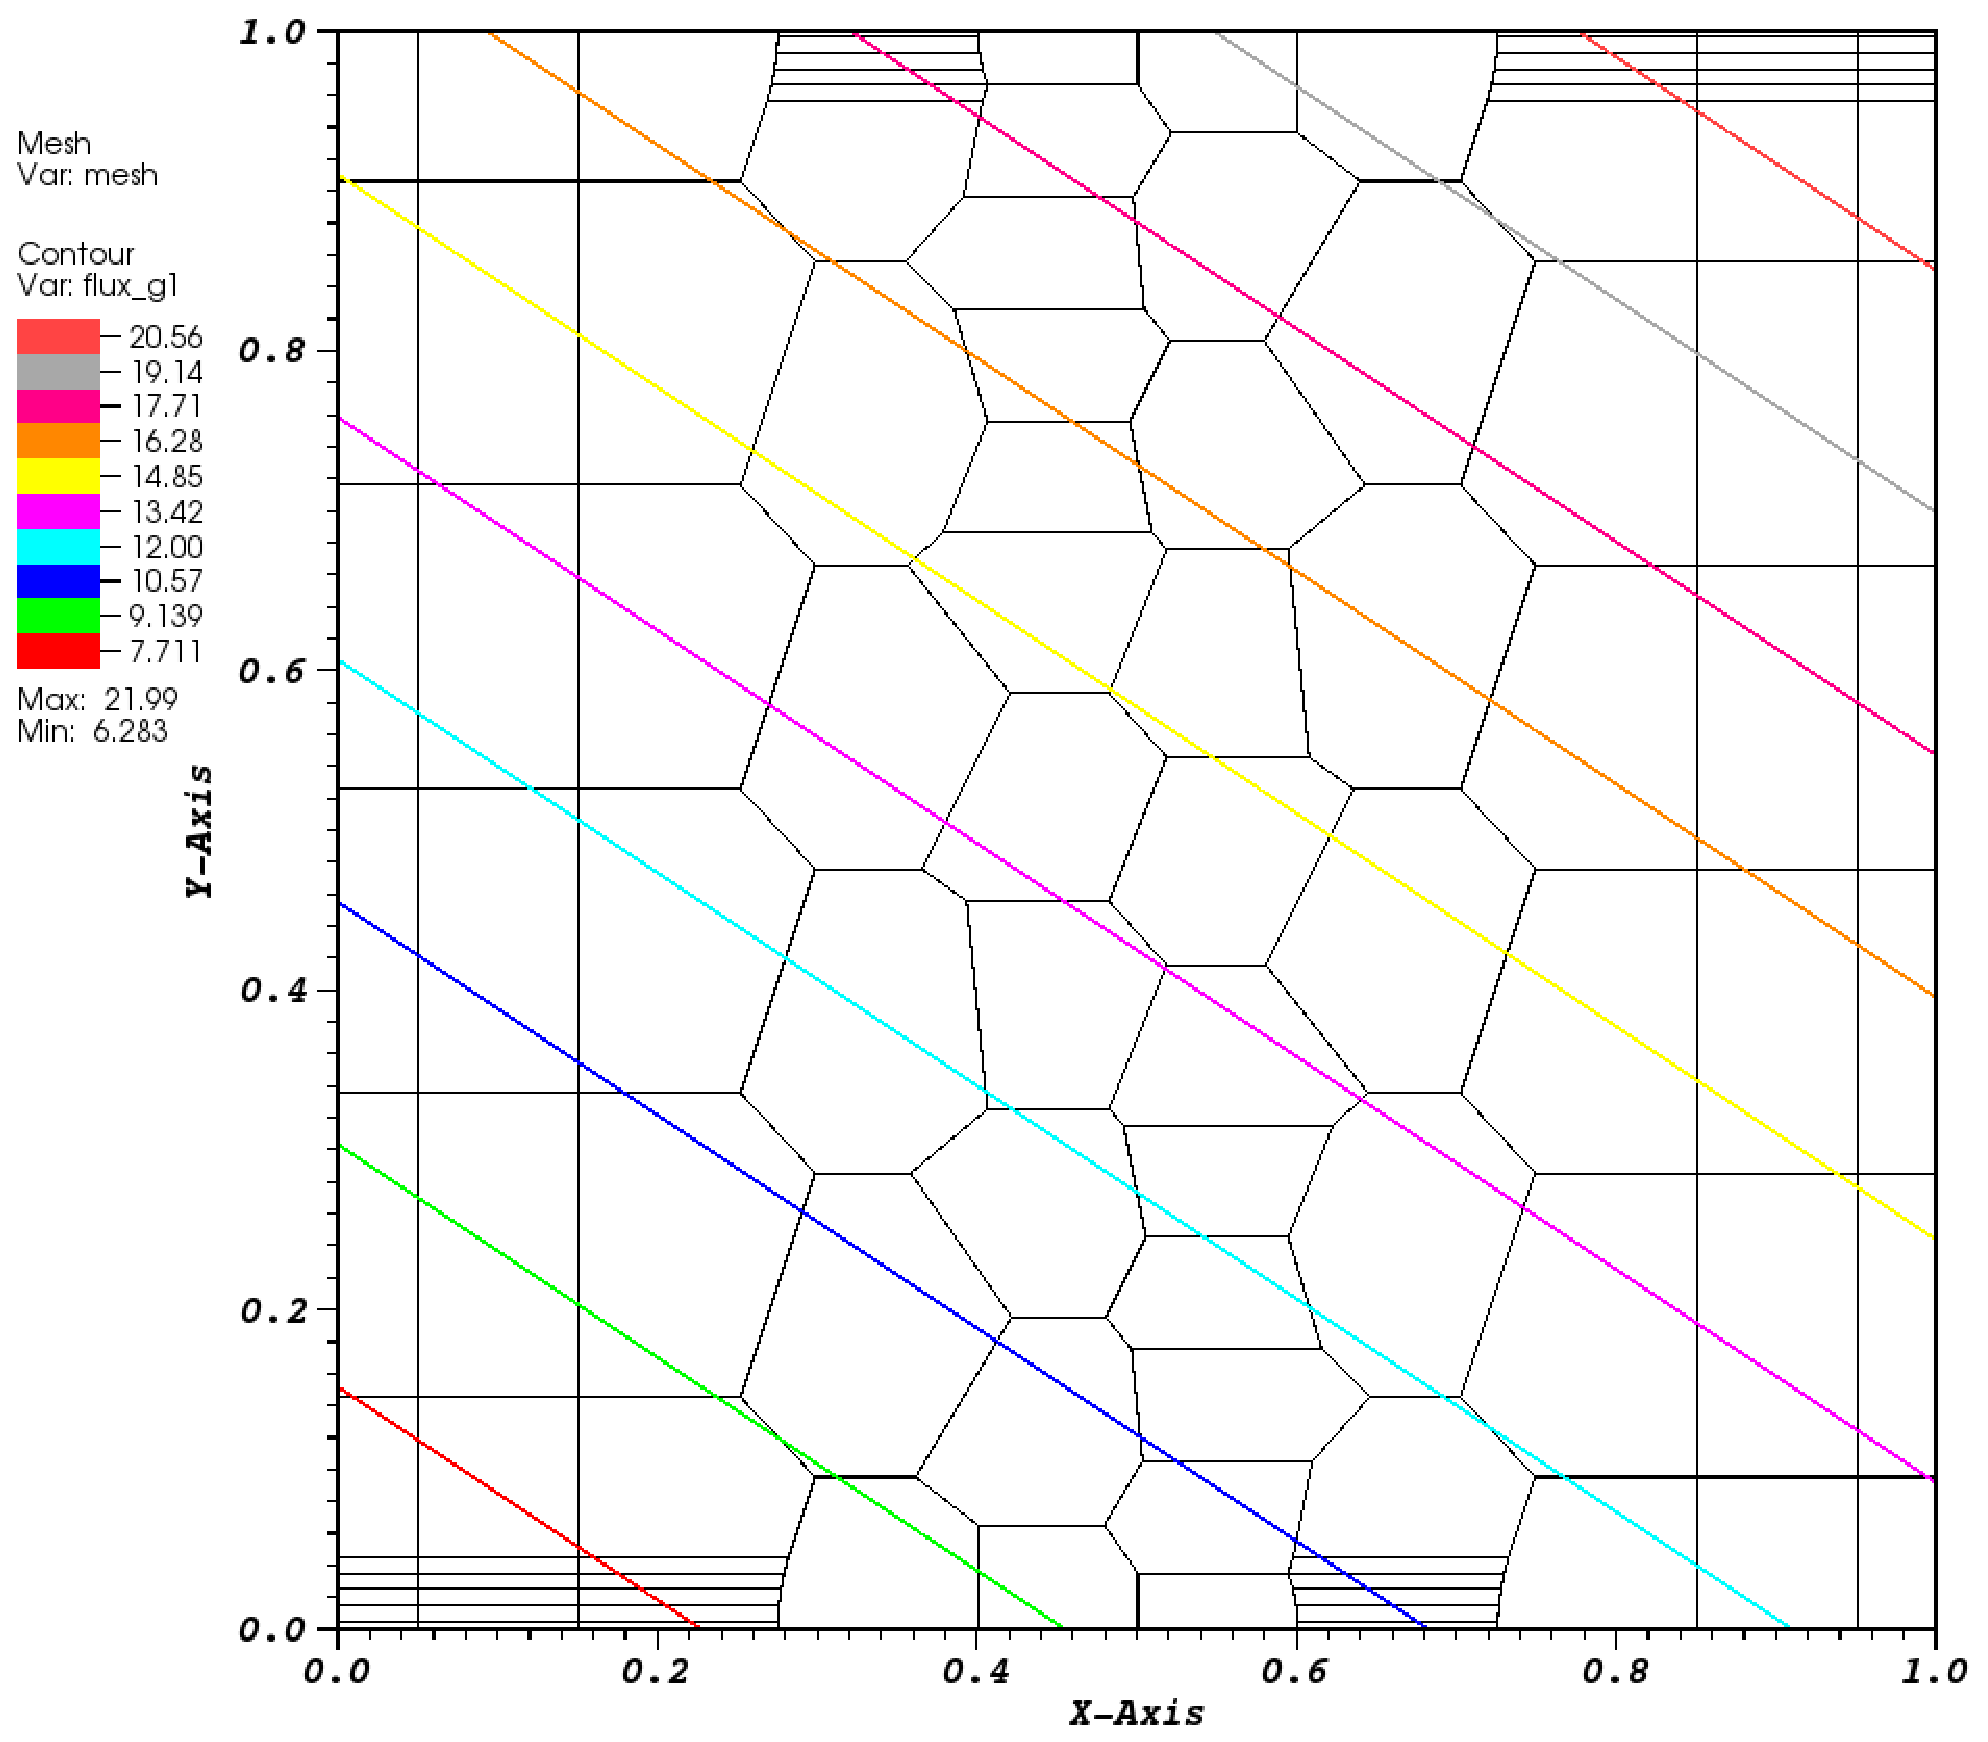
\includegraphics[width=\textwidth]{figures/sec_BF/z_poly_PWLD_k1.eps}
		\caption{}
	\end{subfigure}
\caption{Contour plots of the exactly-linear solution with the PWL basis functions on (a) cartesian mesh, (b) ordered-triangular mesh, (c) quadrilateral shestakov mesh, (d) sinusoidal polygonal mesh, (e) quadrilateral z-mesh, and (f) polygonal z-mesh.}
\label{fig::BF_Results_Linear_pwld_sol}
\end{figure}

\begin{figure}
\centering
	\begin{subfigure}[b]{0.45\textwidth}
		\centering
		\label{subfig::cart_mv_lin_sol}
		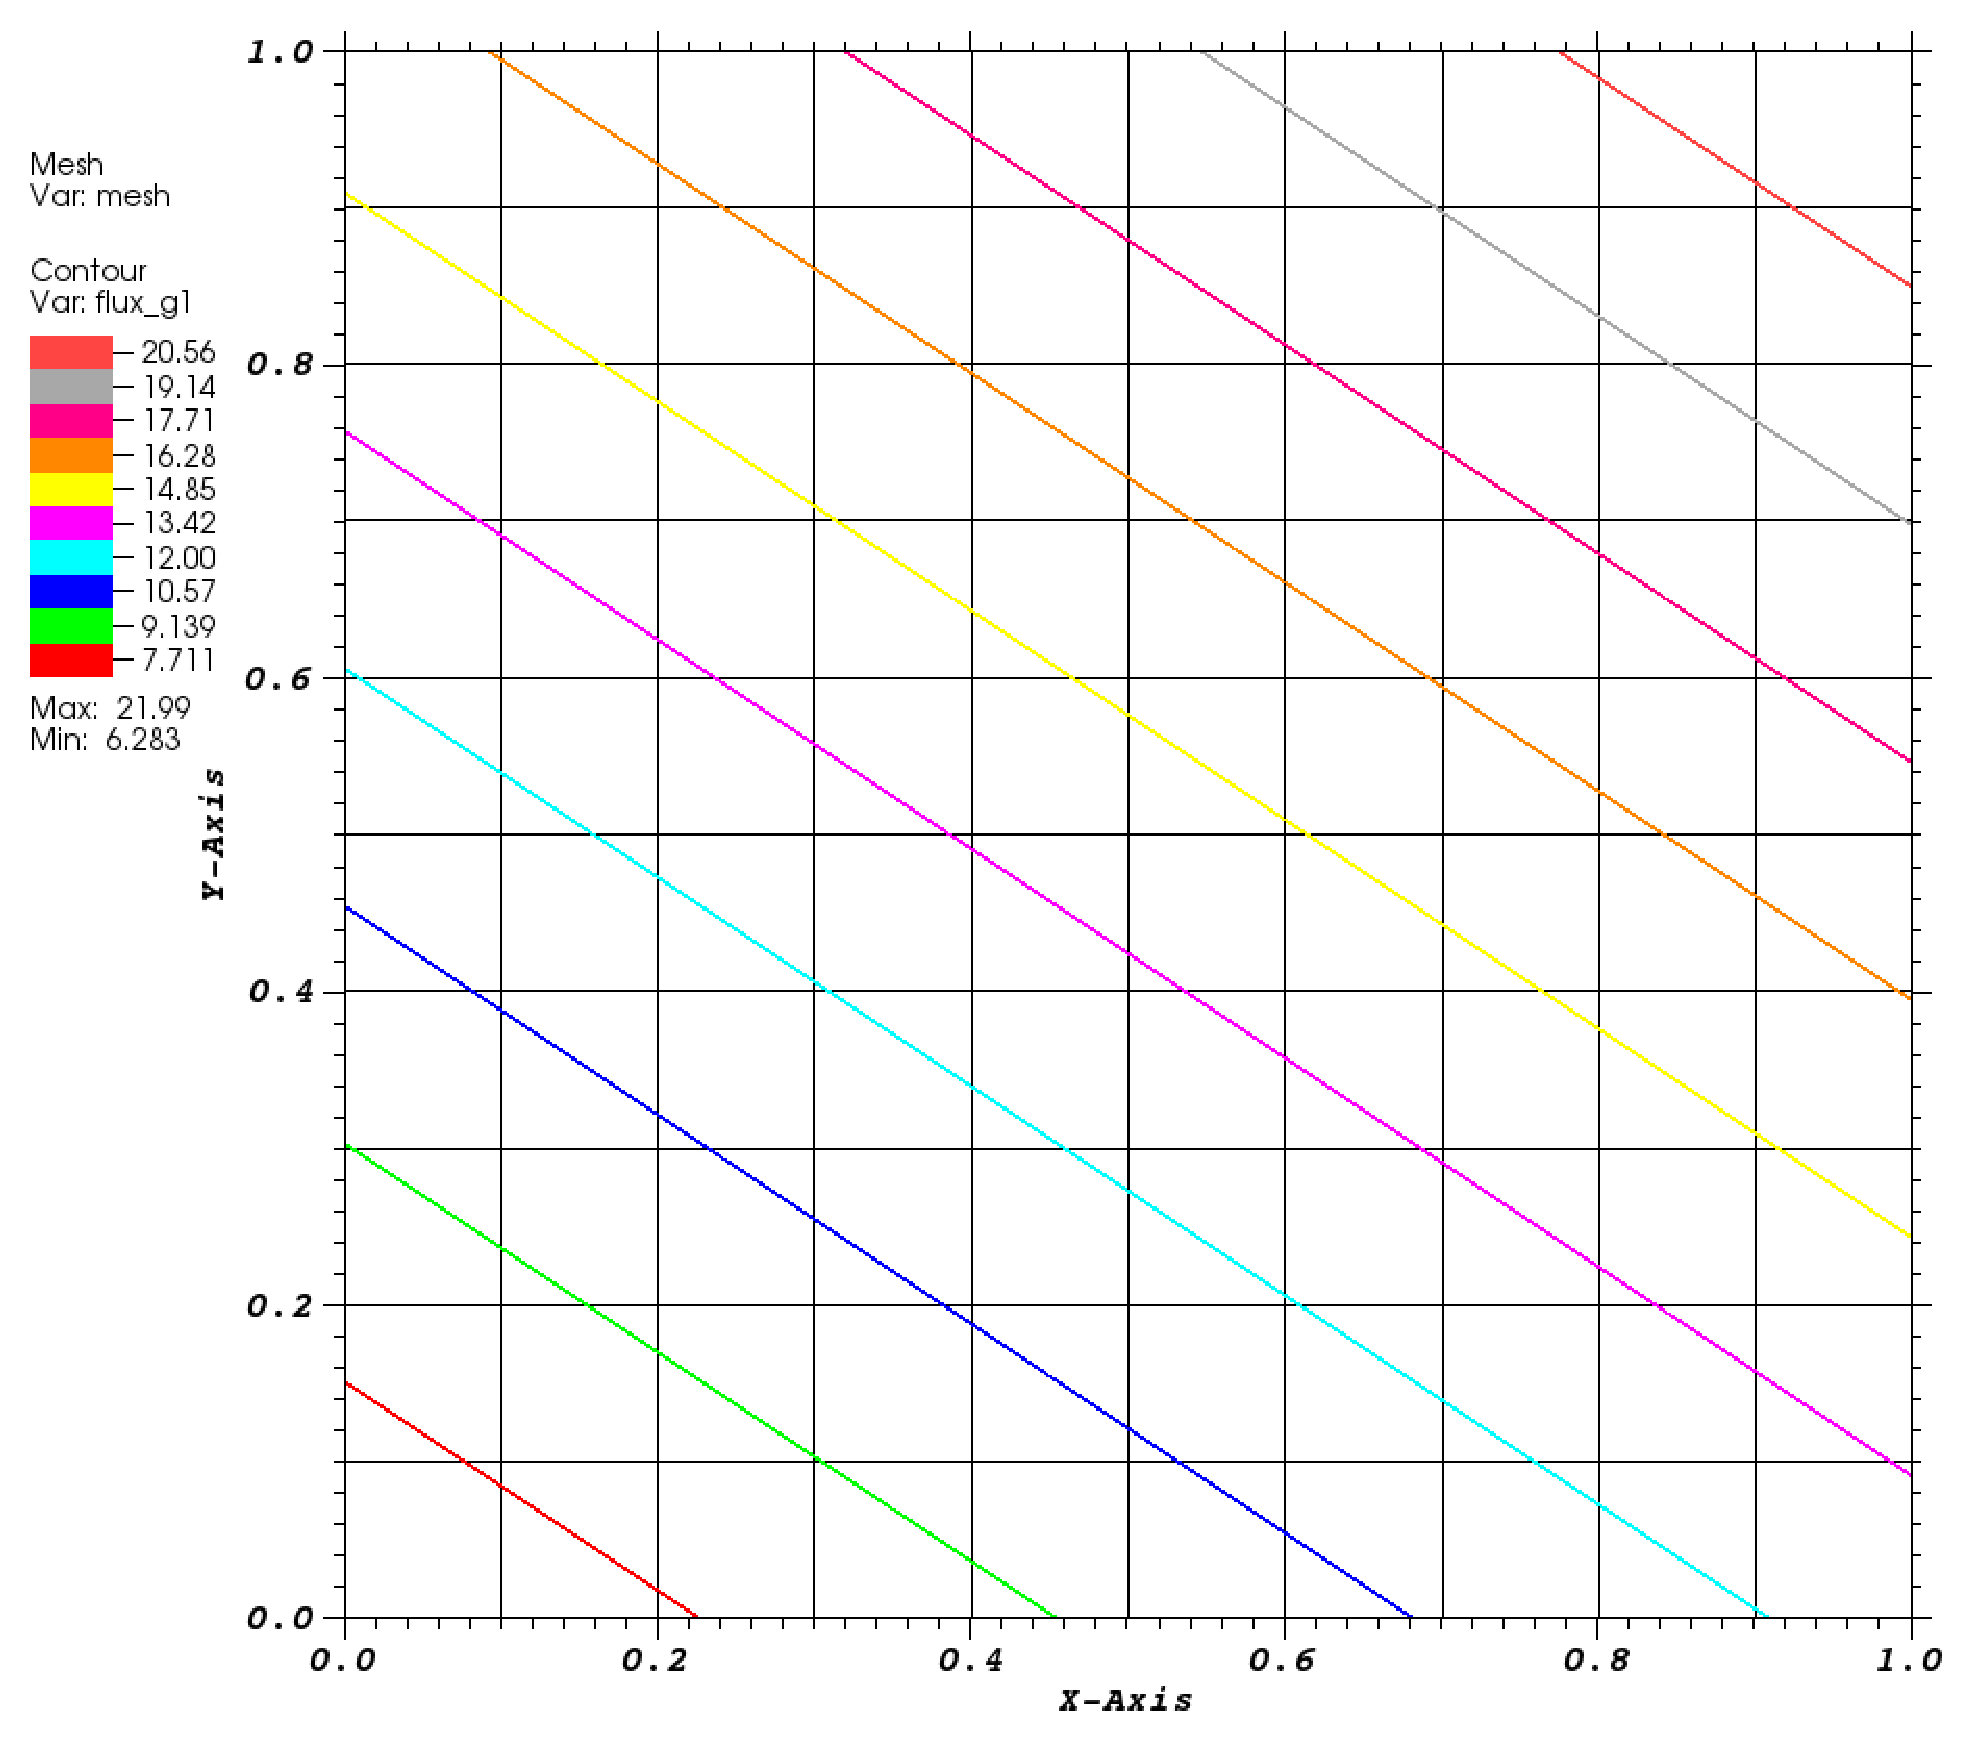
\includegraphics[width=\textwidth]{figures/sec_BF/cart_MV_k1.eps}
		\caption{}
	\end{subfigure}
	\hfill
	\begin{subfigure}[b]{0.45\textwidth}
		\centering
		\label{subfig::tri_mv_lin_sol}
		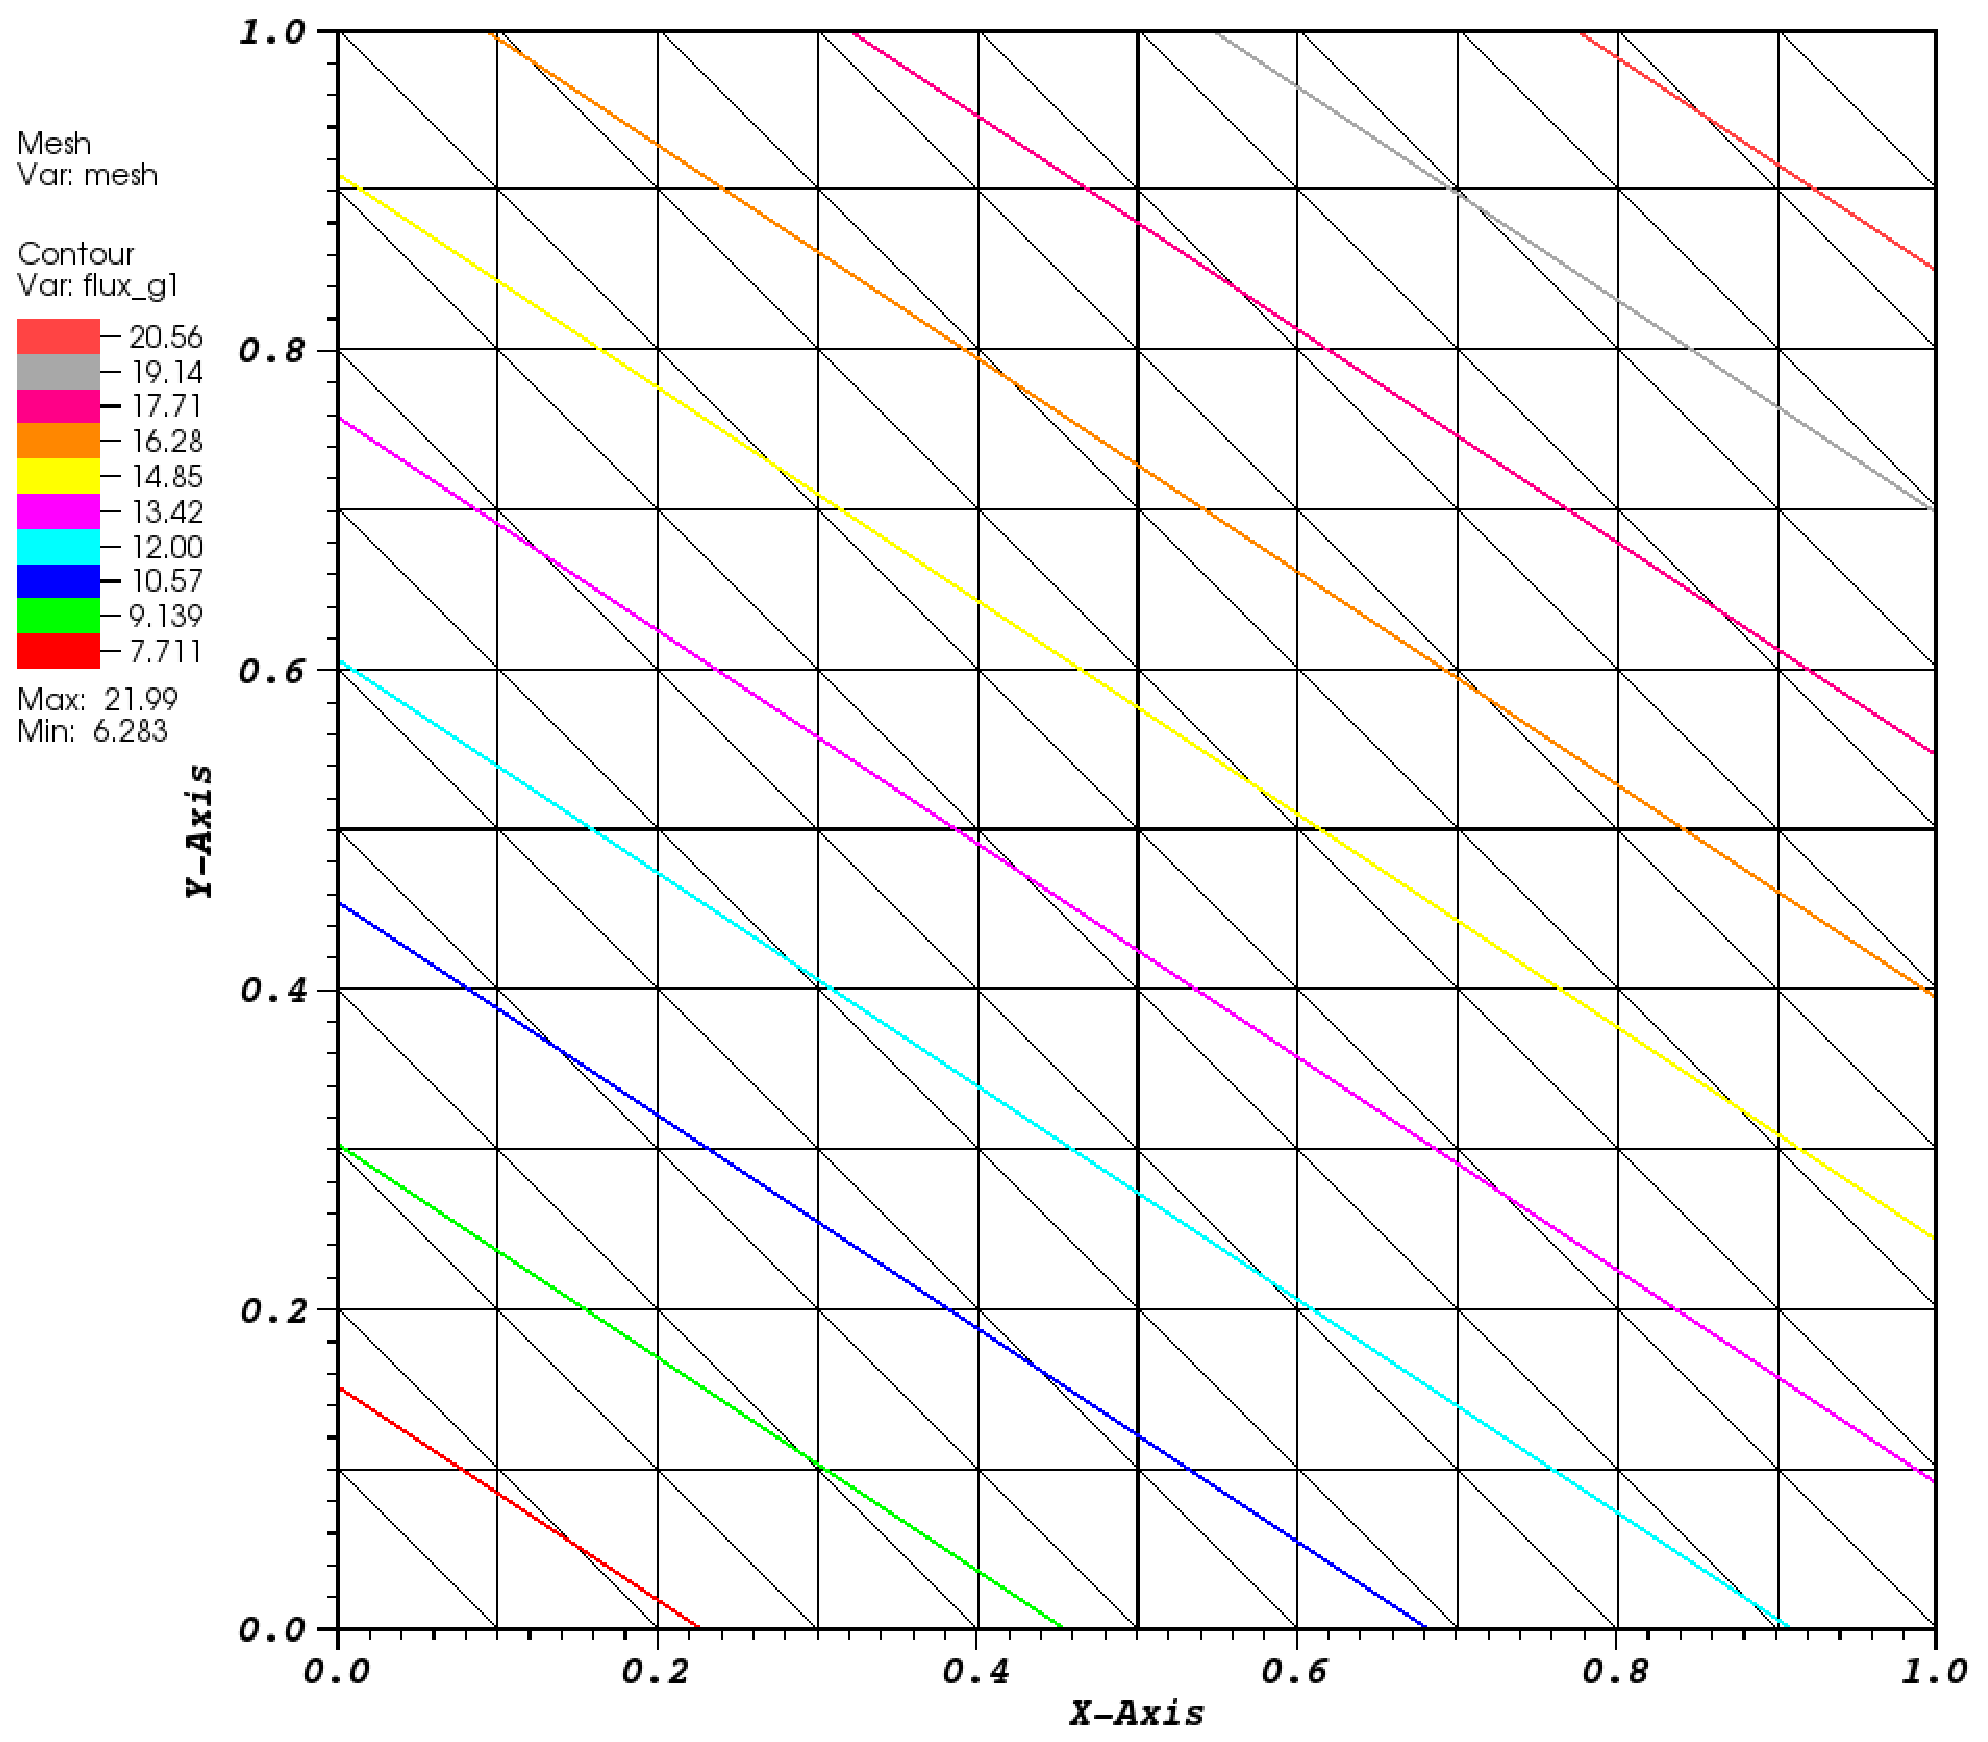
\includegraphics[width=\textwidth]{figures/sec_BF/tri_MV_k1.eps}
		\caption{}
	\end{subfigure}
	\vfill
	\begin{subfigure}[b]{0.45\textwidth}
		\centering
		\label{subfig::shes_quad_mv_lin_sol}
		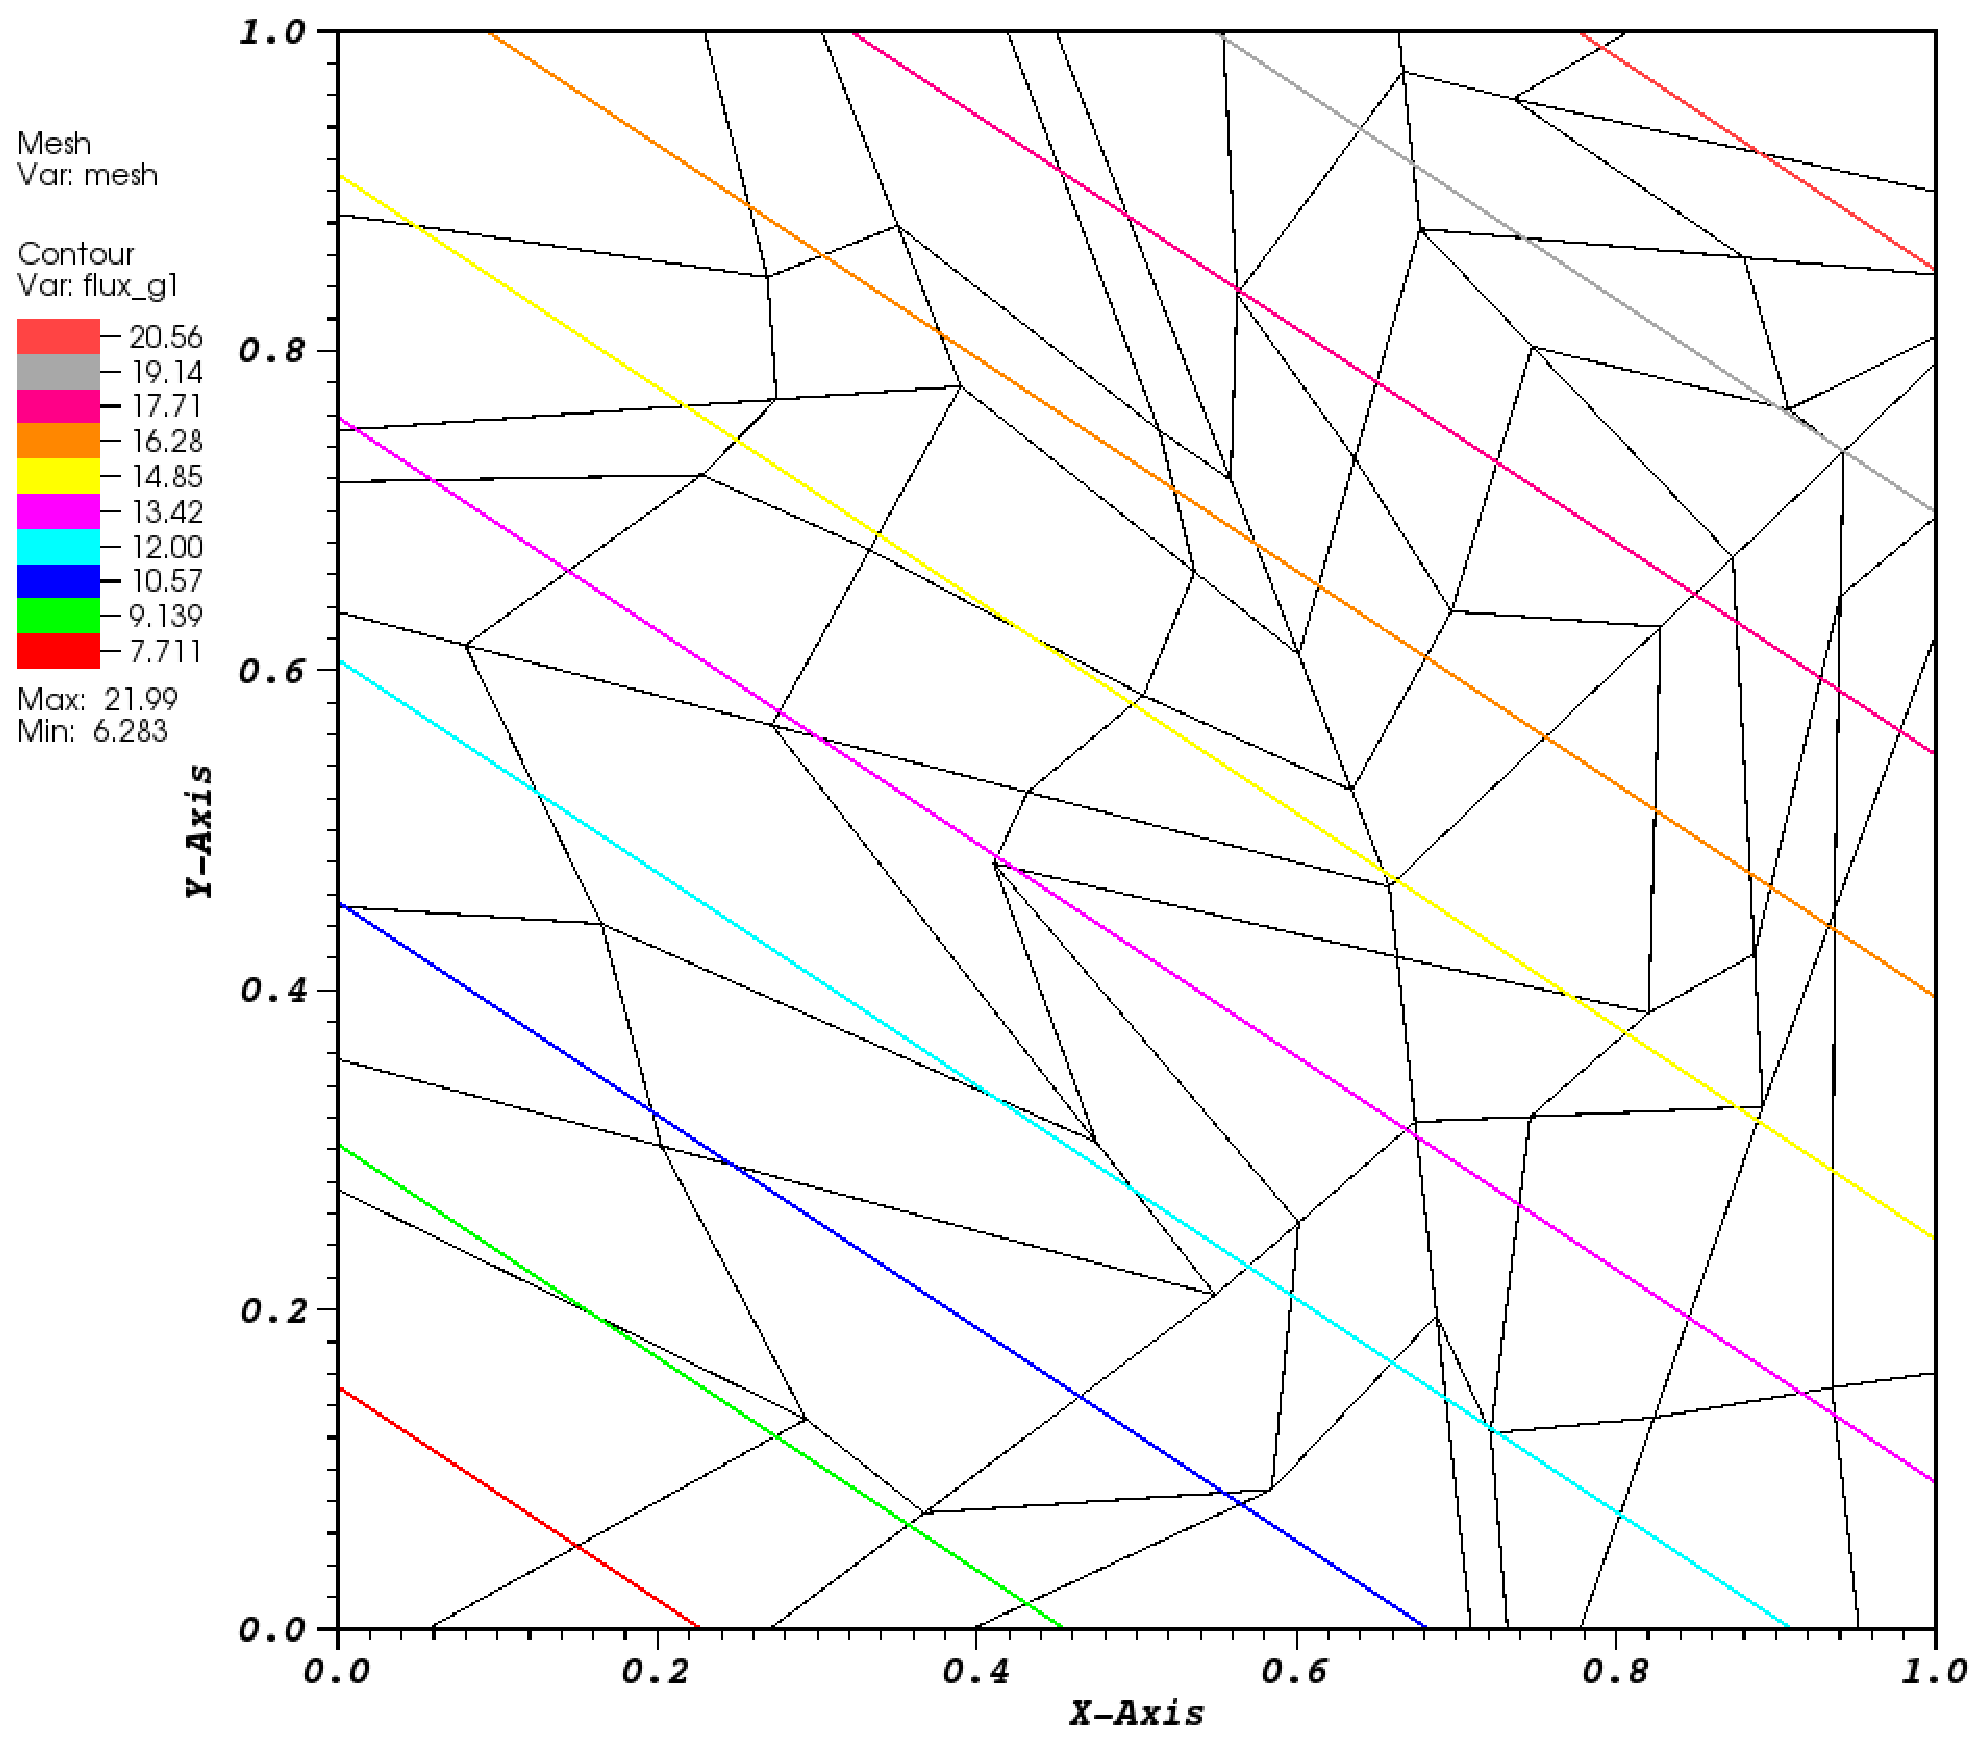
\includegraphics[width=\textwidth]{figures/sec_BF/shes_quad_MV_k1.eps}
		\caption{}
	\end{subfigure}
	\hfill
	\begin{subfigure}[b]{0.45\textwidth}
		\centering
		\label{subfig::smooth_poly_mv_lin_sol}
		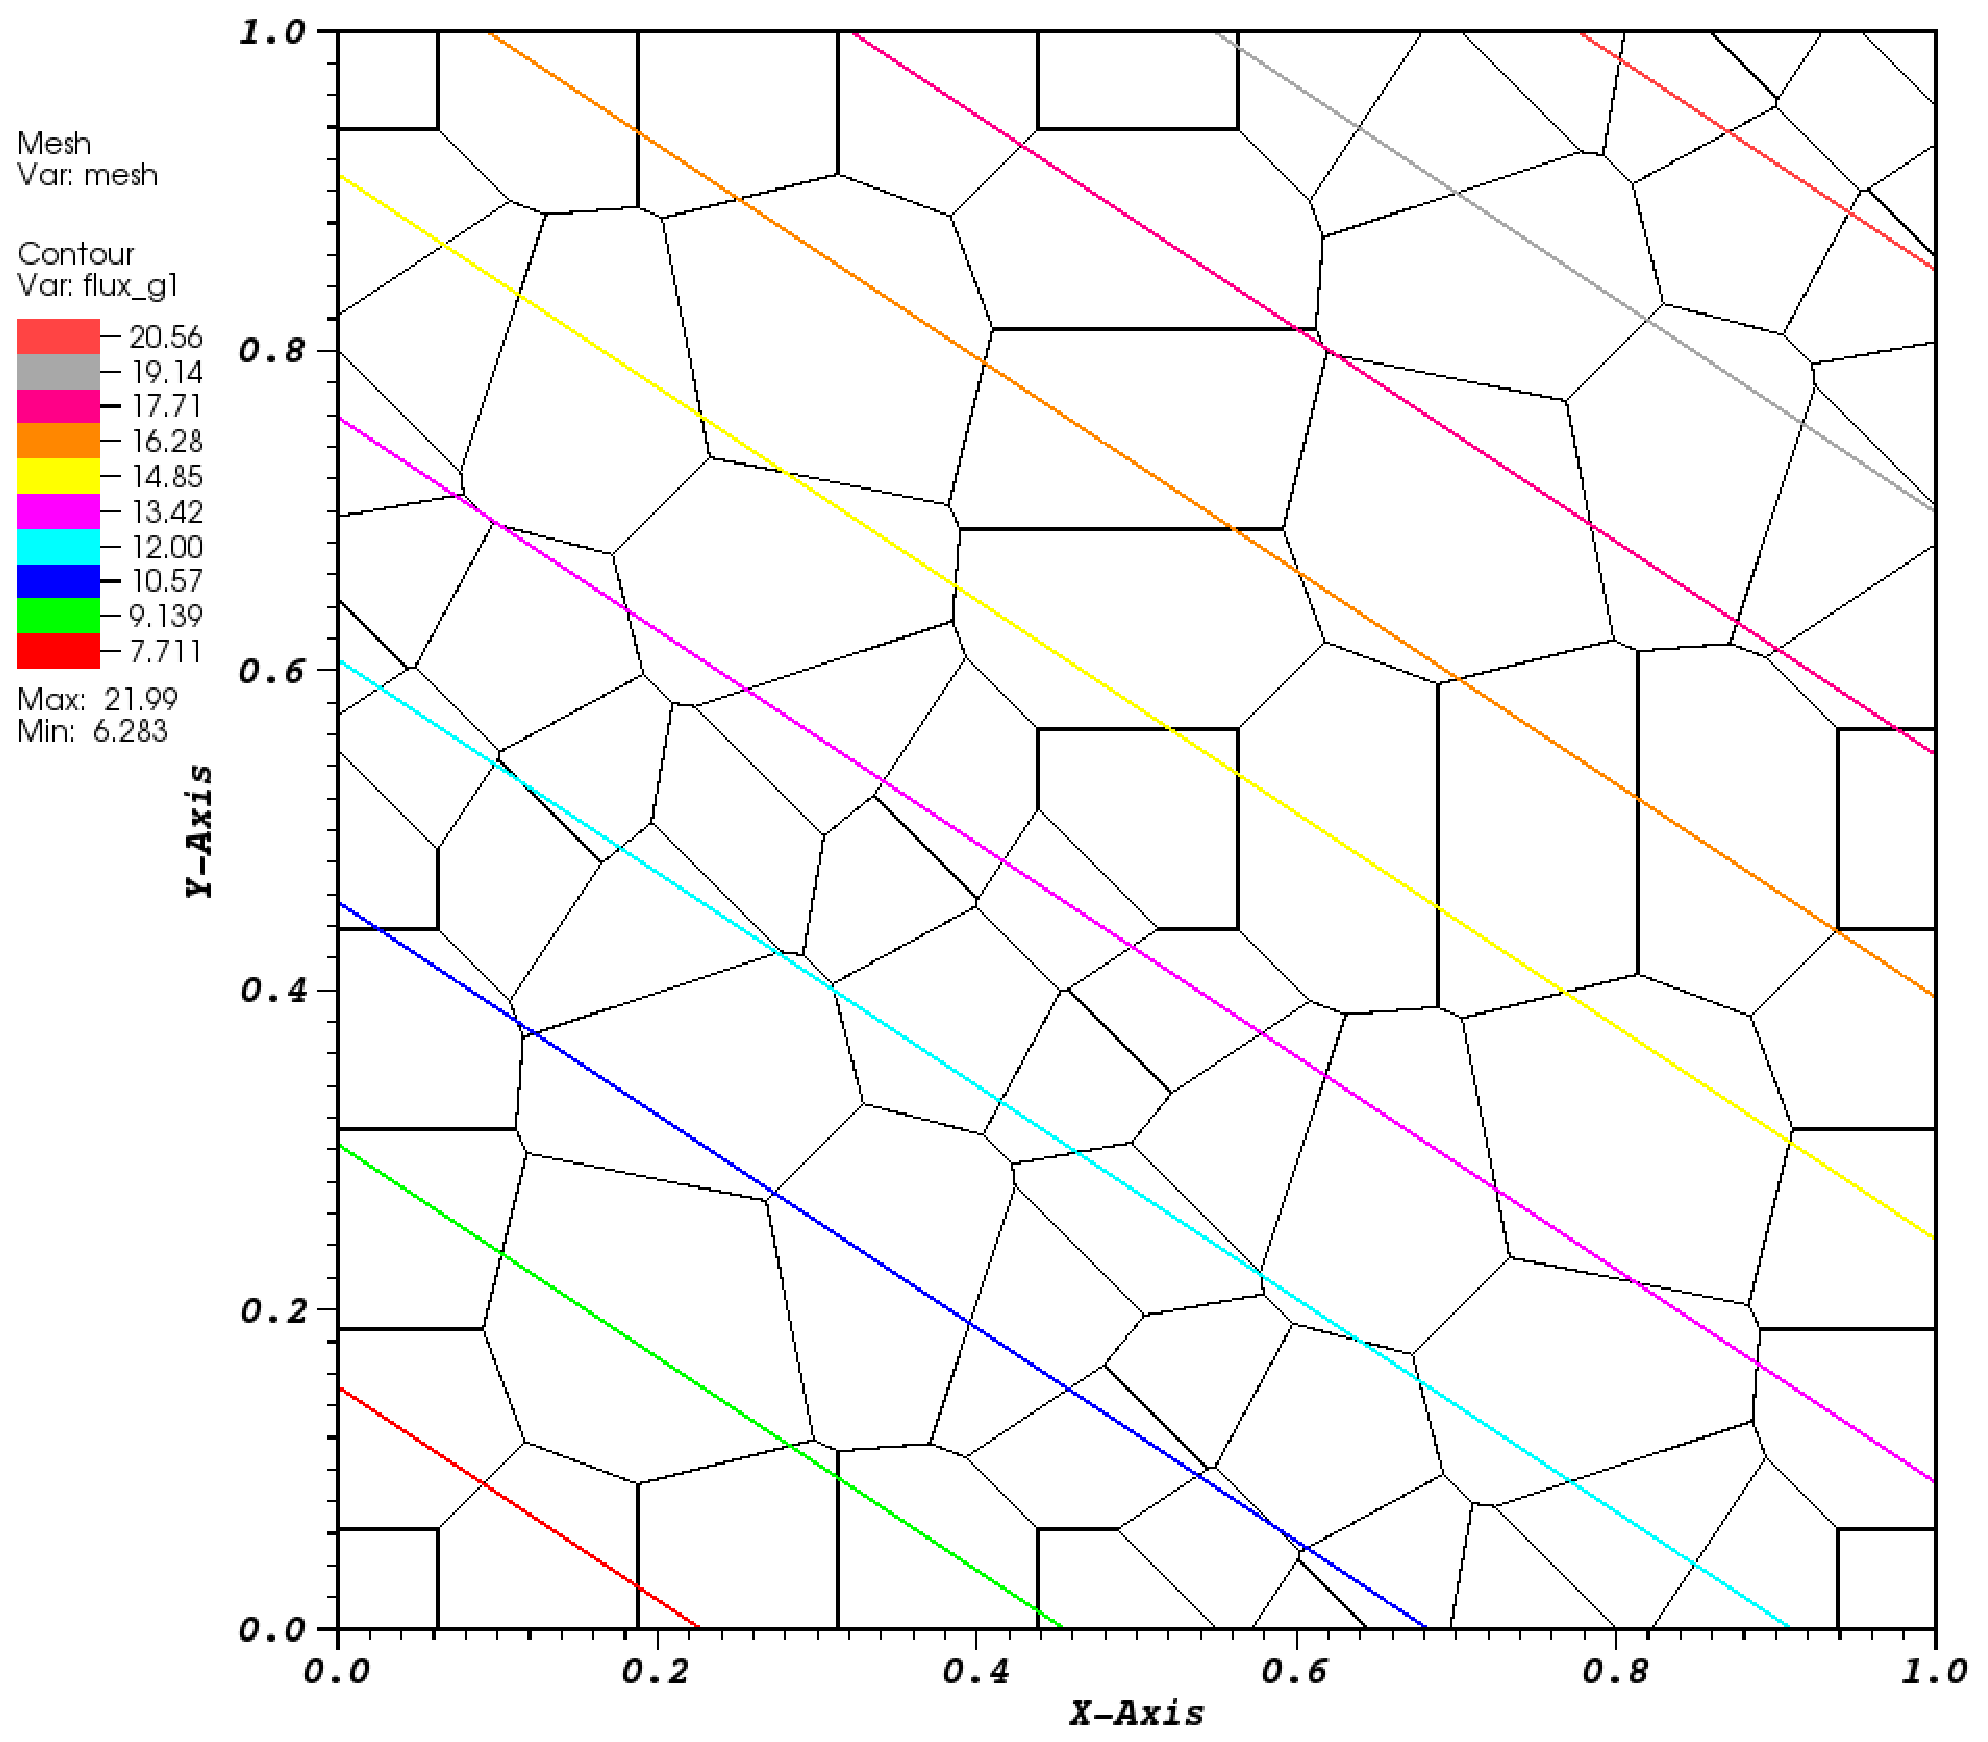
\includegraphics[width=\textwidth]{figures/sec_BF/smooth_poly_MV_k1.eps}
		\caption{}
	\end{subfigure}
	\vfill
	\begin{subfigure}[b]{0.45\textwidth}
		\centering
		\label{subfig::z_quad_mv_lin_sol}
		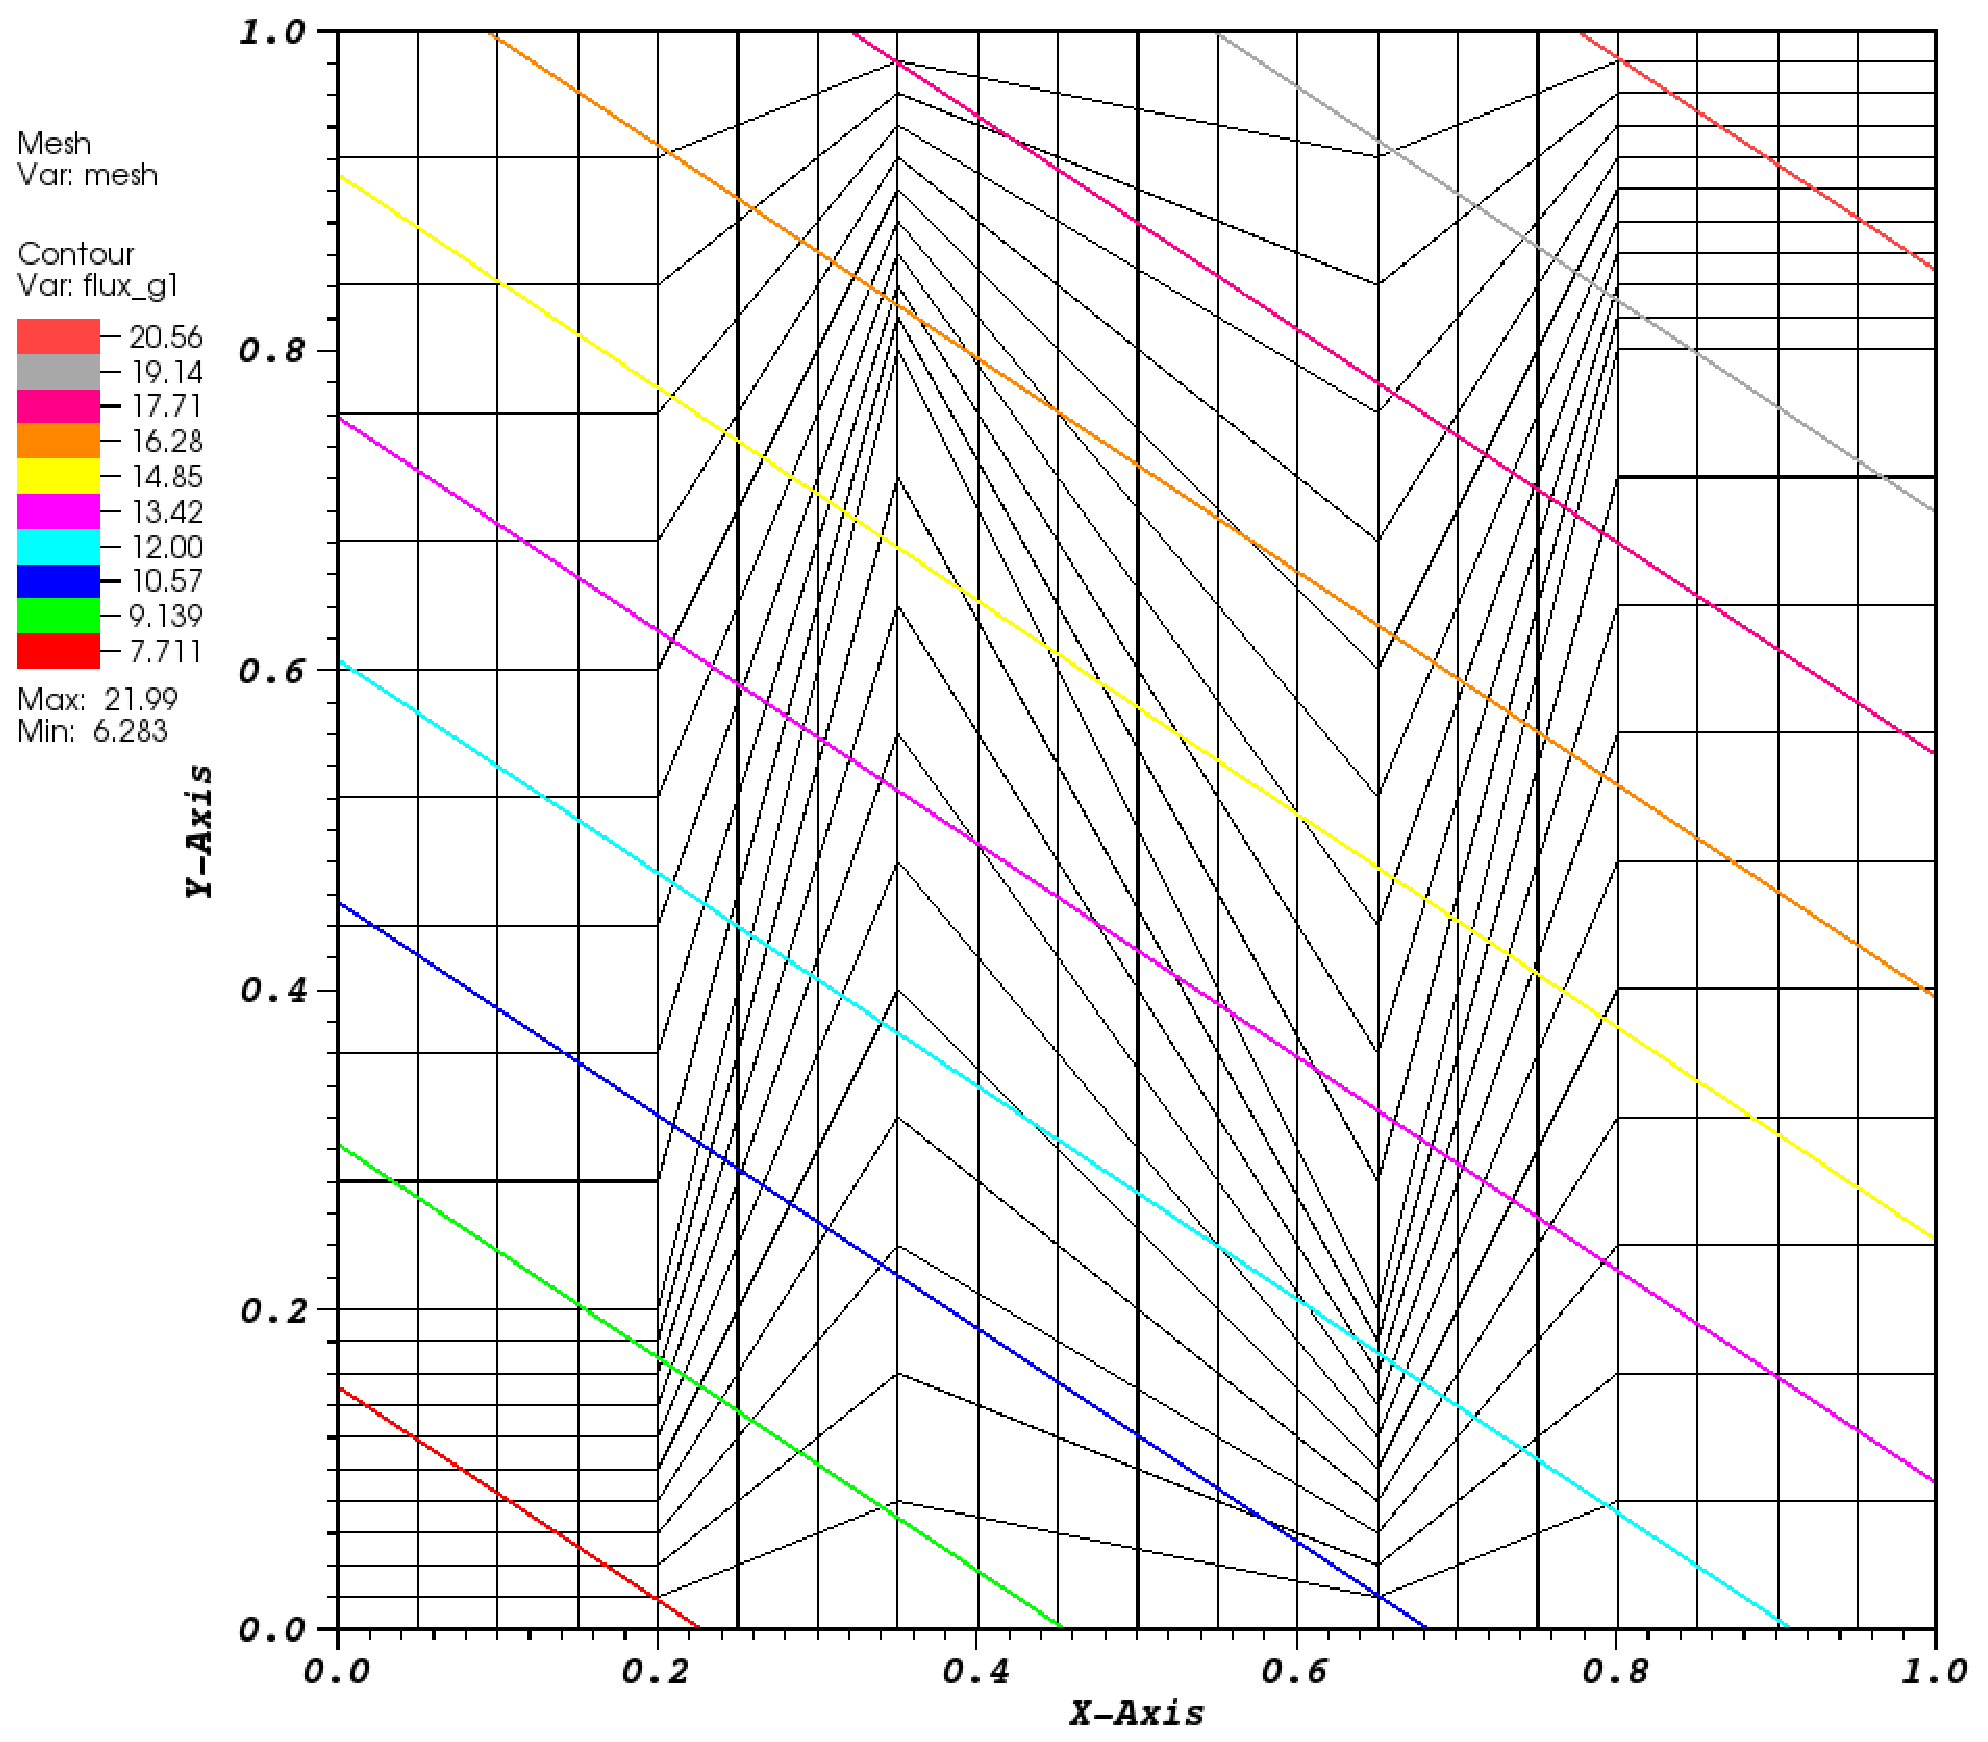
\includegraphics[width=\textwidth]{figures/sec_BF/z_quad_MV_k1.eps}
		\caption{}
	\end{subfigure}
	\hfill
	\begin{subfigure}[b]{0.45\textwidth}
		\centering
		\label{subfig::z_poly_mv_lin_sol}
		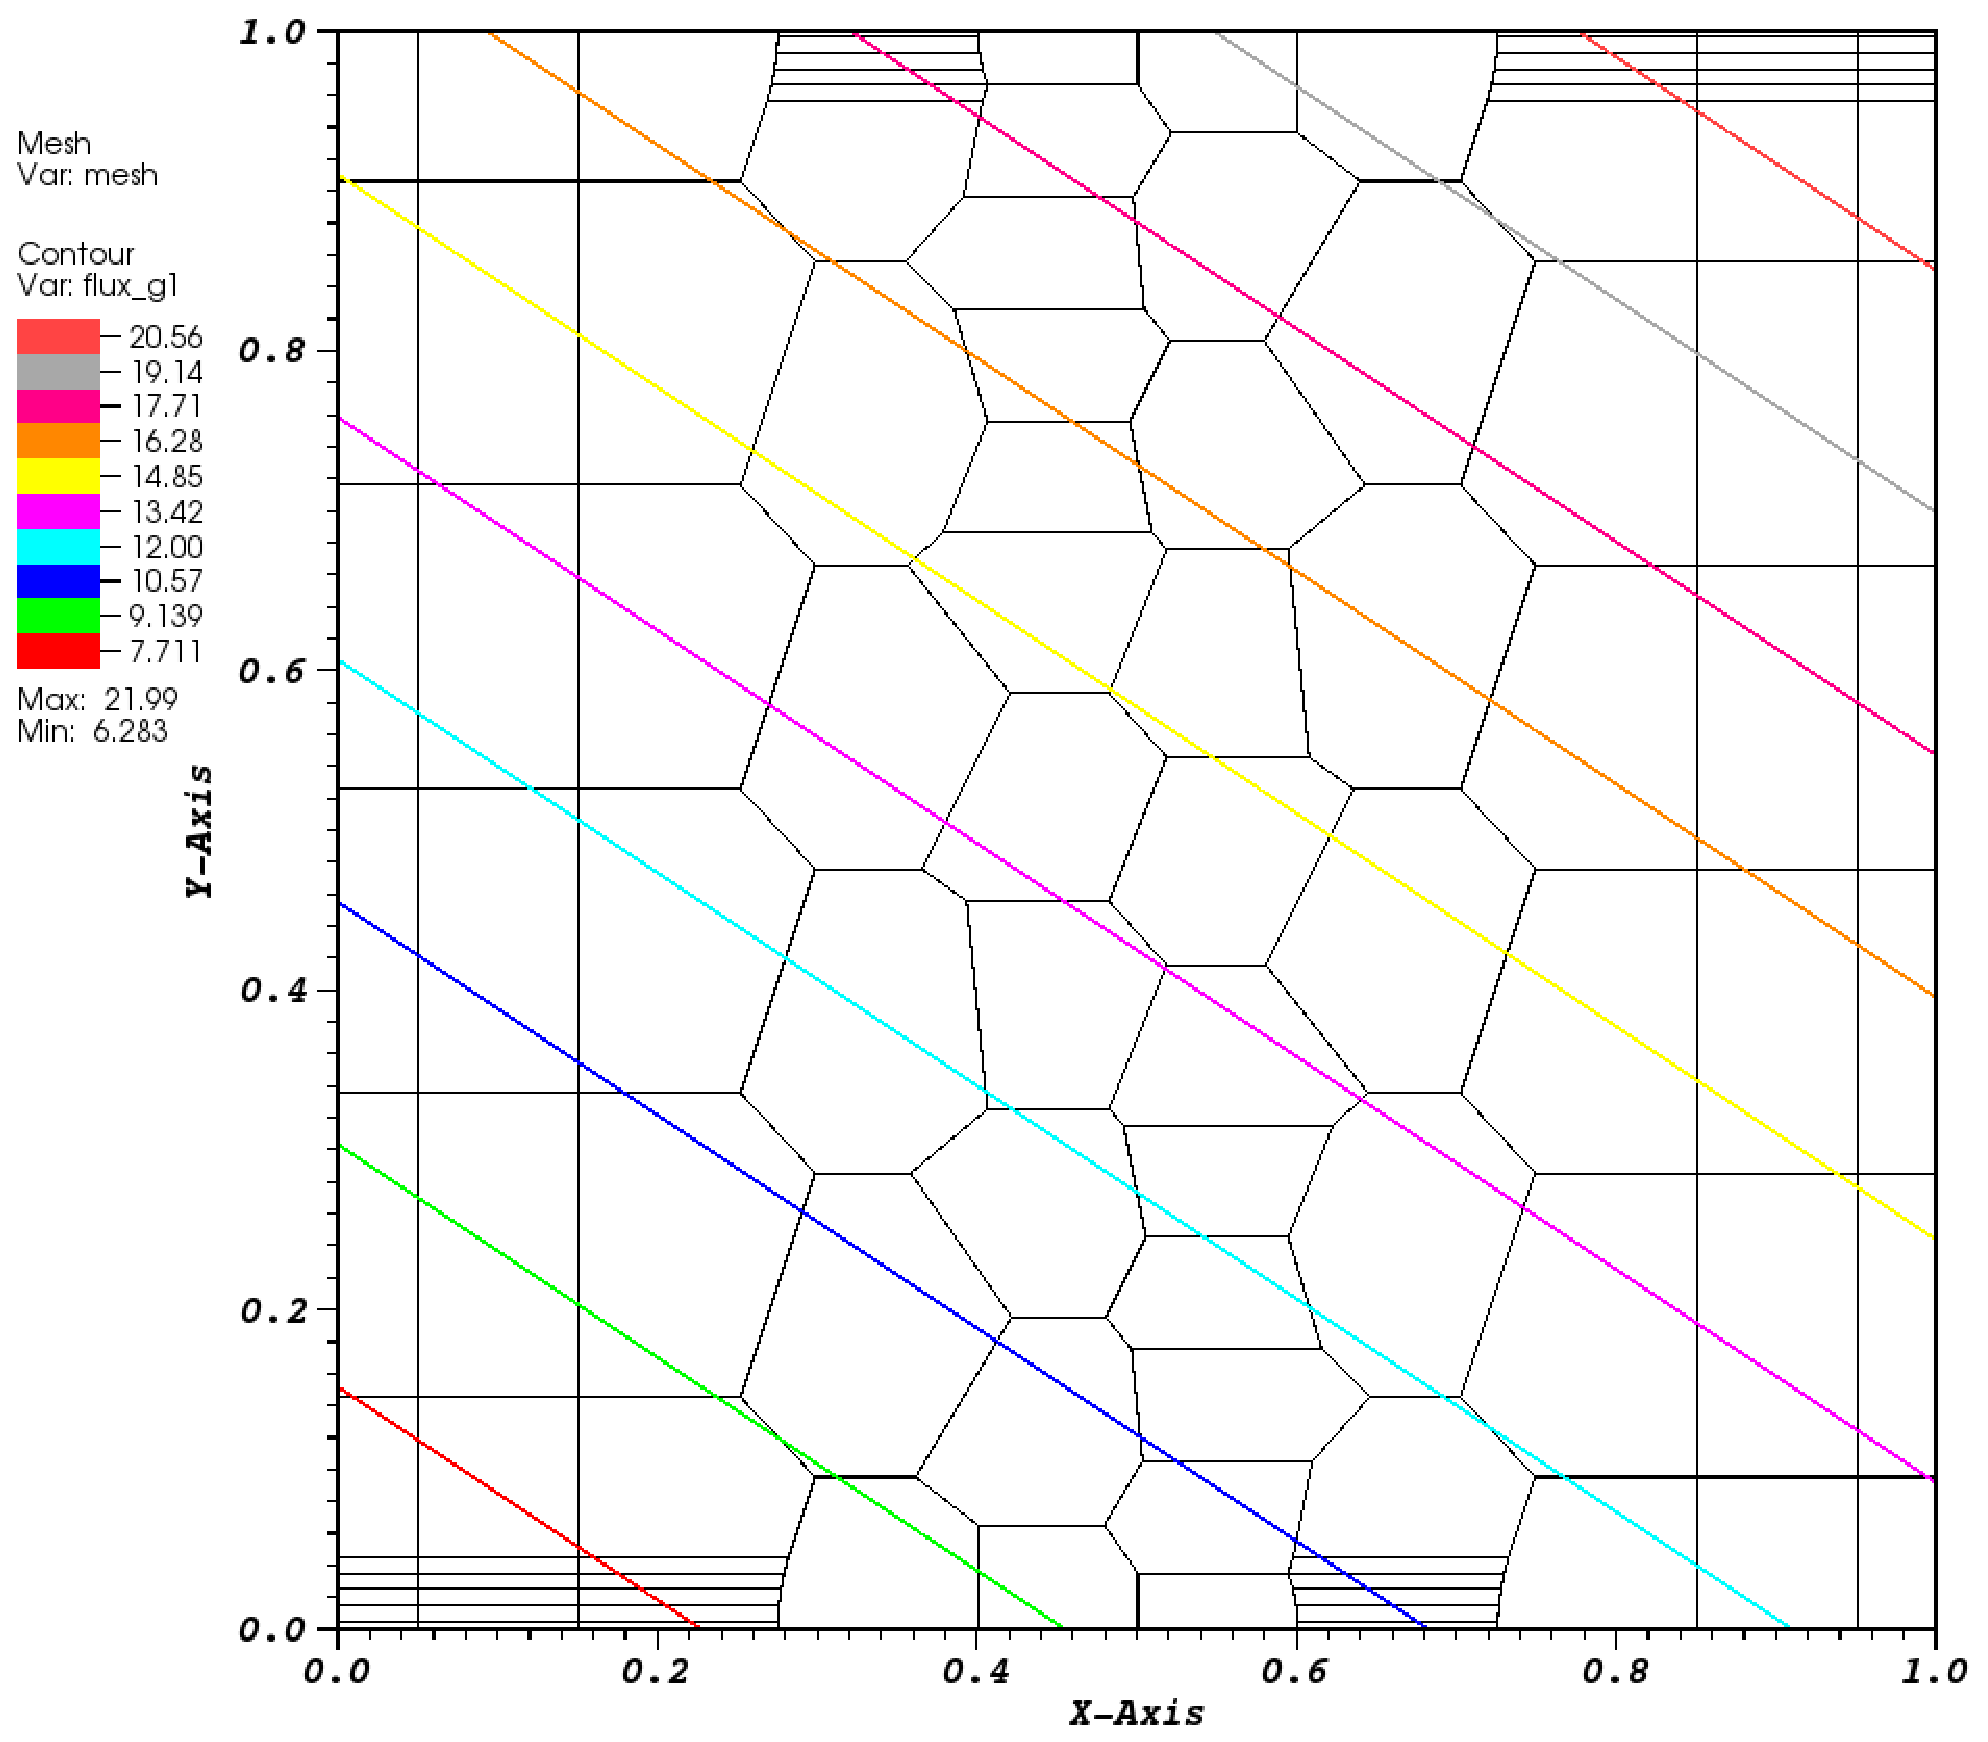
\includegraphics[width=\textwidth]{figures/sec_BF/z_poly_MV_k1.eps}
		\caption{}
	\end{subfigure}
\caption{Contour plots of the exactly-linear solution with the mean value basis functions on (a) cartesian mesh, (b) ordered-triangular mesh, (c) quadrilateral shestakov mesh, (d) sinusoidal polygonal mesh, (e) quadrilateral z-mesh, and (f) polygonal z-mesh.}
\label{fig::BF_Results_Linear_mv_sol}
\end{figure}

\begin{figure}
\centering
	\begin{subfigure}[b]{0.45\textwidth}
		\centering
		\label{subfig::cart_me_k1_lin_sol}
		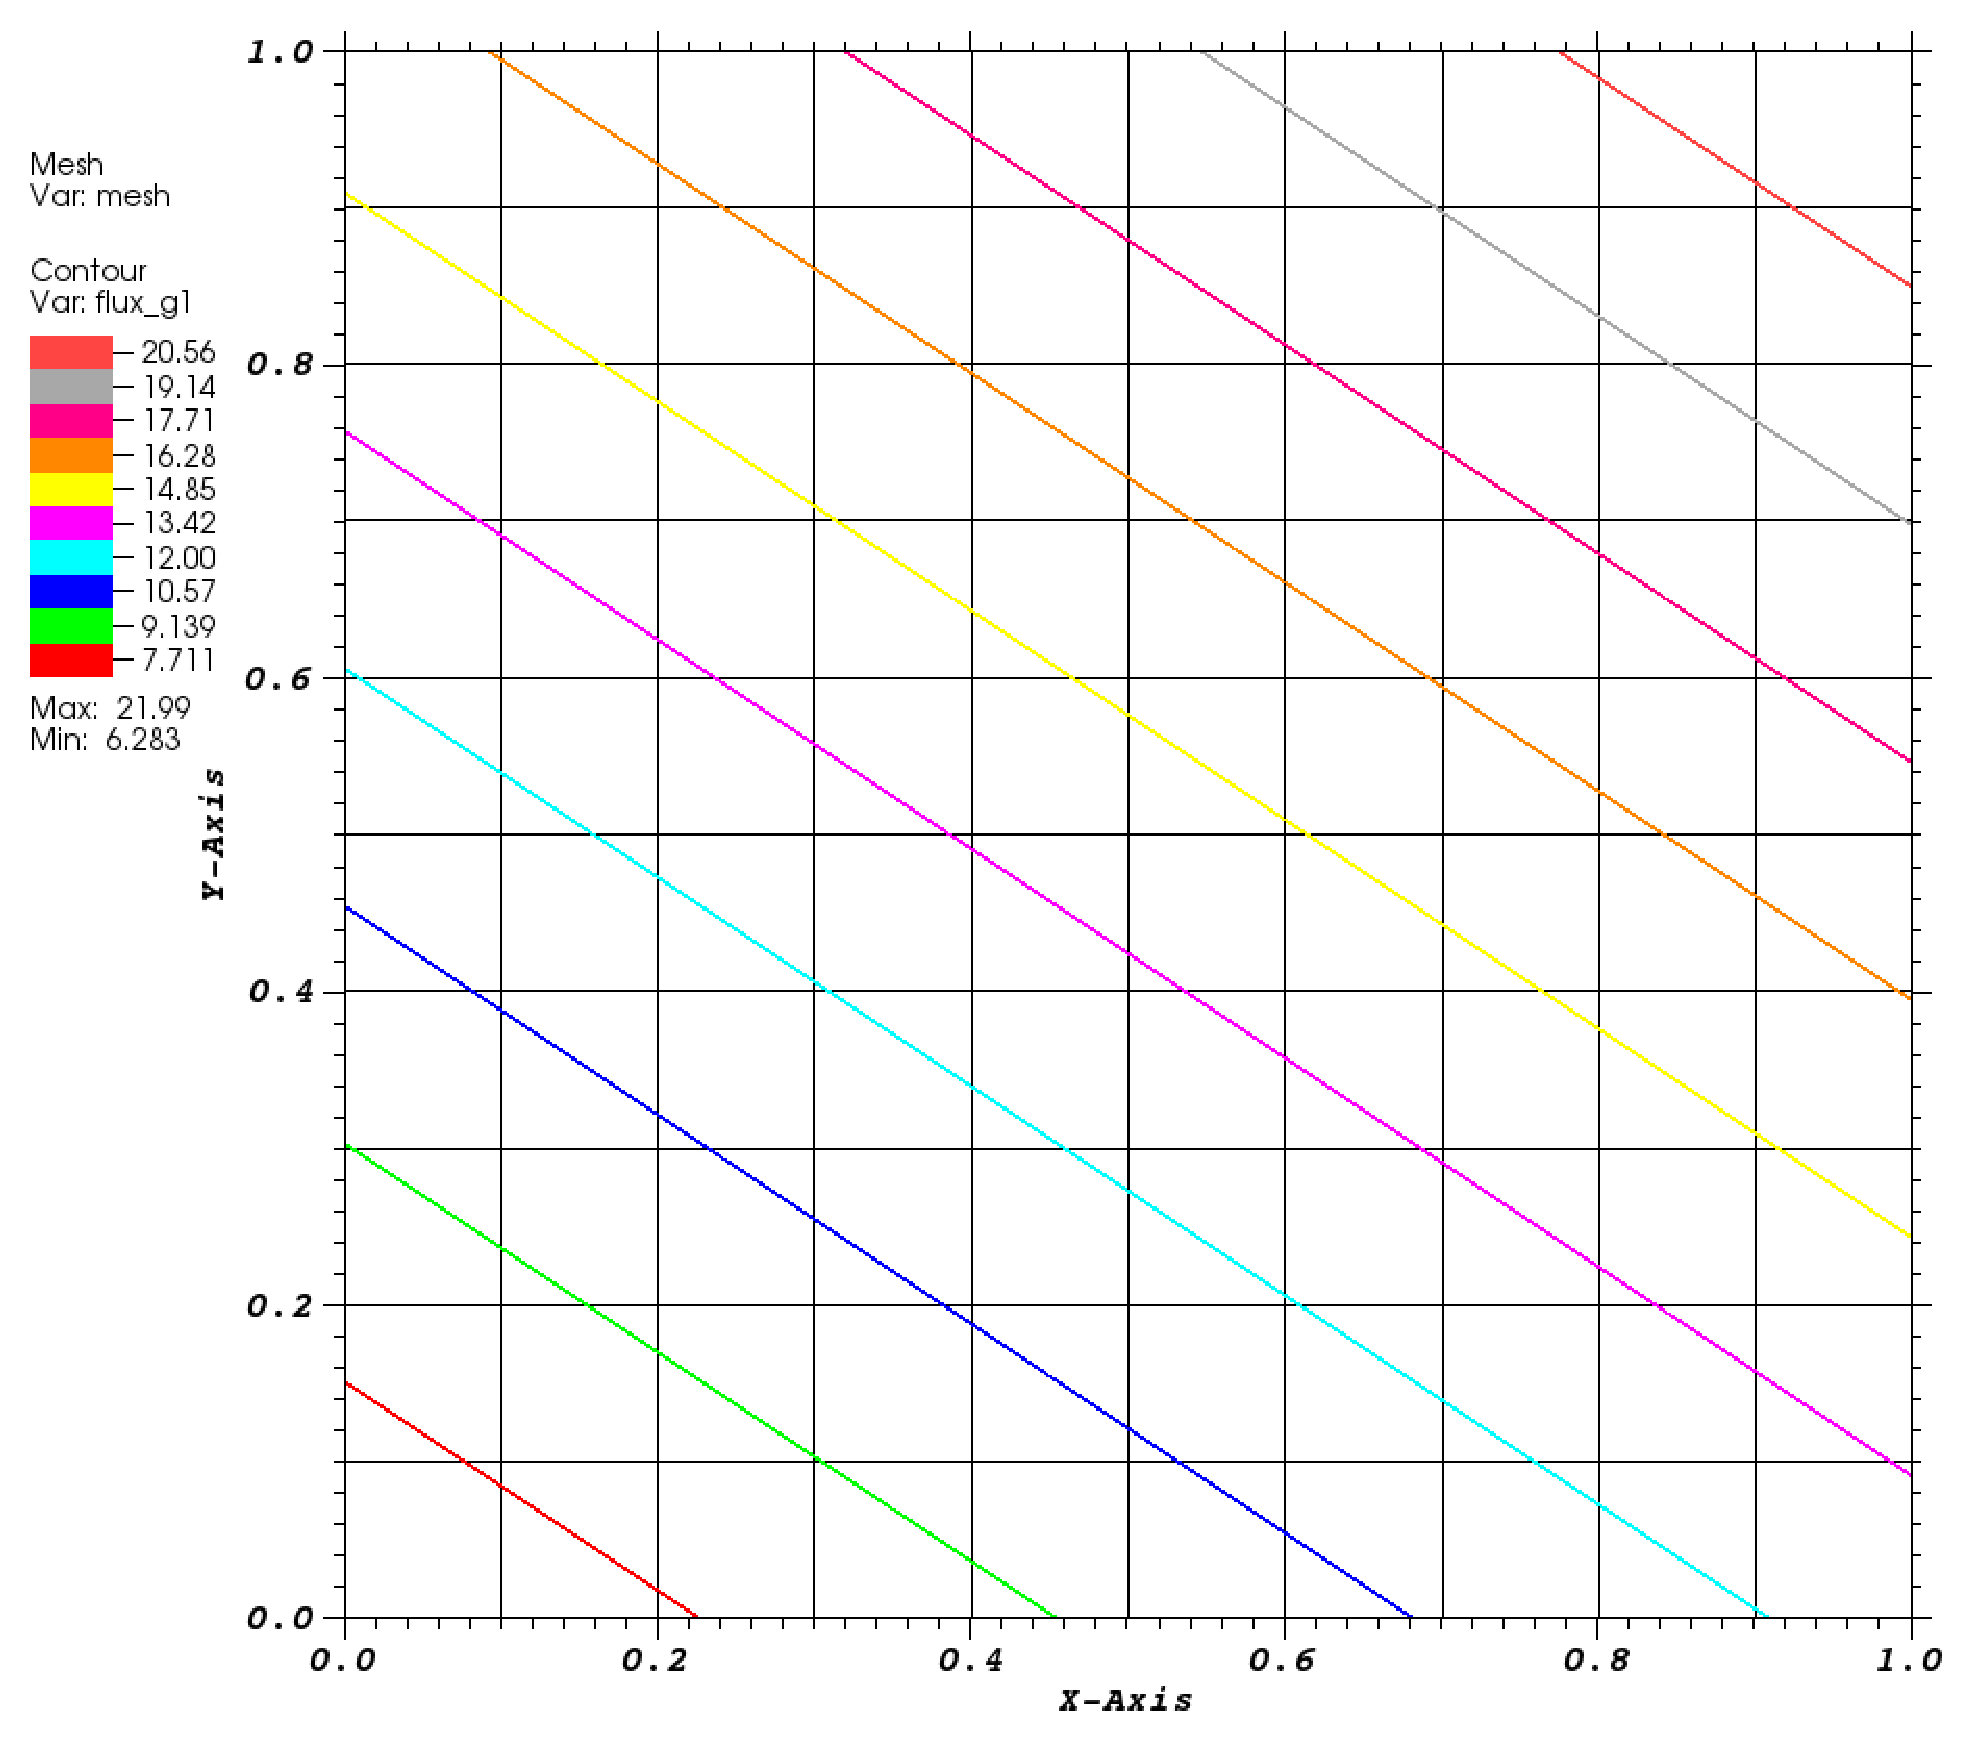
\includegraphics[width=\textwidth]{figures/sec_BF/cart_MAXENT_k1.eps}
		\caption{}
	\end{subfigure}
	\hfill
	\begin{subfigure}[b]{0.45\textwidth}
		\centering
		\label{subfig::tri_me_k1_lin_sol}
		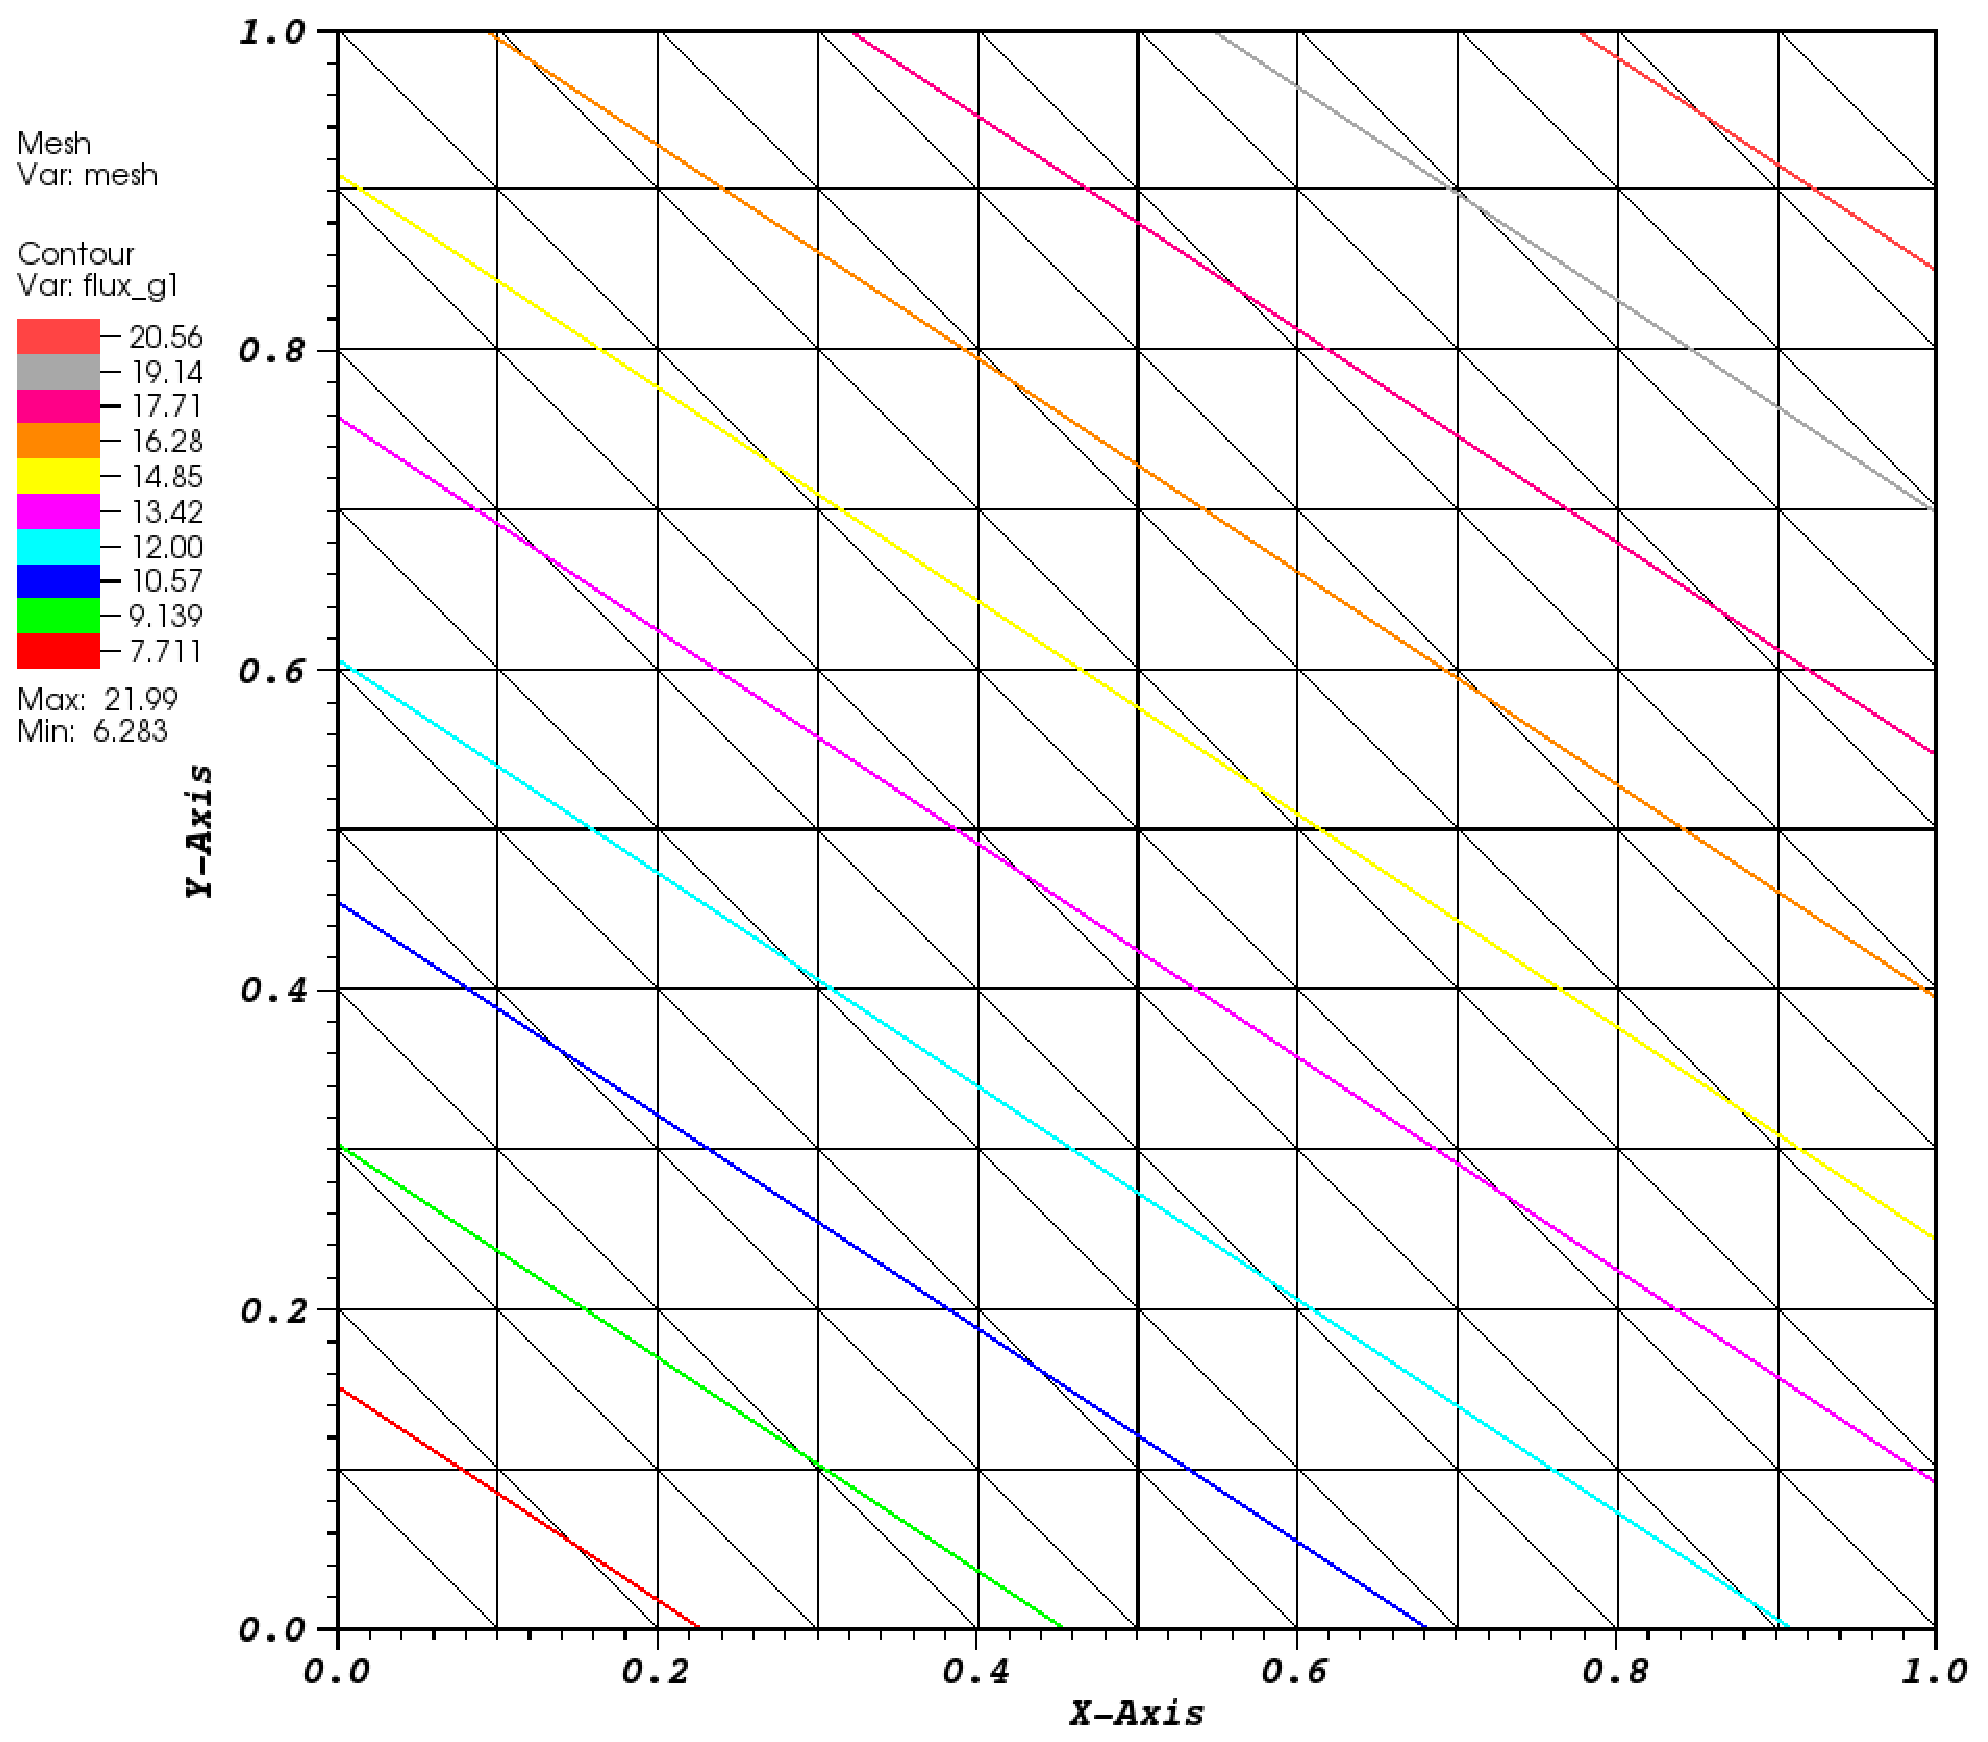
\includegraphics[width=\textwidth]{figures/sec_BF/tri_MAXENT_k1.eps}
		\caption{}
	\end{subfigure}
	\vfill
	\begin{subfigure}[b]{0.45\textwidth}
		\centering
		\label{subfig::shes_quad_me_k1_lin_sol}
		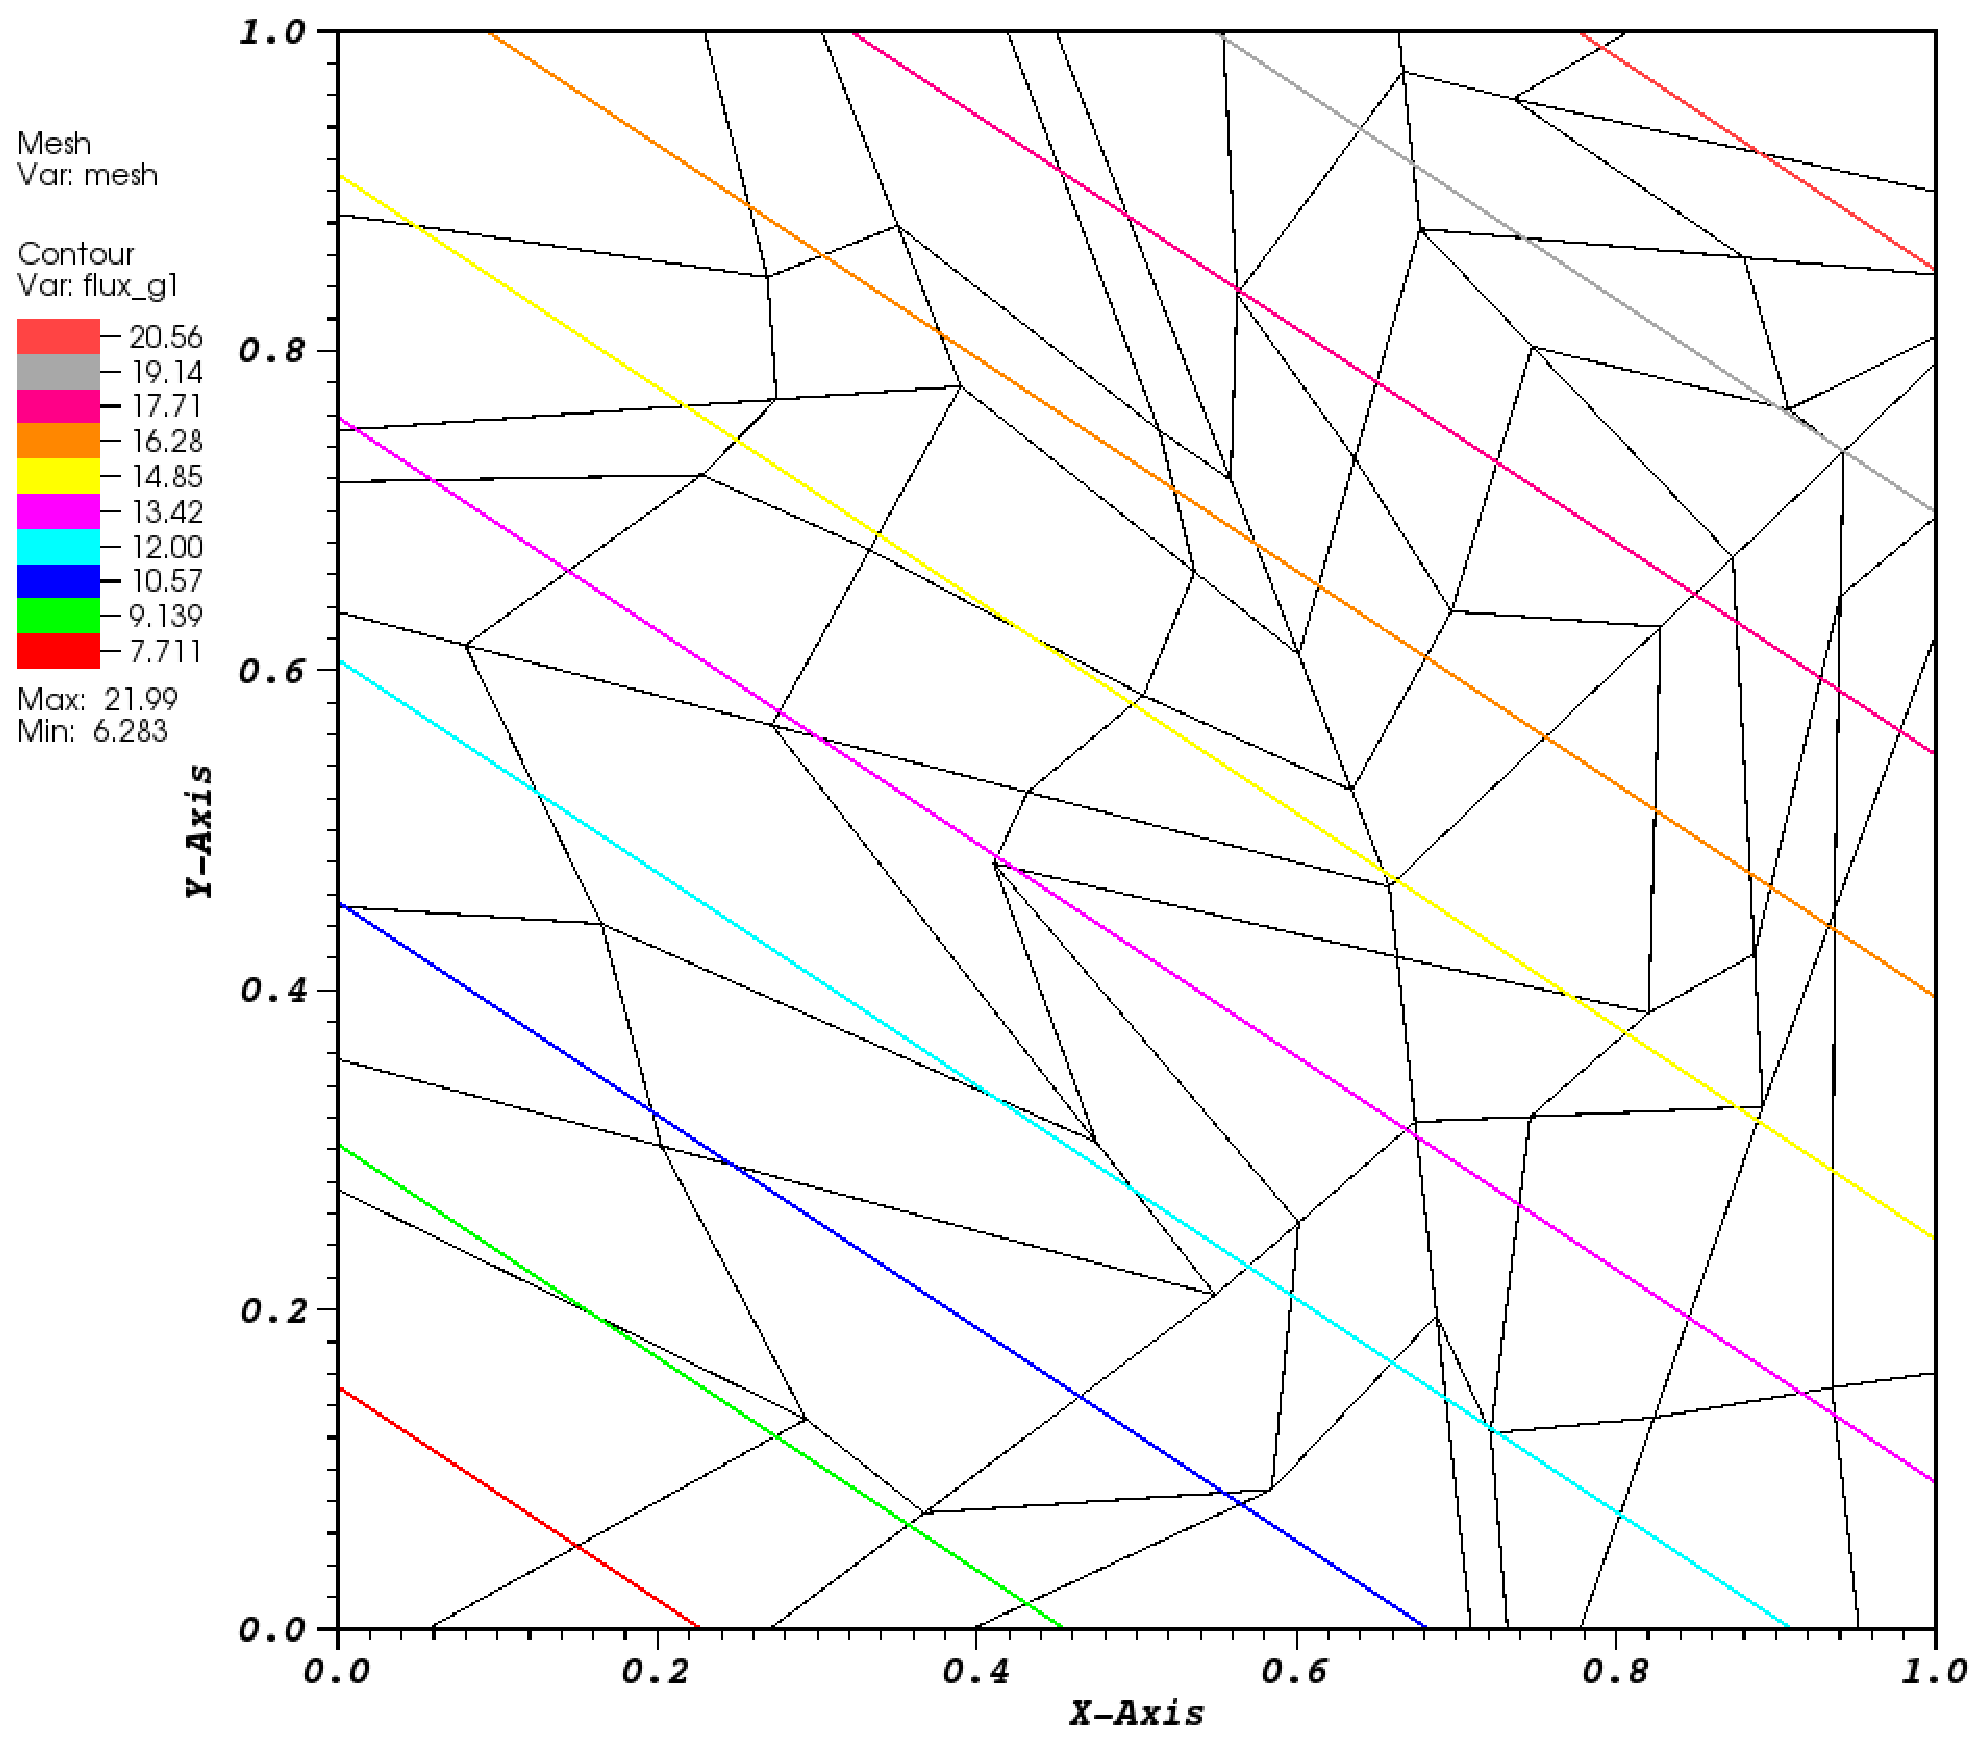
\includegraphics[width=\textwidth]{figures/sec_BF/shes_quad_MAXENT_k1.eps}
		\caption{}
	\end{subfigure}
	\hfill
	\begin{subfigure}[b]{0.45\textwidth}
		\centering
		\label{subfig::smooth_poly_me_k1_lin_sol}
		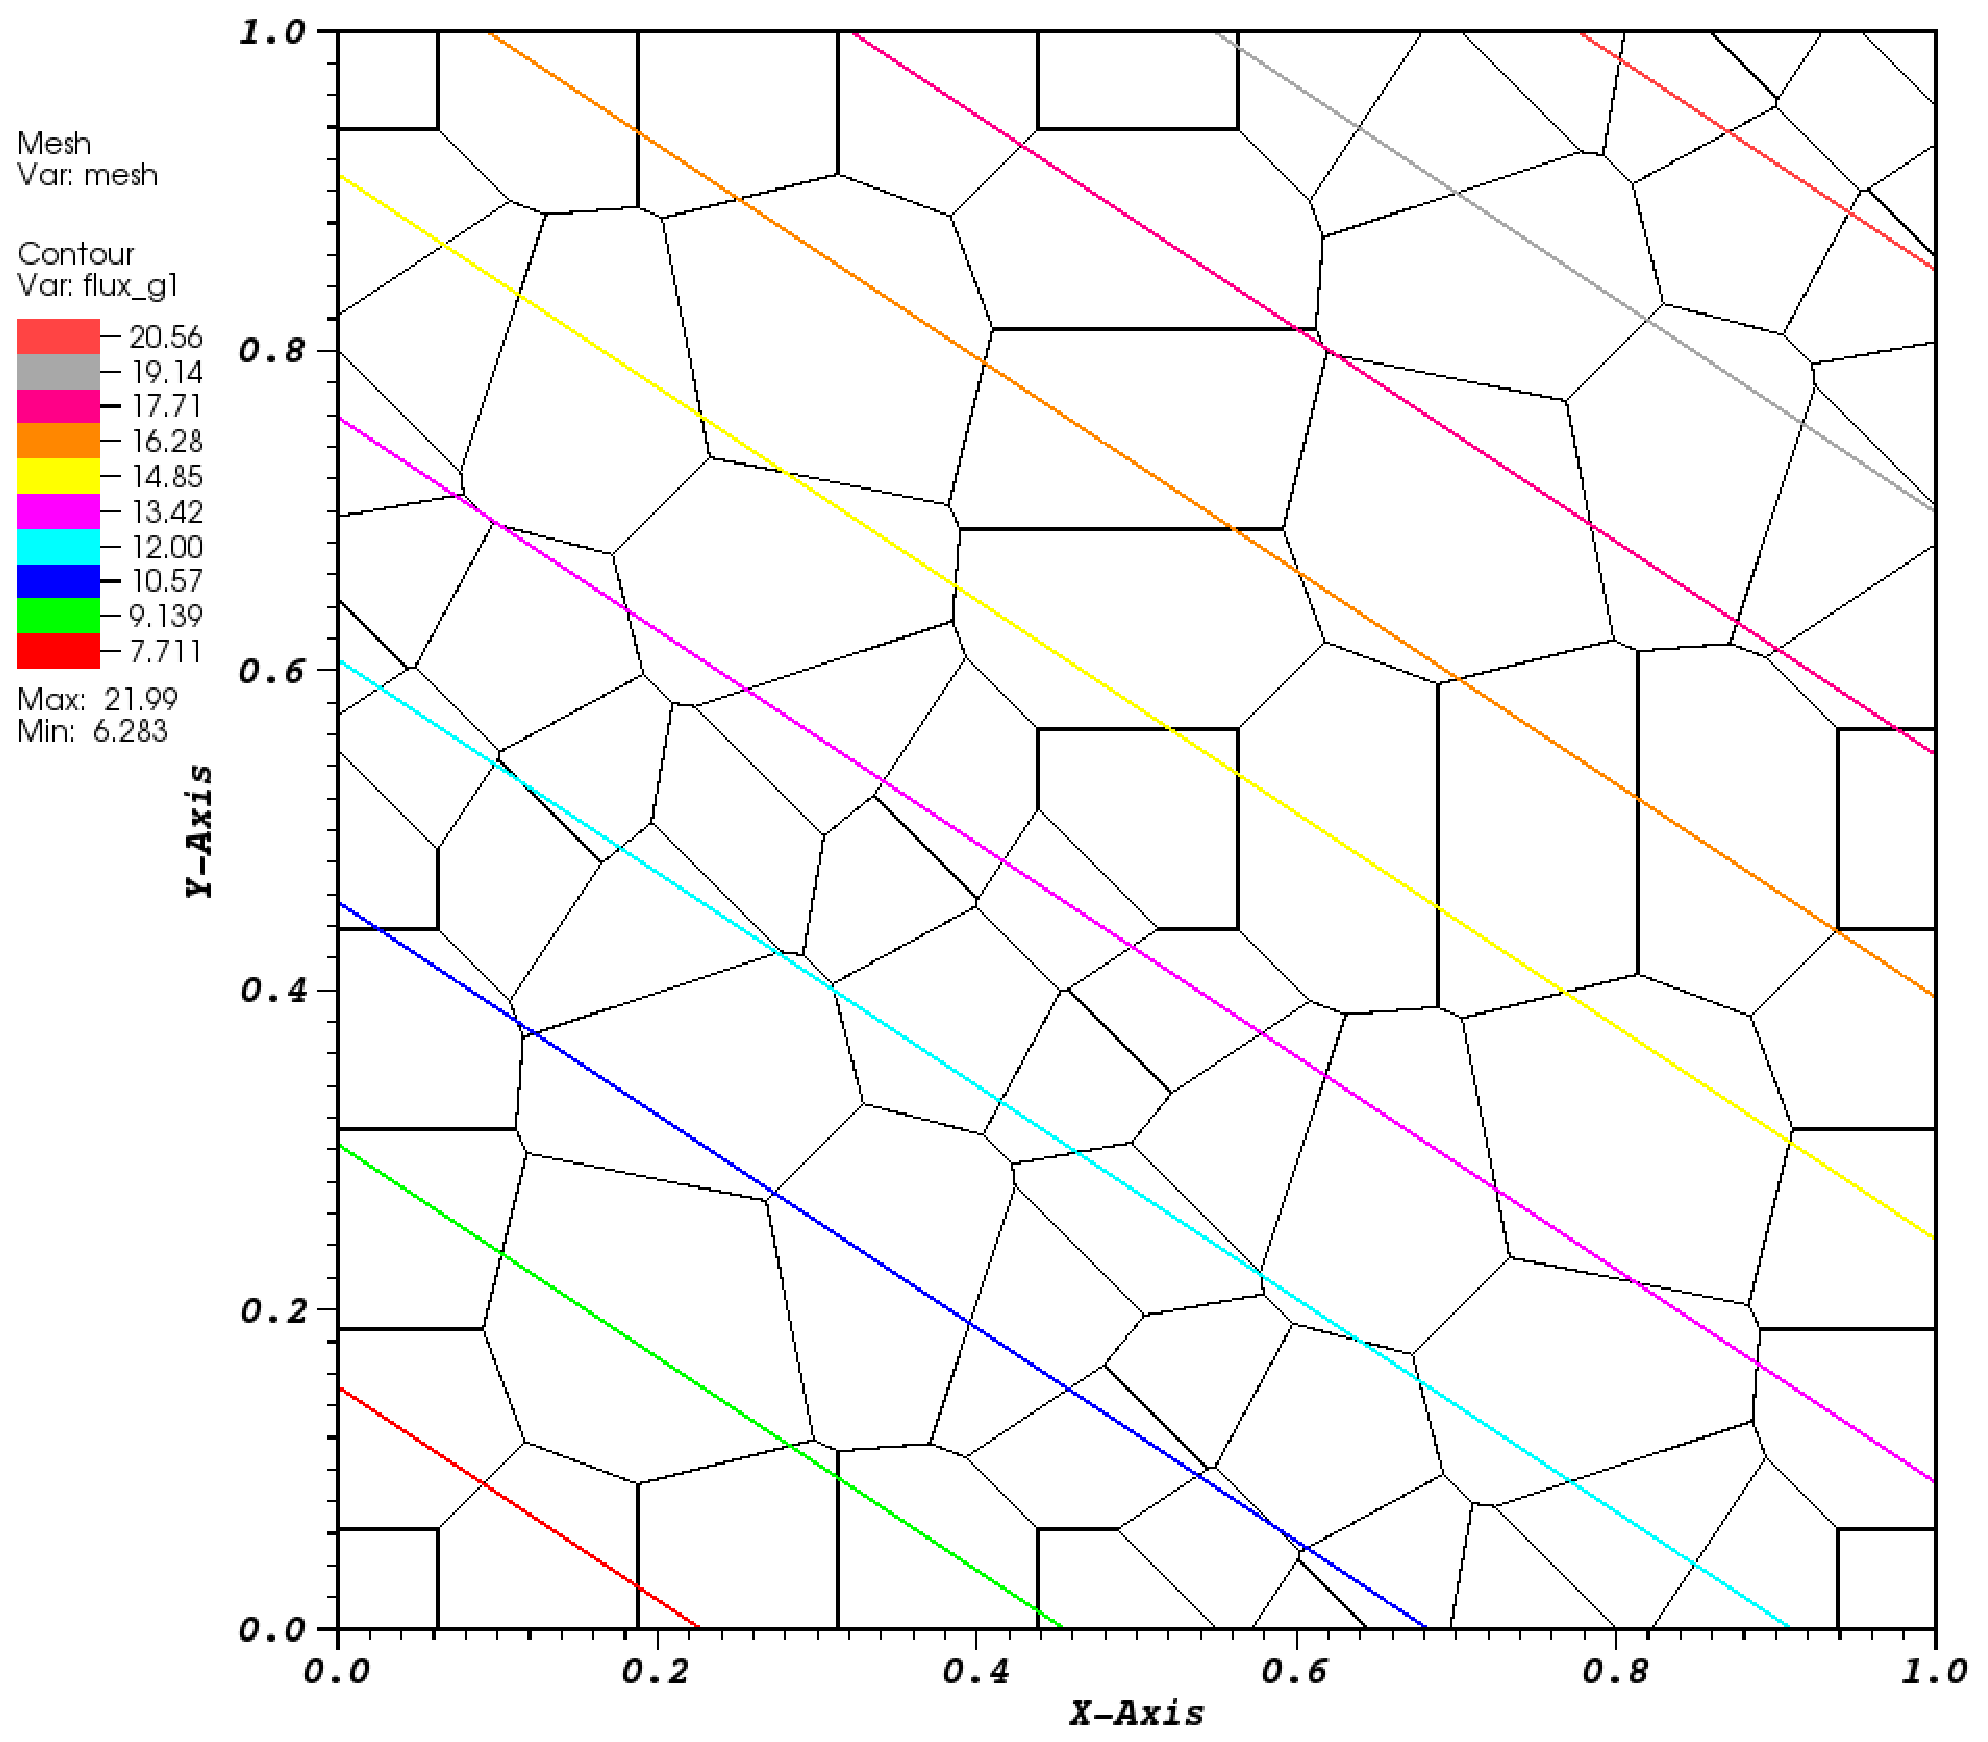
\includegraphics[width=\textwidth]{figures/sec_BF/smooth_poly_MAXENT_k1.eps}
		\caption{}
	\end{subfigure}
	\vfill
	\begin{subfigure}[b]{0.45\textwidth}
		\centering
		\label{subfig::z_quad_me_k1_lin_sol}
		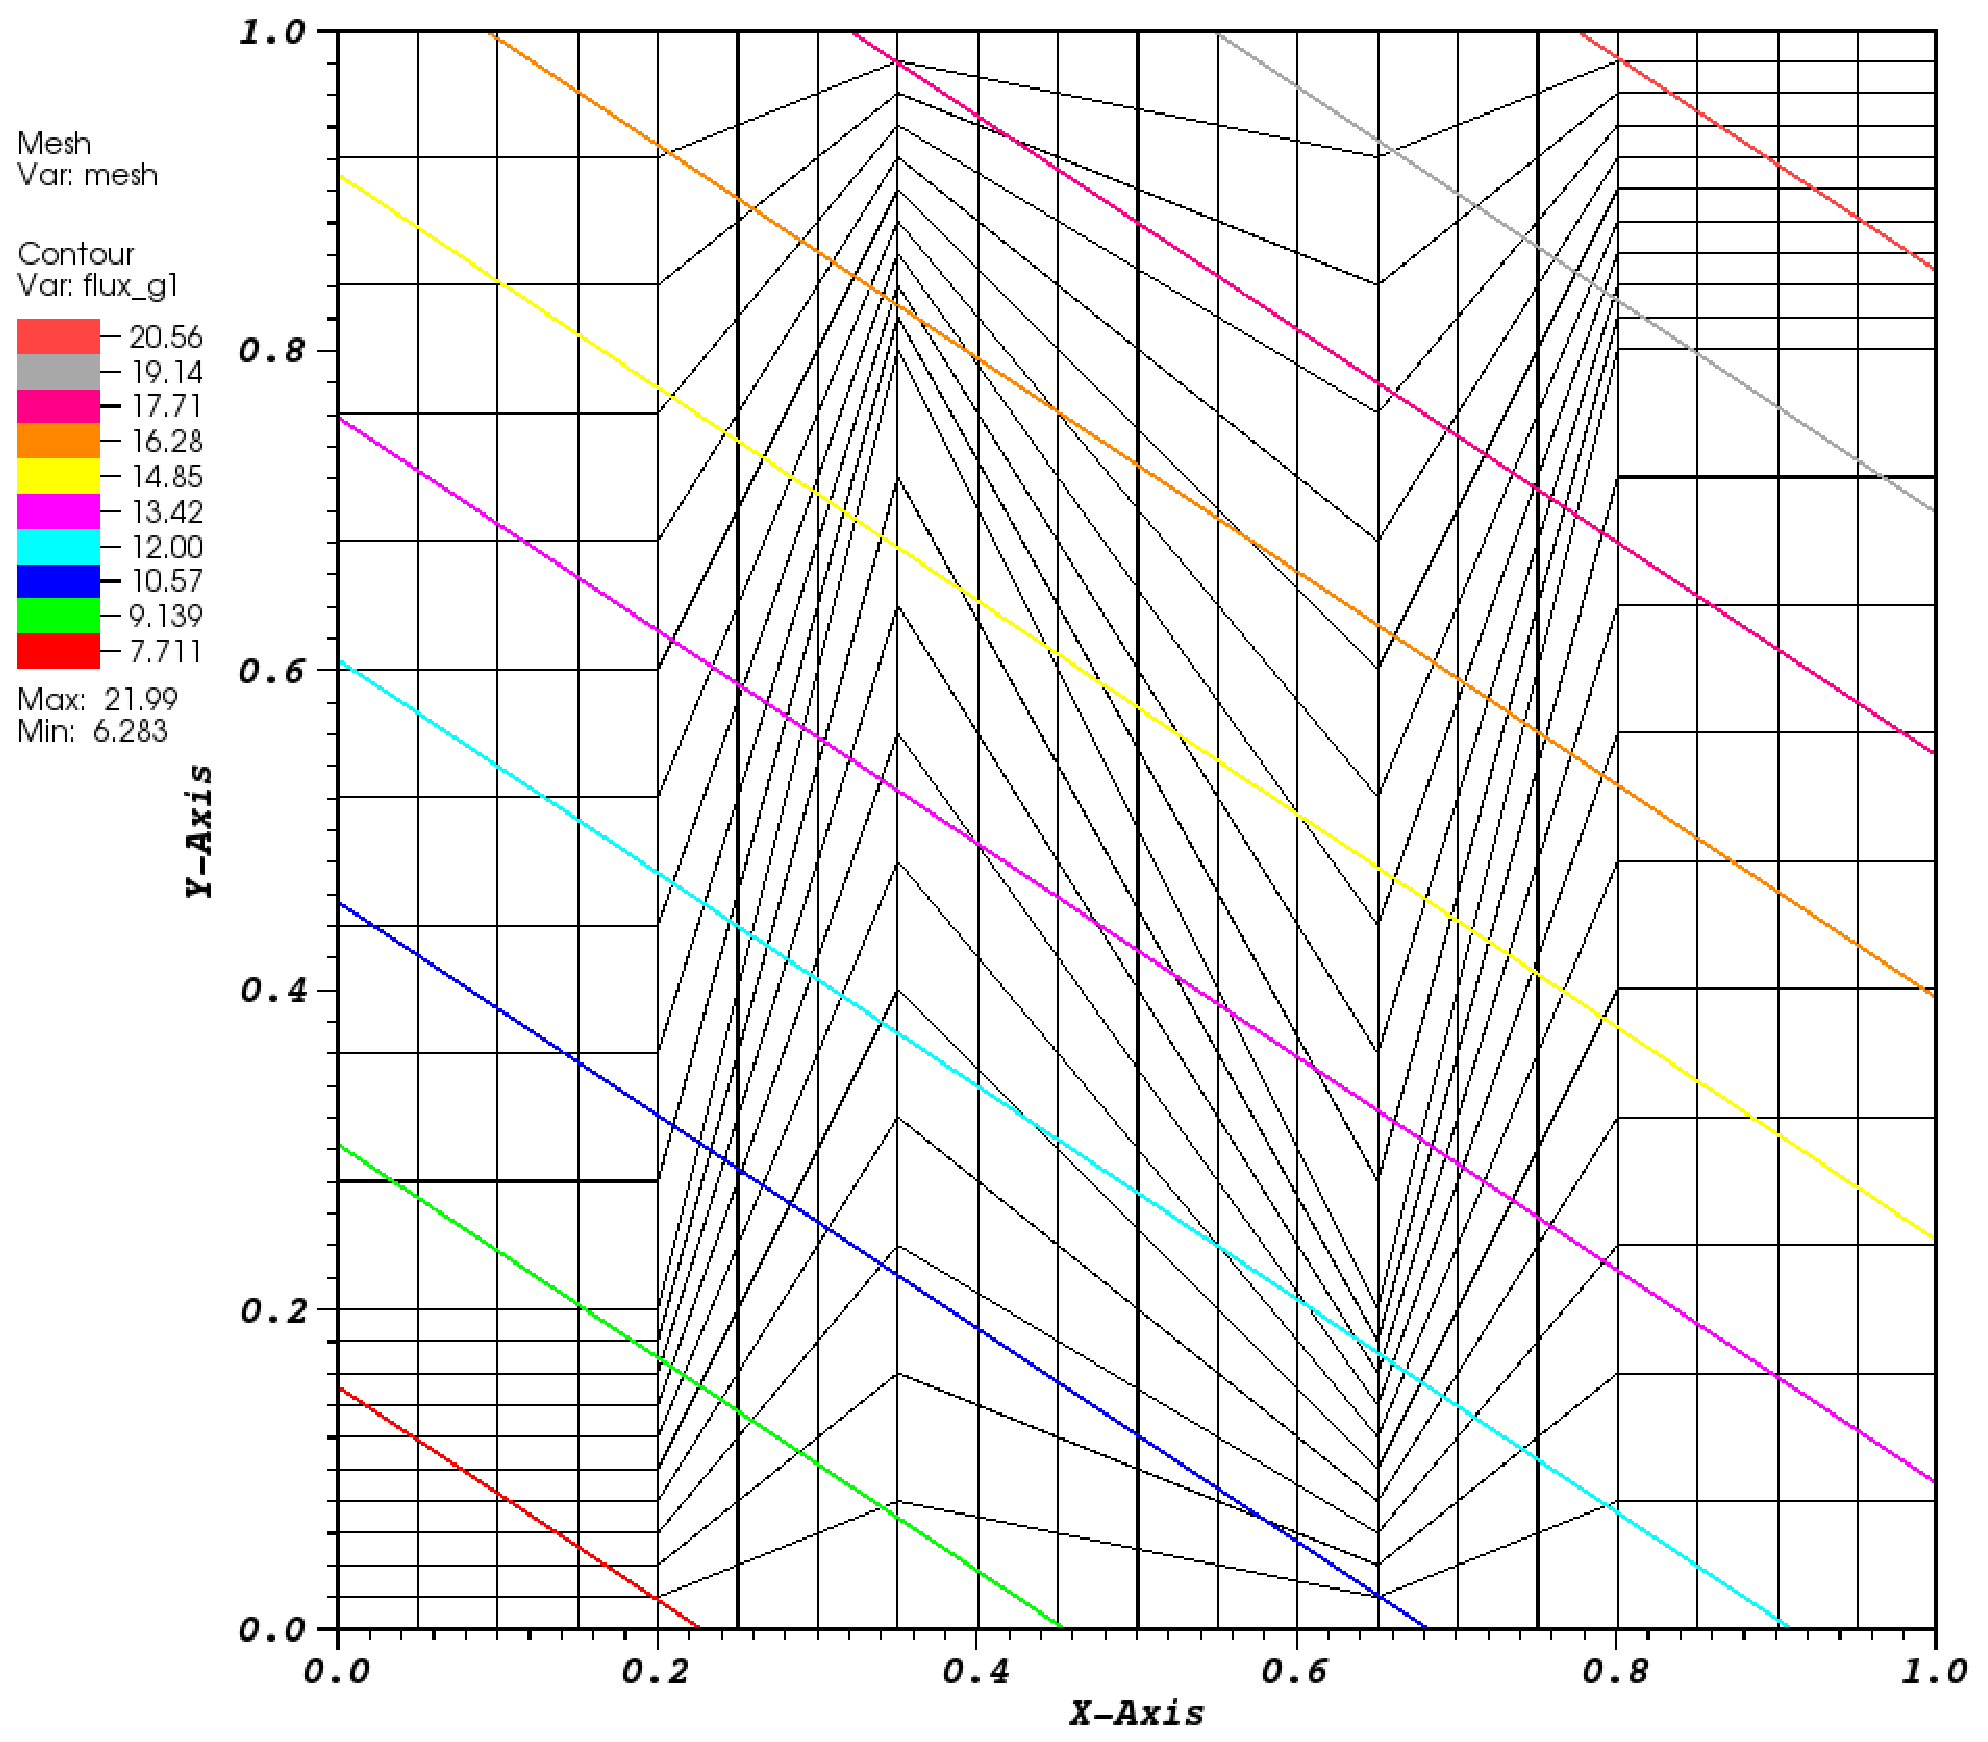
\includegraphics[width=\textwidth]{figures/sec_BF/z_quad_MAXENT_k1.eps}
		\caption{}
	\end{subfigure}
	\hfill
	\begin{subfigure}[b]{0.45\textwidth}
		\centering
		\label{subfig::z_poly_me_k1_lin_sol}
		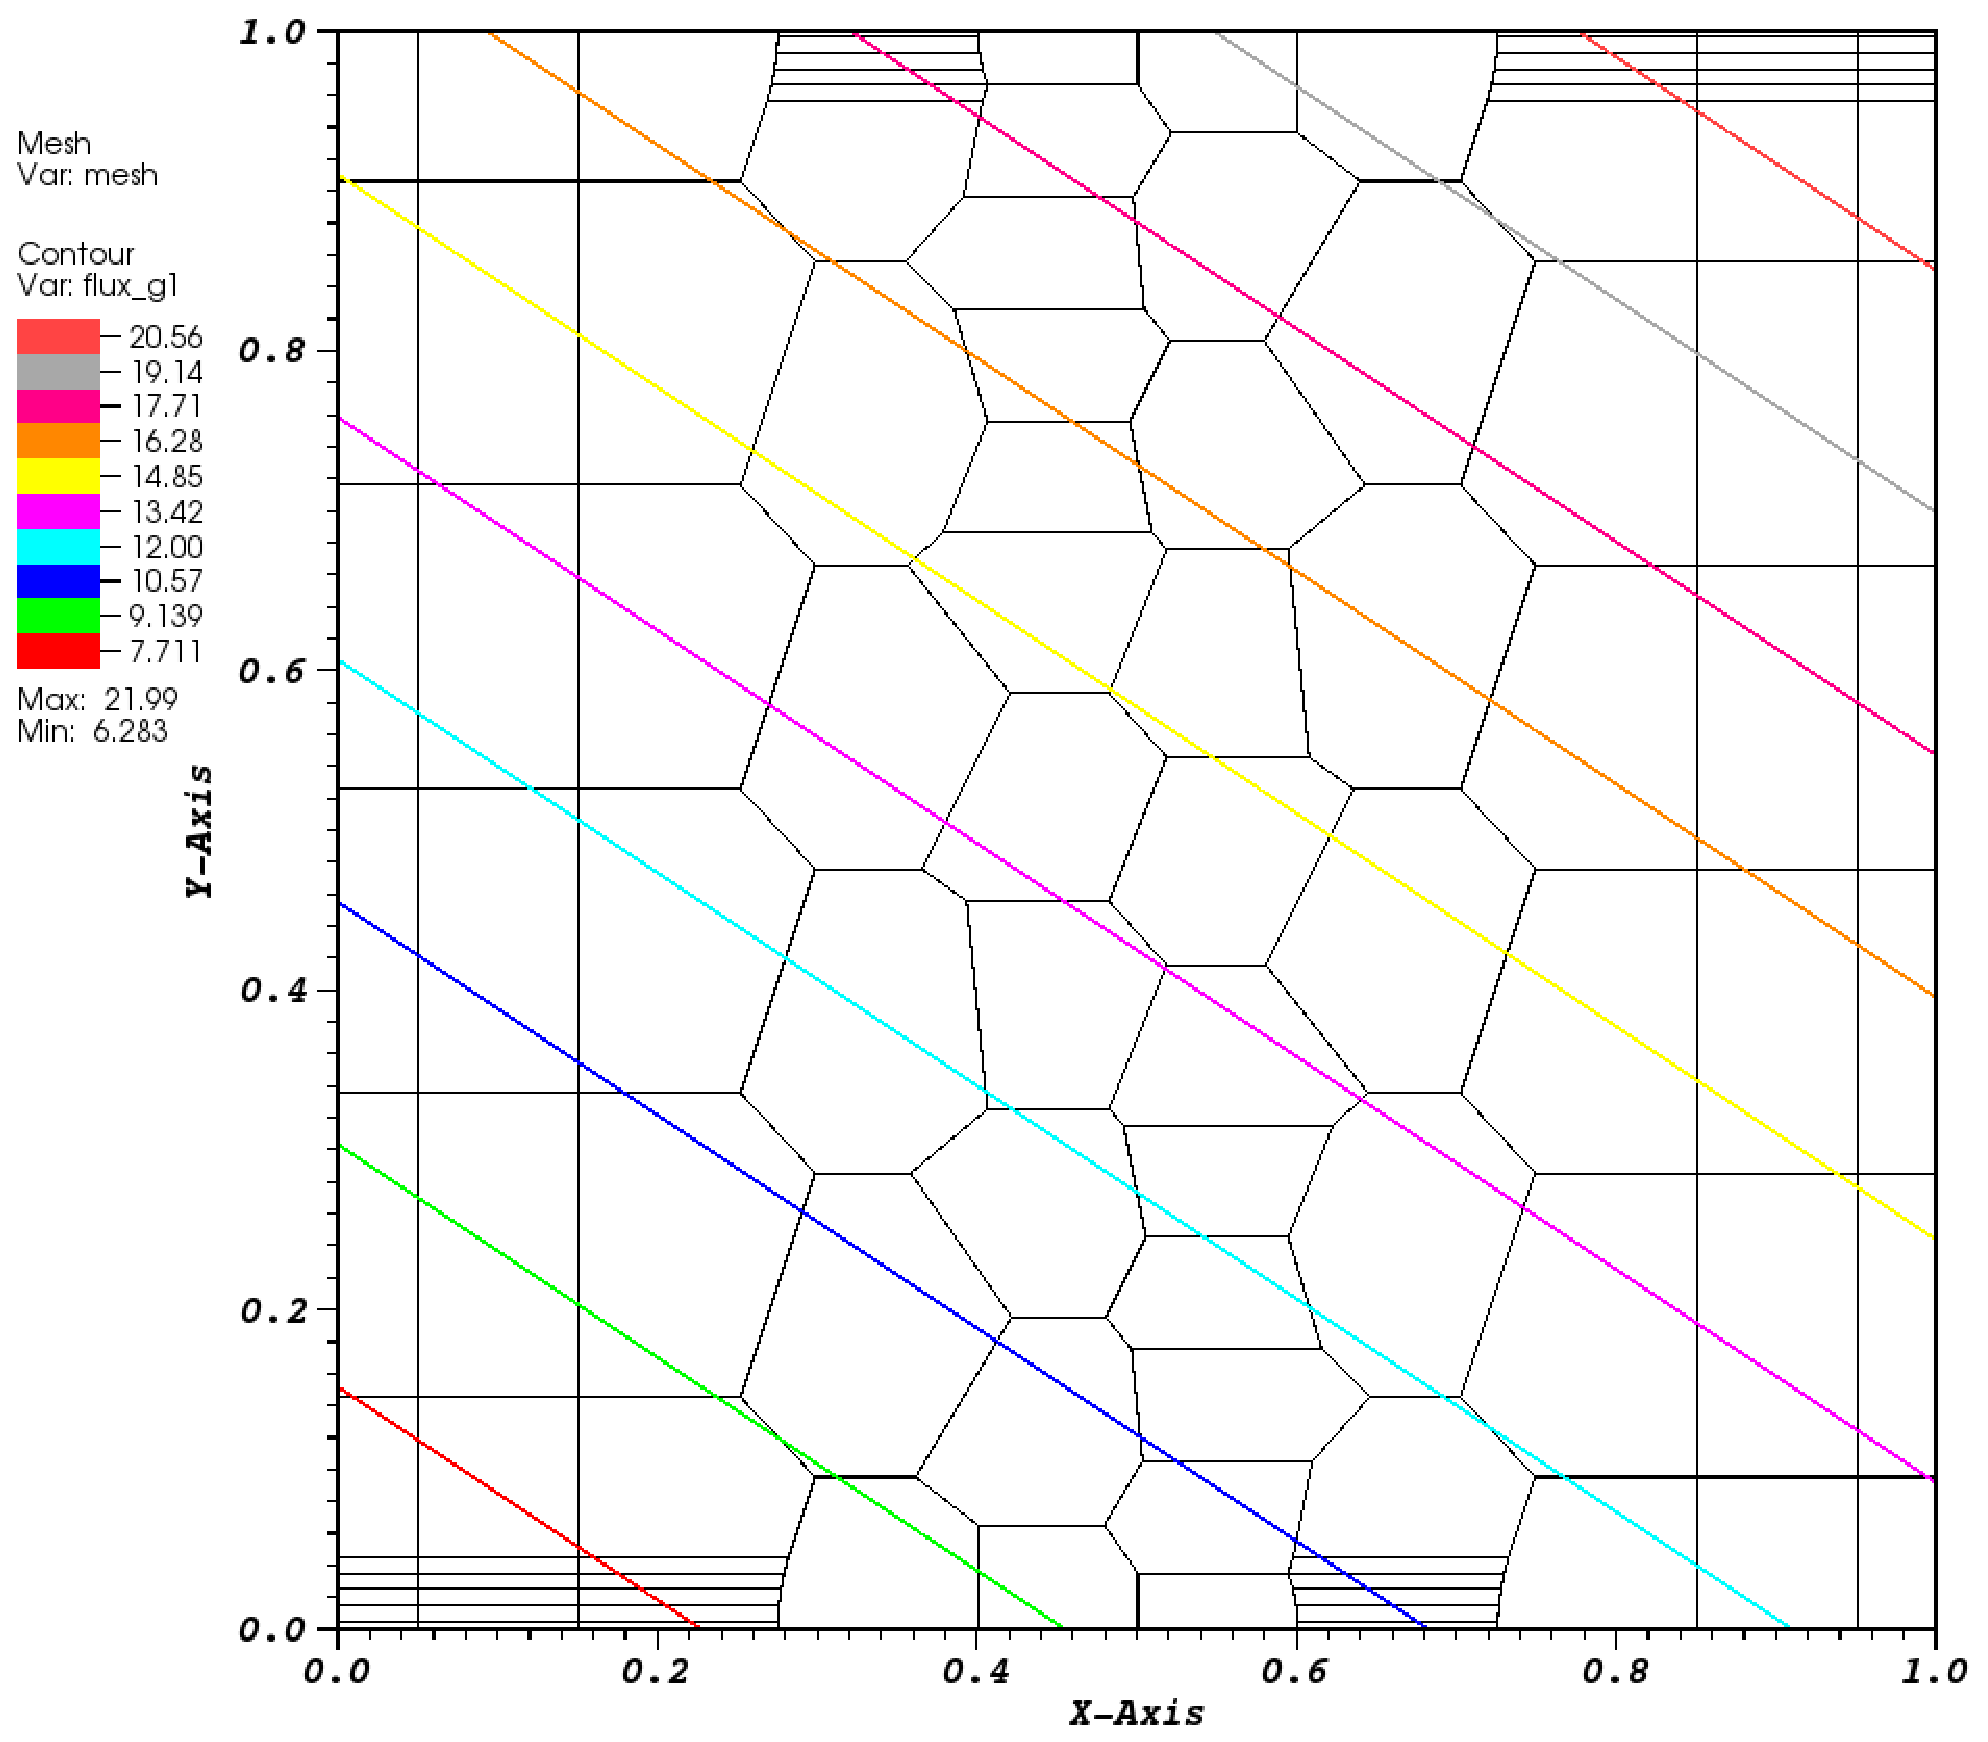
\includegraphics[width=\textwidth]{figures/sec_BF/z_poly_MAXENT_k1.eps}
		\caption{}
	\end{subfigure}
\caption{Contour plots of the exactly-linear solution with the linear maximum entropy basis functions on (a) cartesian mesh, (b) ordered-triangular mesh, (c) quadrilateral shestakov mesh, (d) sinusoidal polygonal mesh, (e) quadrilateral z-mesh, and (f) polygonal z-mesh.}
\label{fig::BF_Results_Linear_me1_sol}
\end{figure}

\begin{figure}
\centering
	\begin{subfigure}[b]{0.45\textwidth}
		\centering
		\label{subfig::cart_me_k2_lin_sol}
		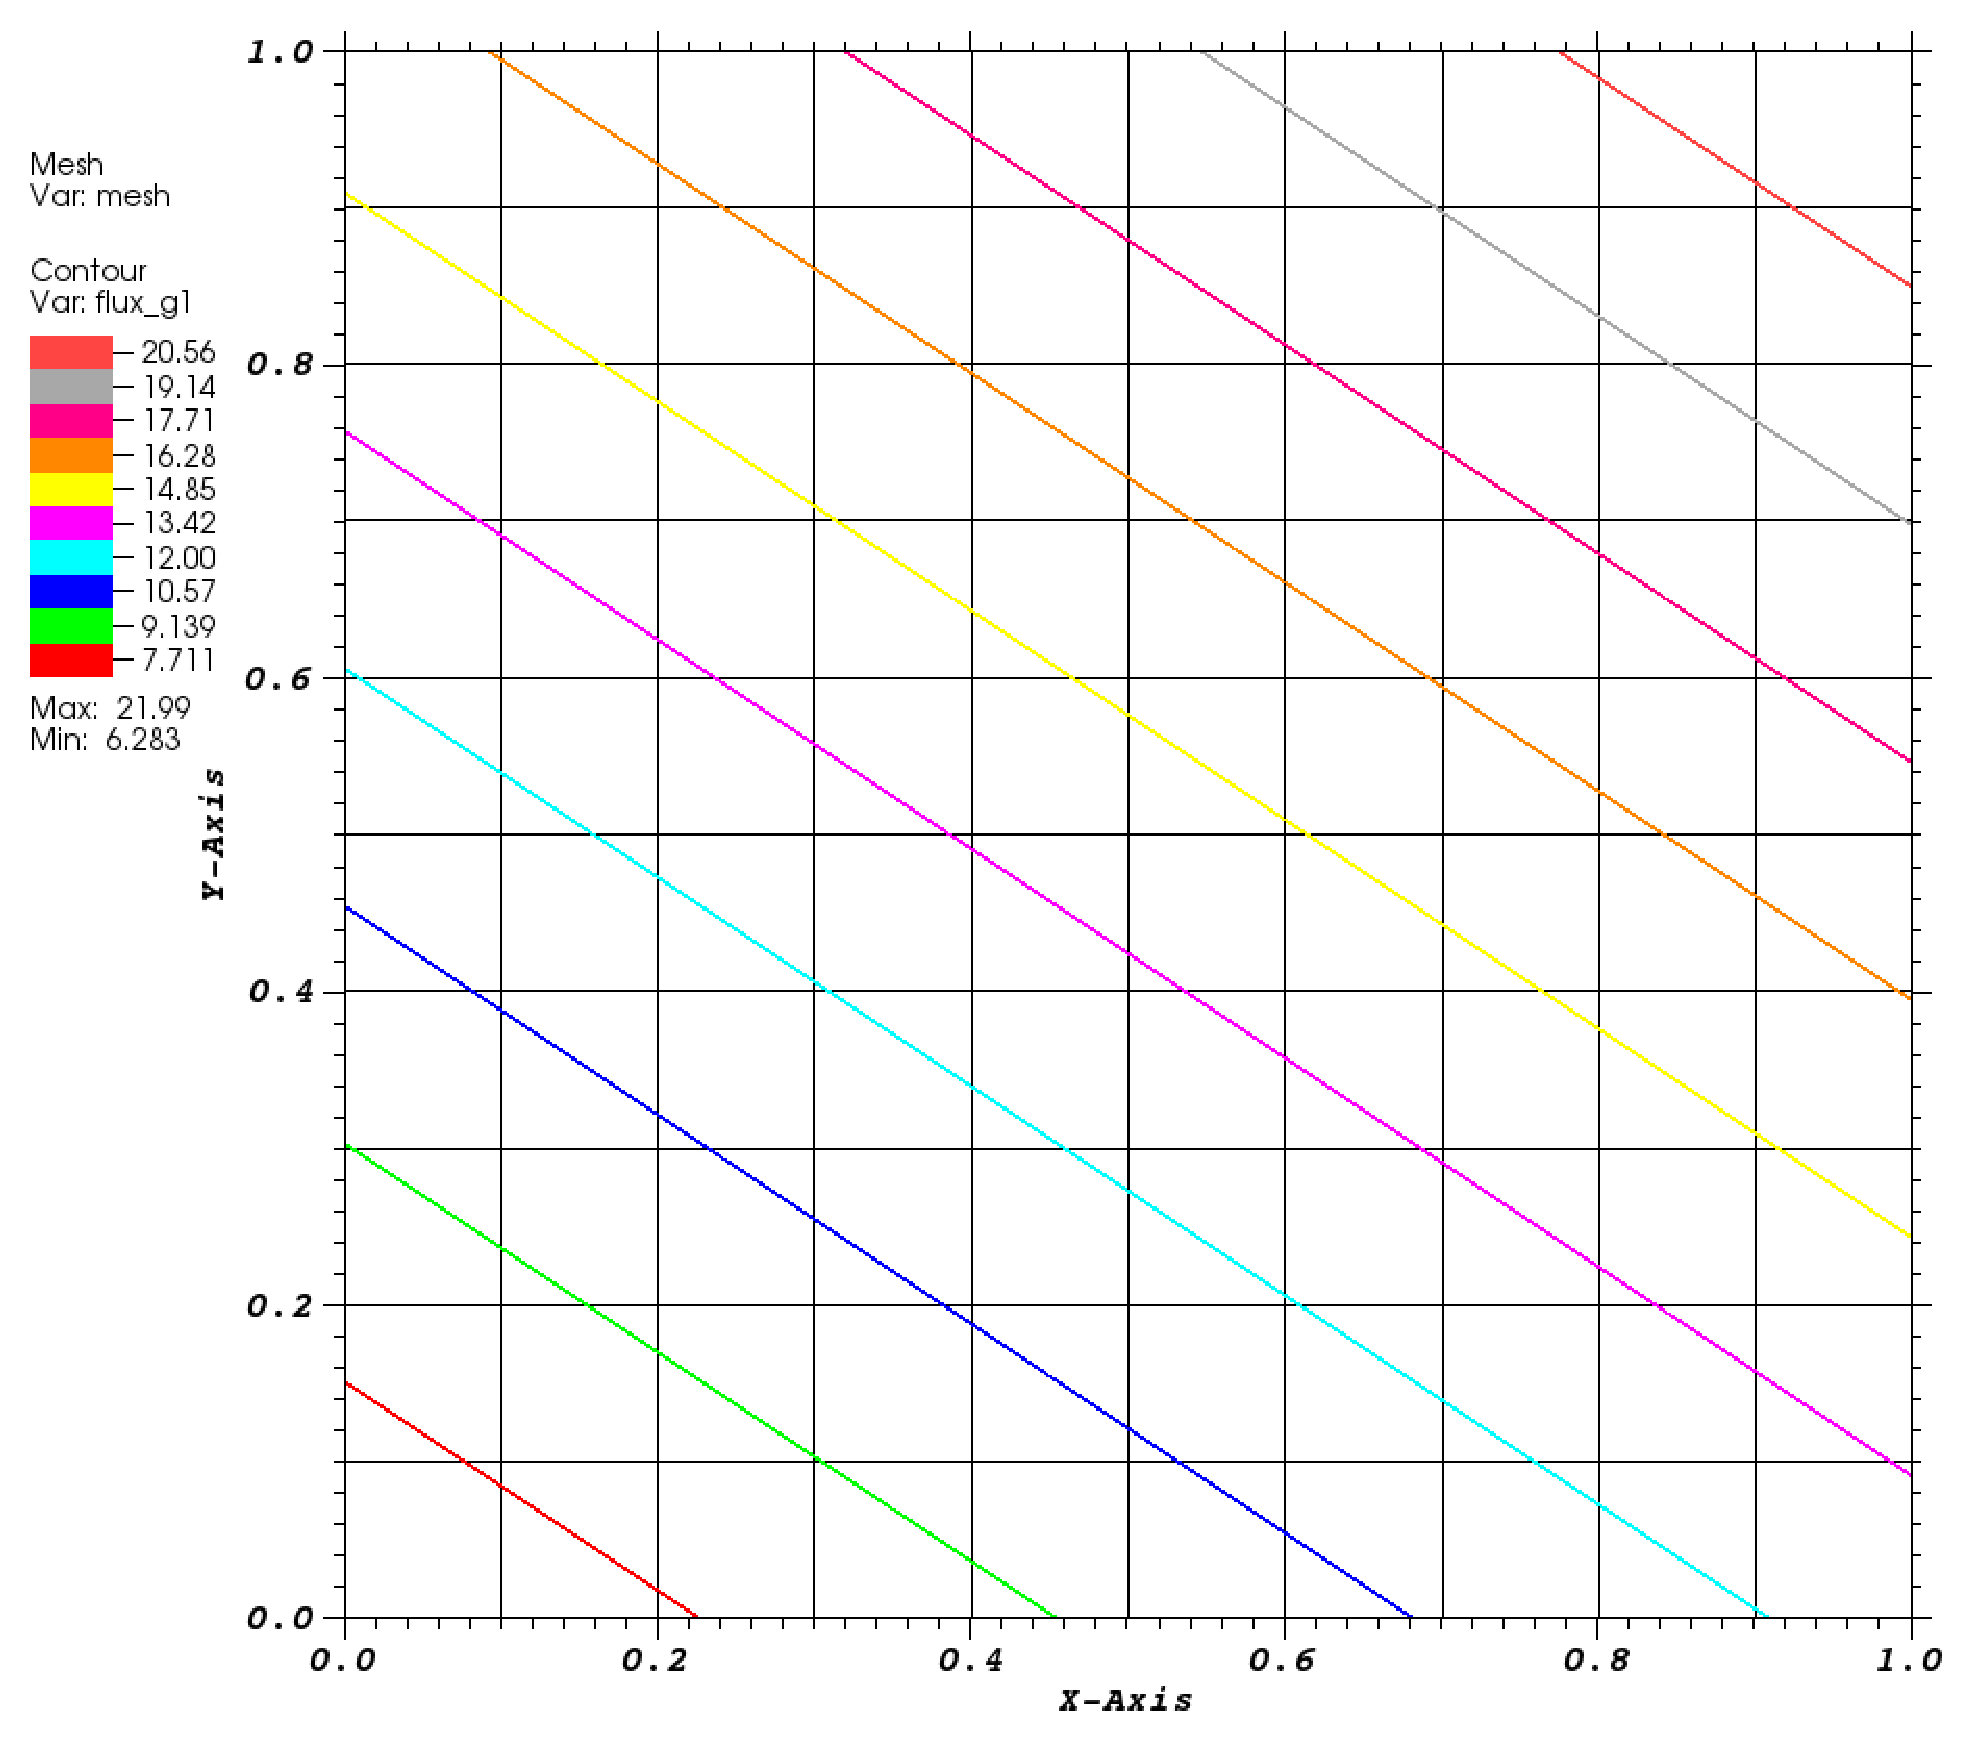
\includegraphics[width=\textwidth]{figures/sec_BF/cart_MAXENT_k2.eps}
		\caption{}
	\end{subfigure}
	\hfill
	\begin{subfigure}[b]{0.45\textwidth}
		\centering
		\label{subfig::tri_me_k2_lin_sol}
		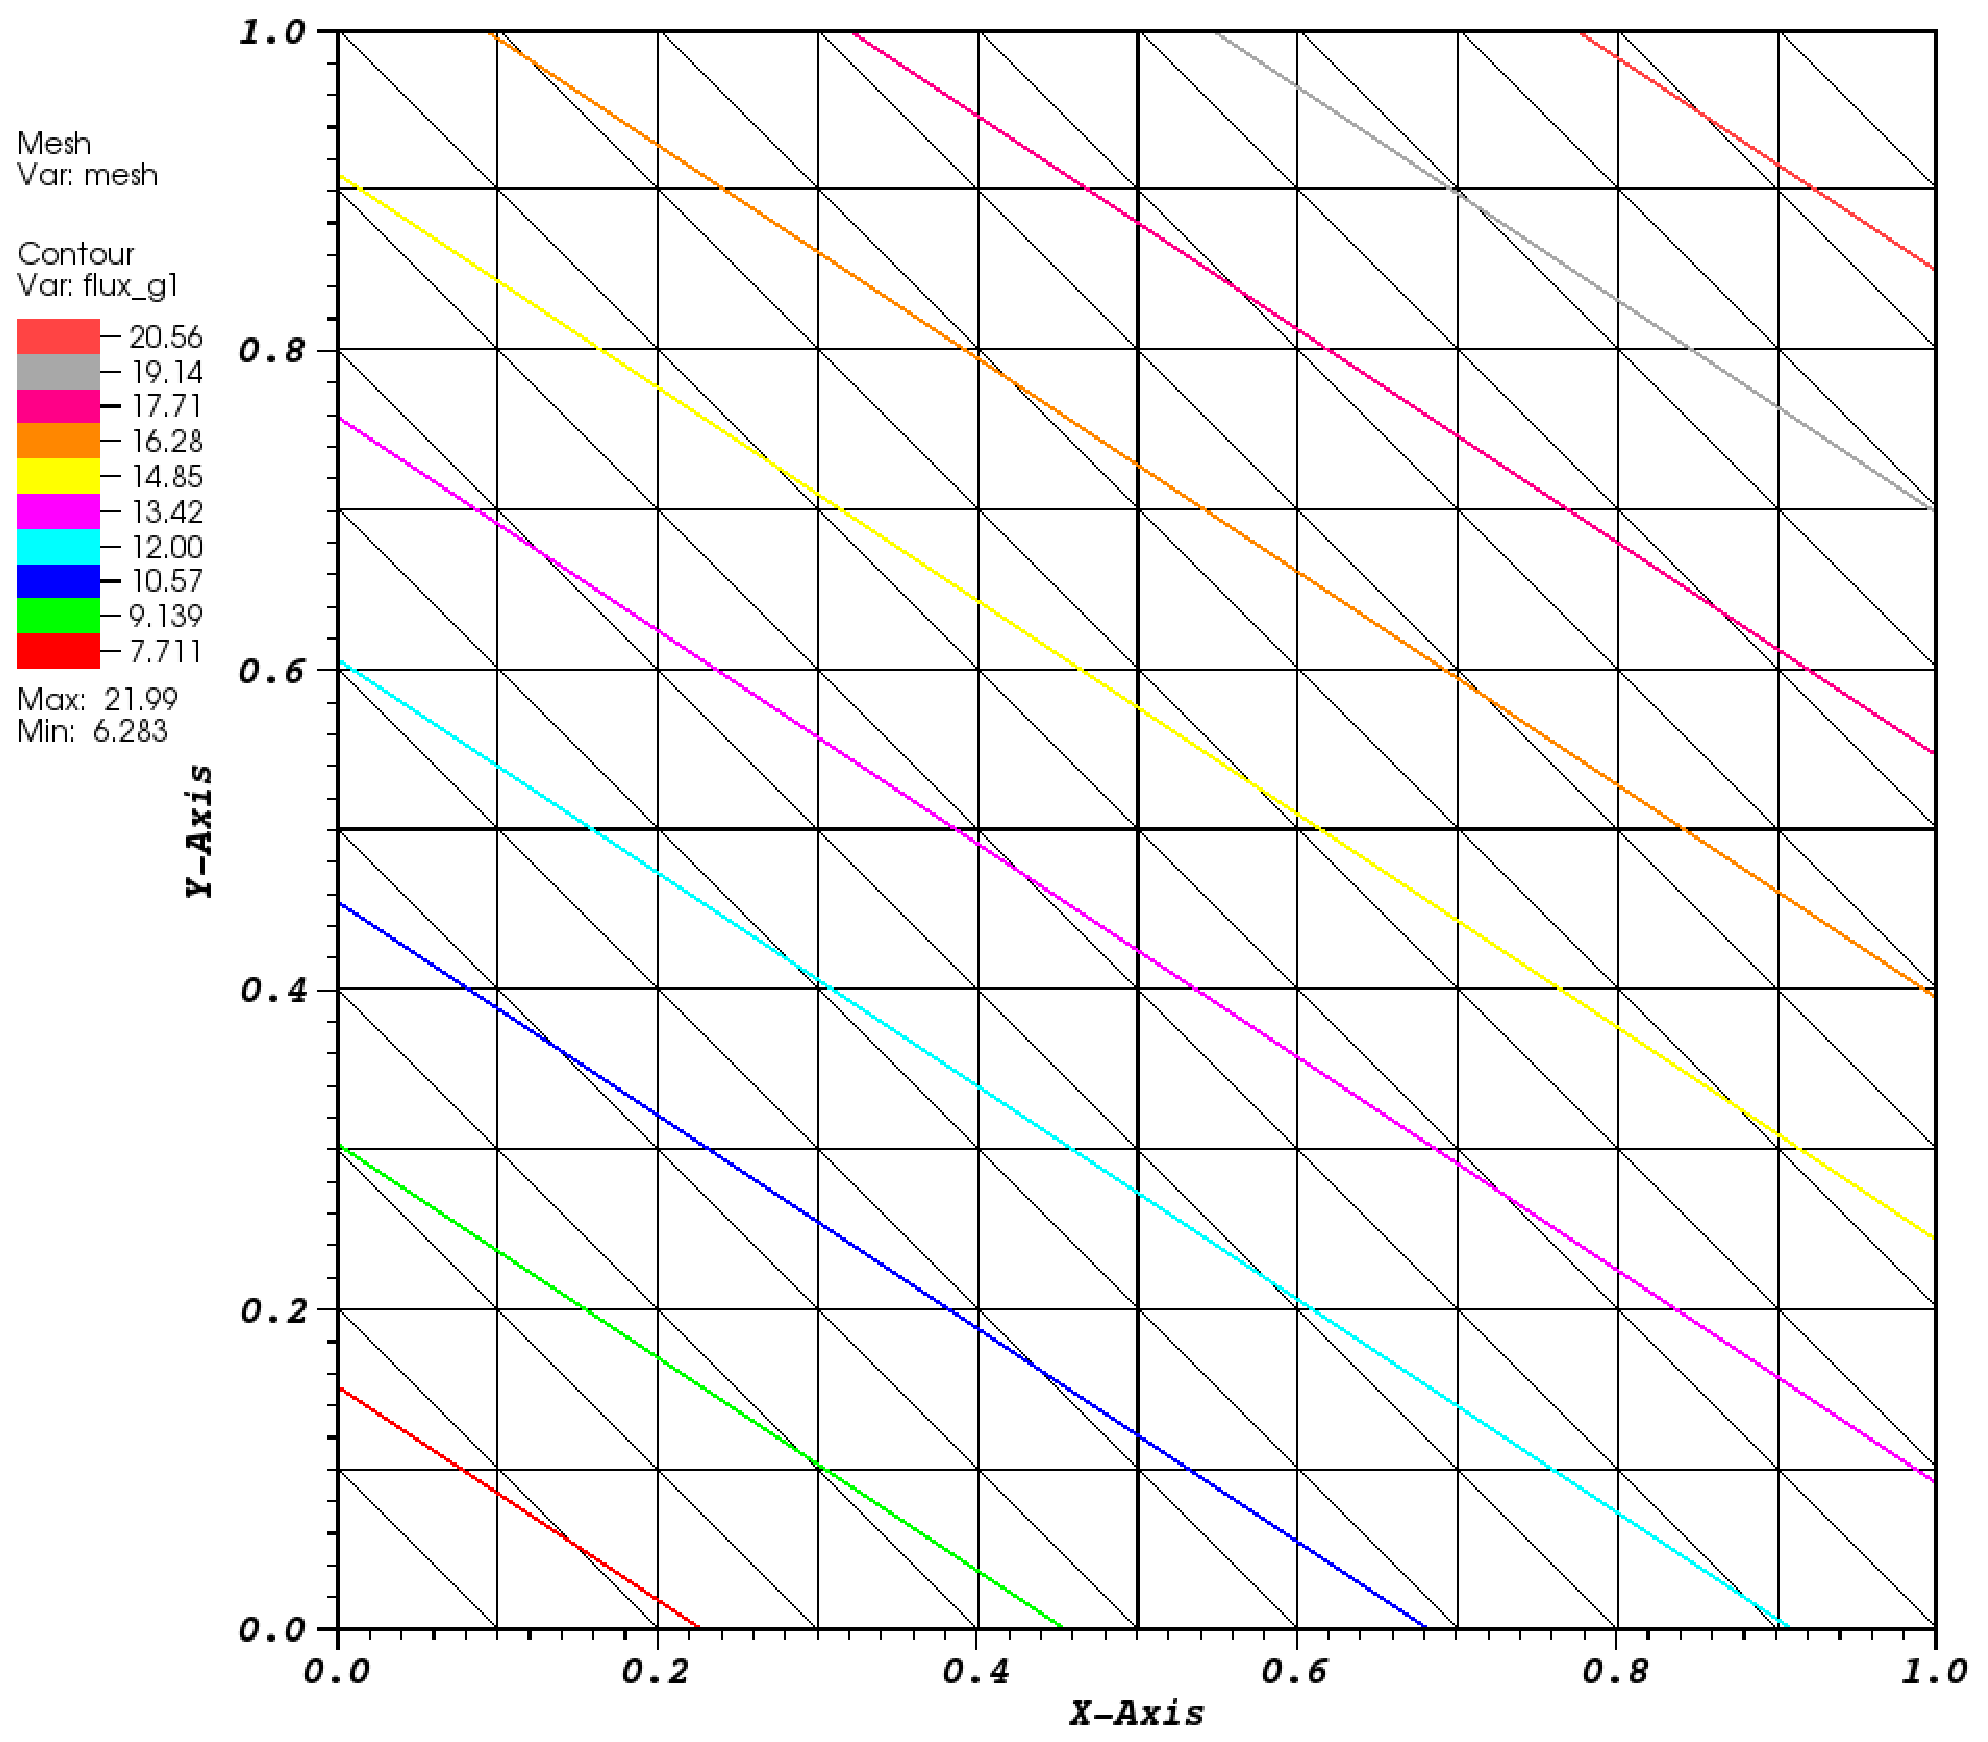
\includegraphics[width=\textwidth]{figures/sec_BF/tri_MAXENT_k2.eps}
		\caption{}
	\end{subfigure}
	\vfill
	\begin{subfigure}[b]{0.45\textwidth}
		\centering
		\label{subfig::shes_quad_me_k2_lin_sol}
		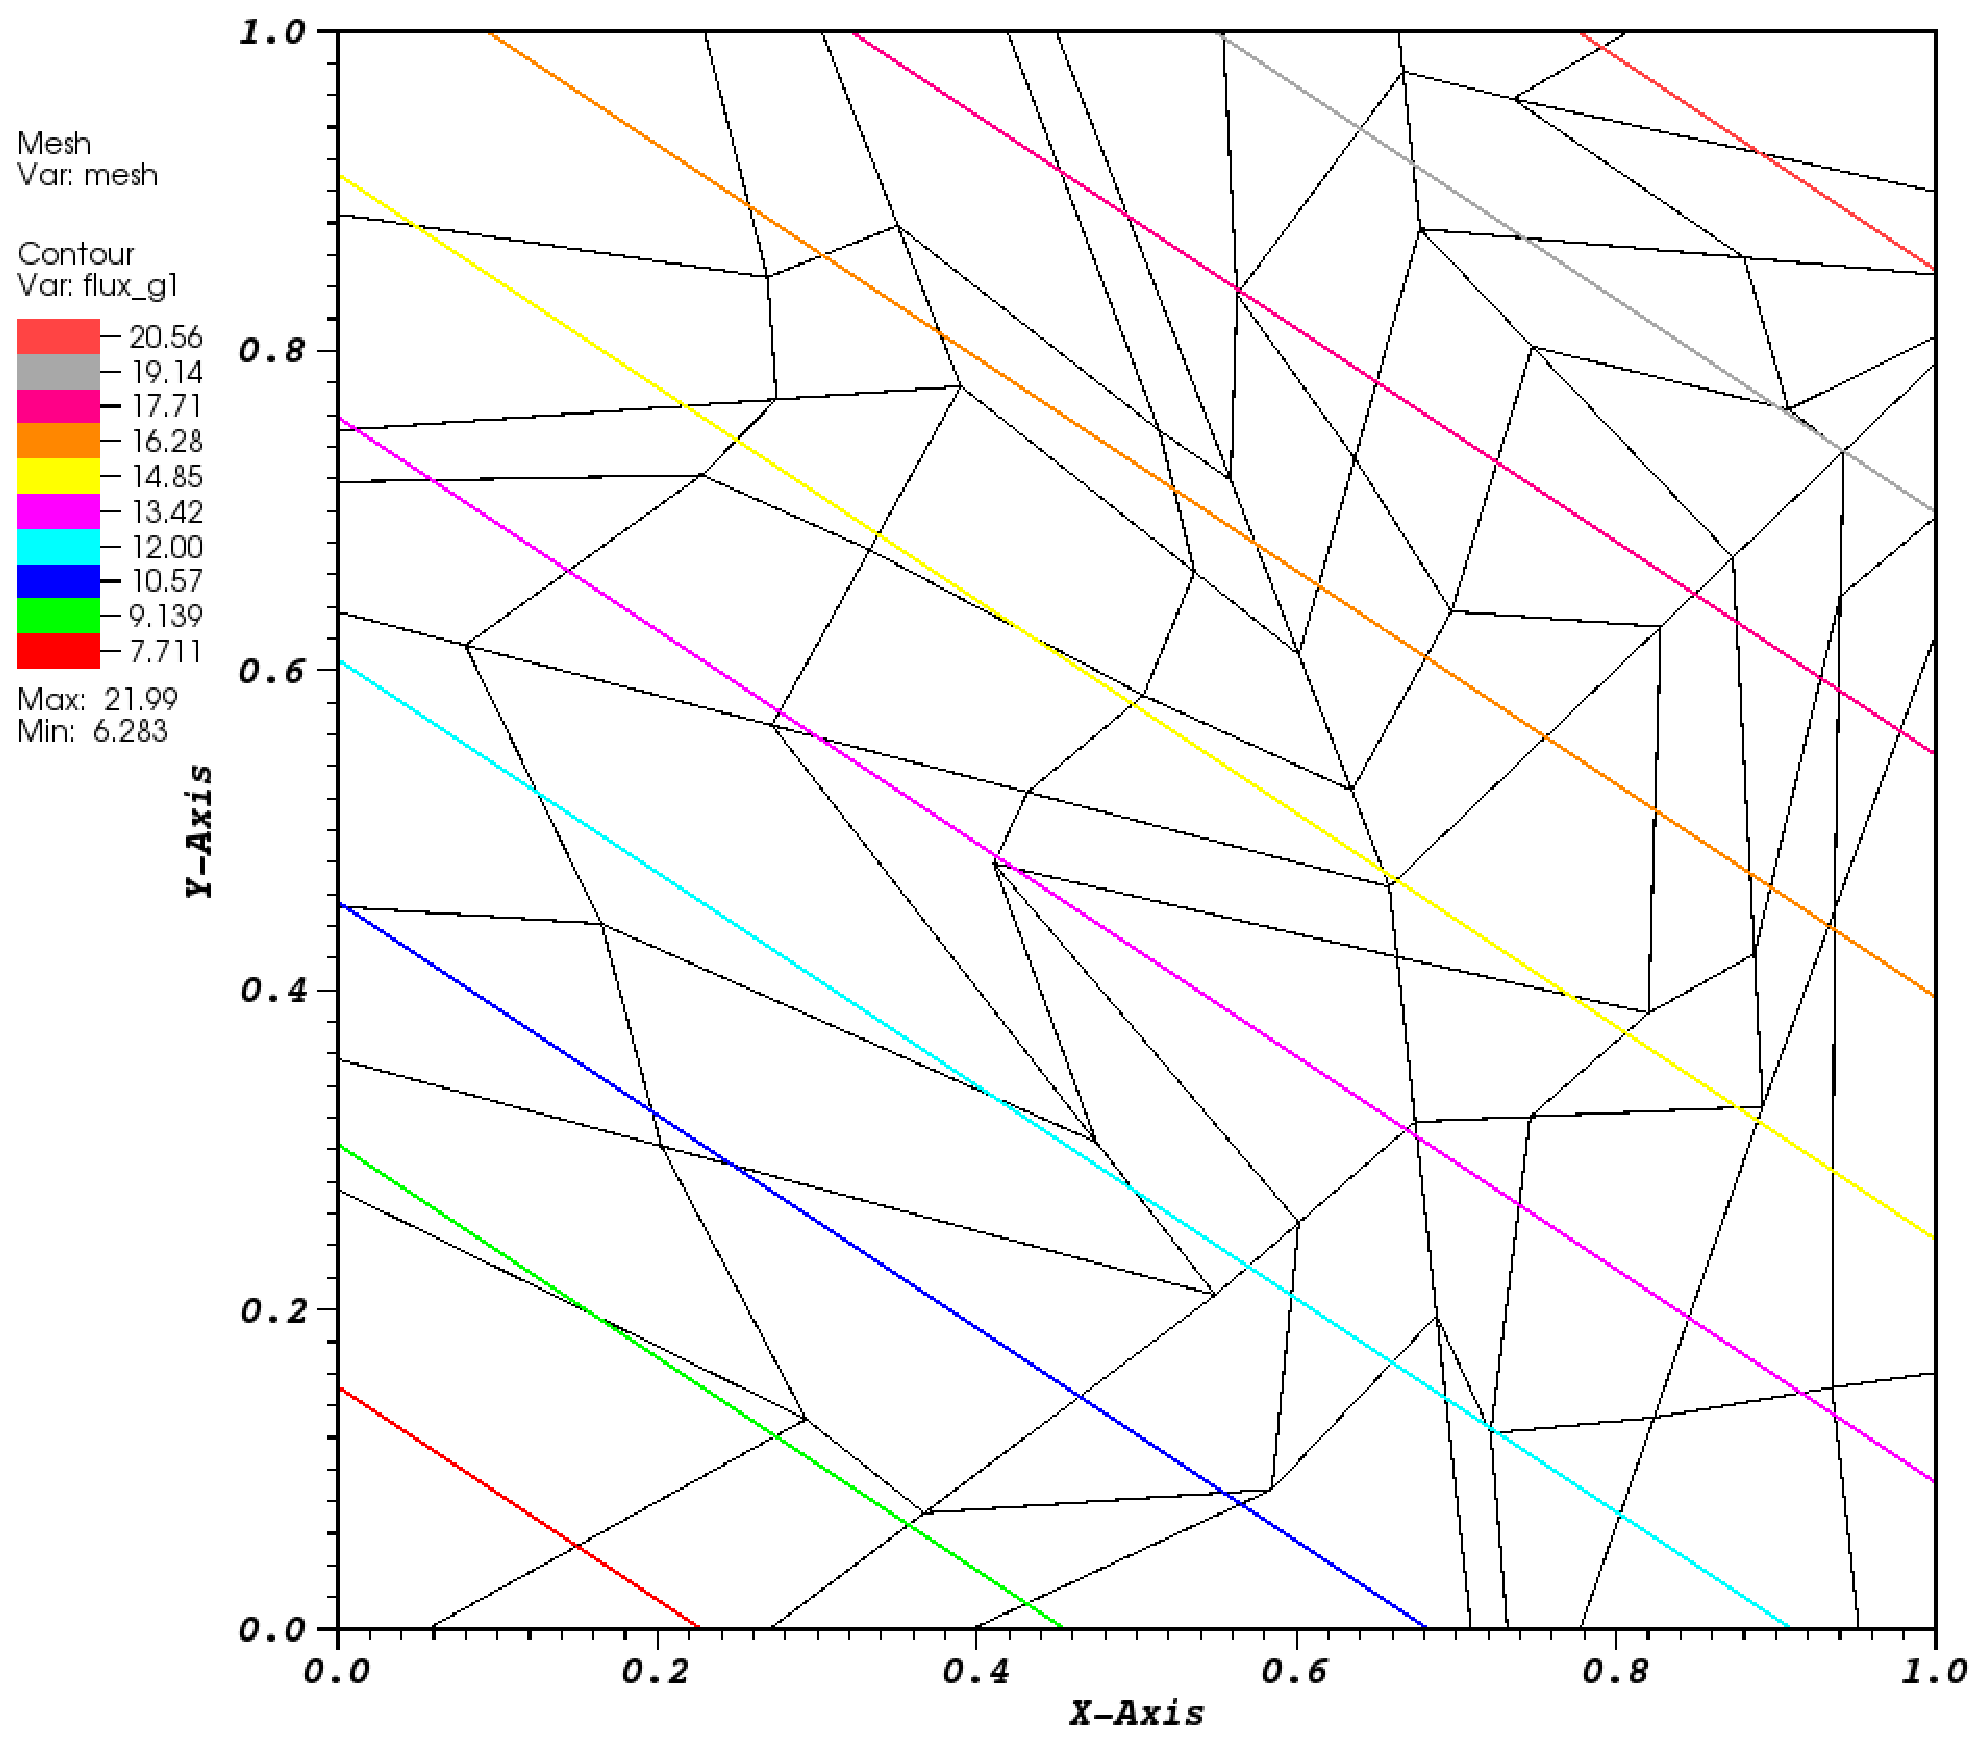
\includegraphics[width=\textwidth]{figures/sec_BF/shes_quad_MAXENT_k2.eps}
		\caption{}
	\end{subfigure}
	\hfill
	\begin{subfigure}[b]{0.45\textwidth}
		\centering
		\label{subfig::smooth_poly_me_k2_lin_sol}
		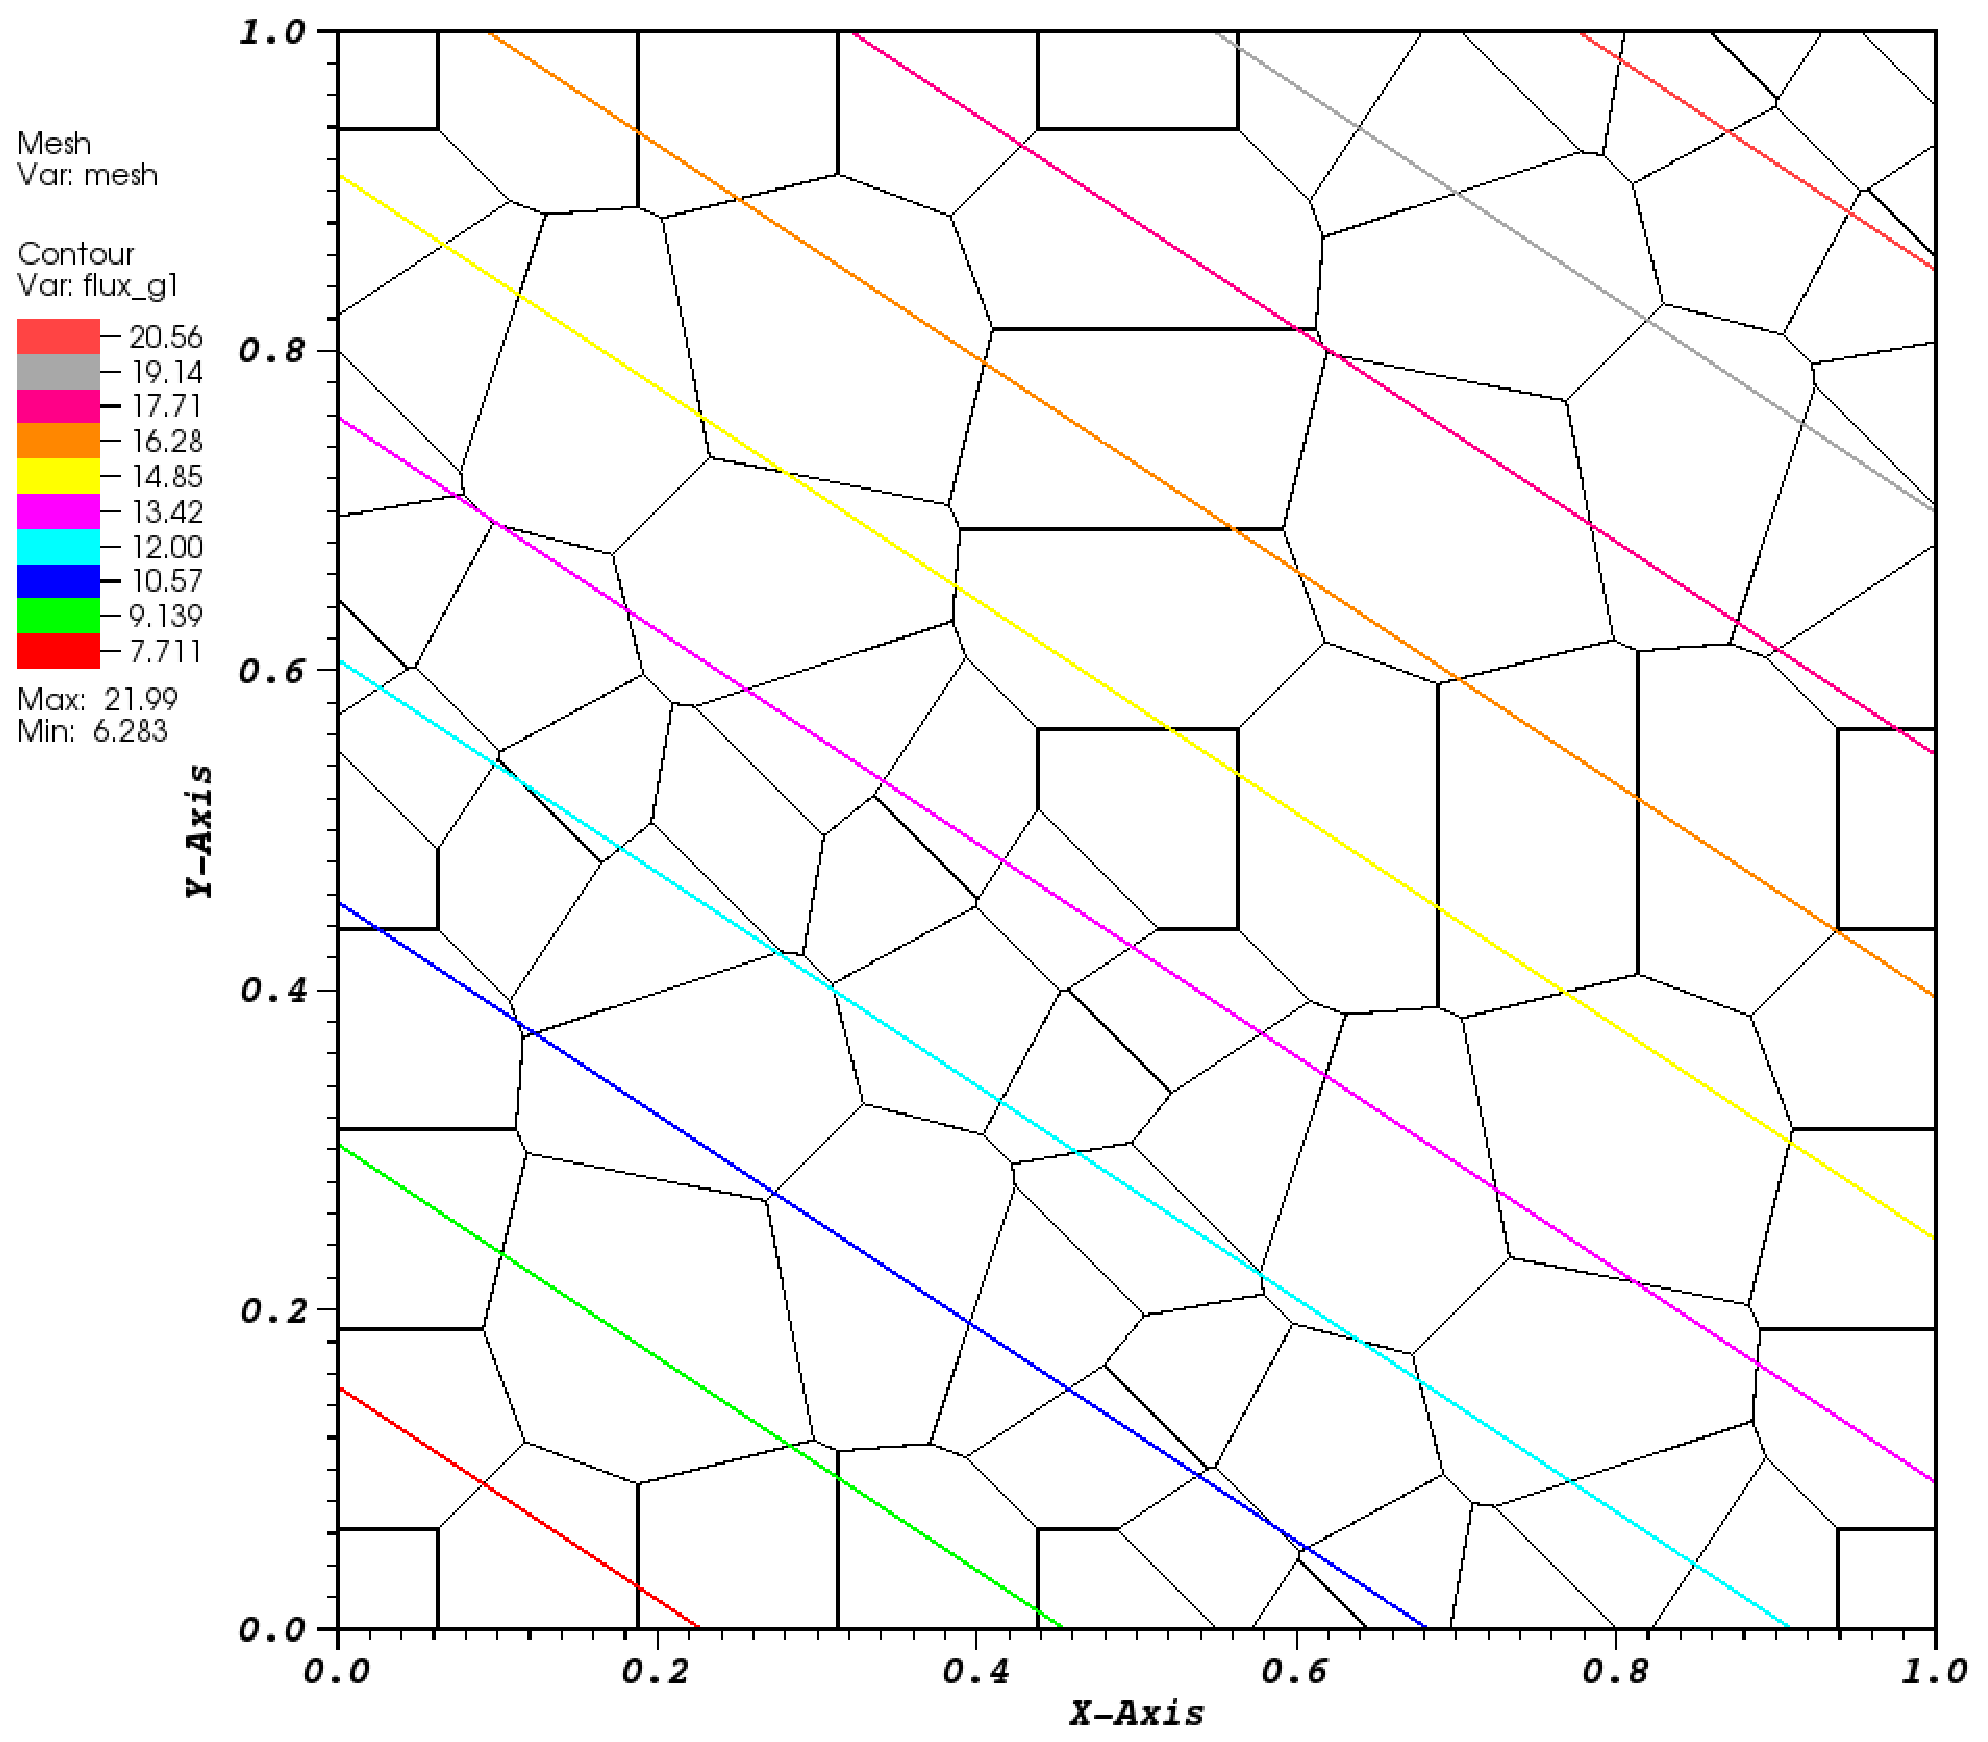
\includegraphics[width=\textwidth]{figures/sec_BF/smooth_poly_MAXENT_k2.eps}
		\caption{}
	\end{subfigure}
	\vfill
	\begin{subfigure}[b]{0.45\textwidth}
		\centering
		\label{subfig::z_quad_me_k2_lin_sol}
		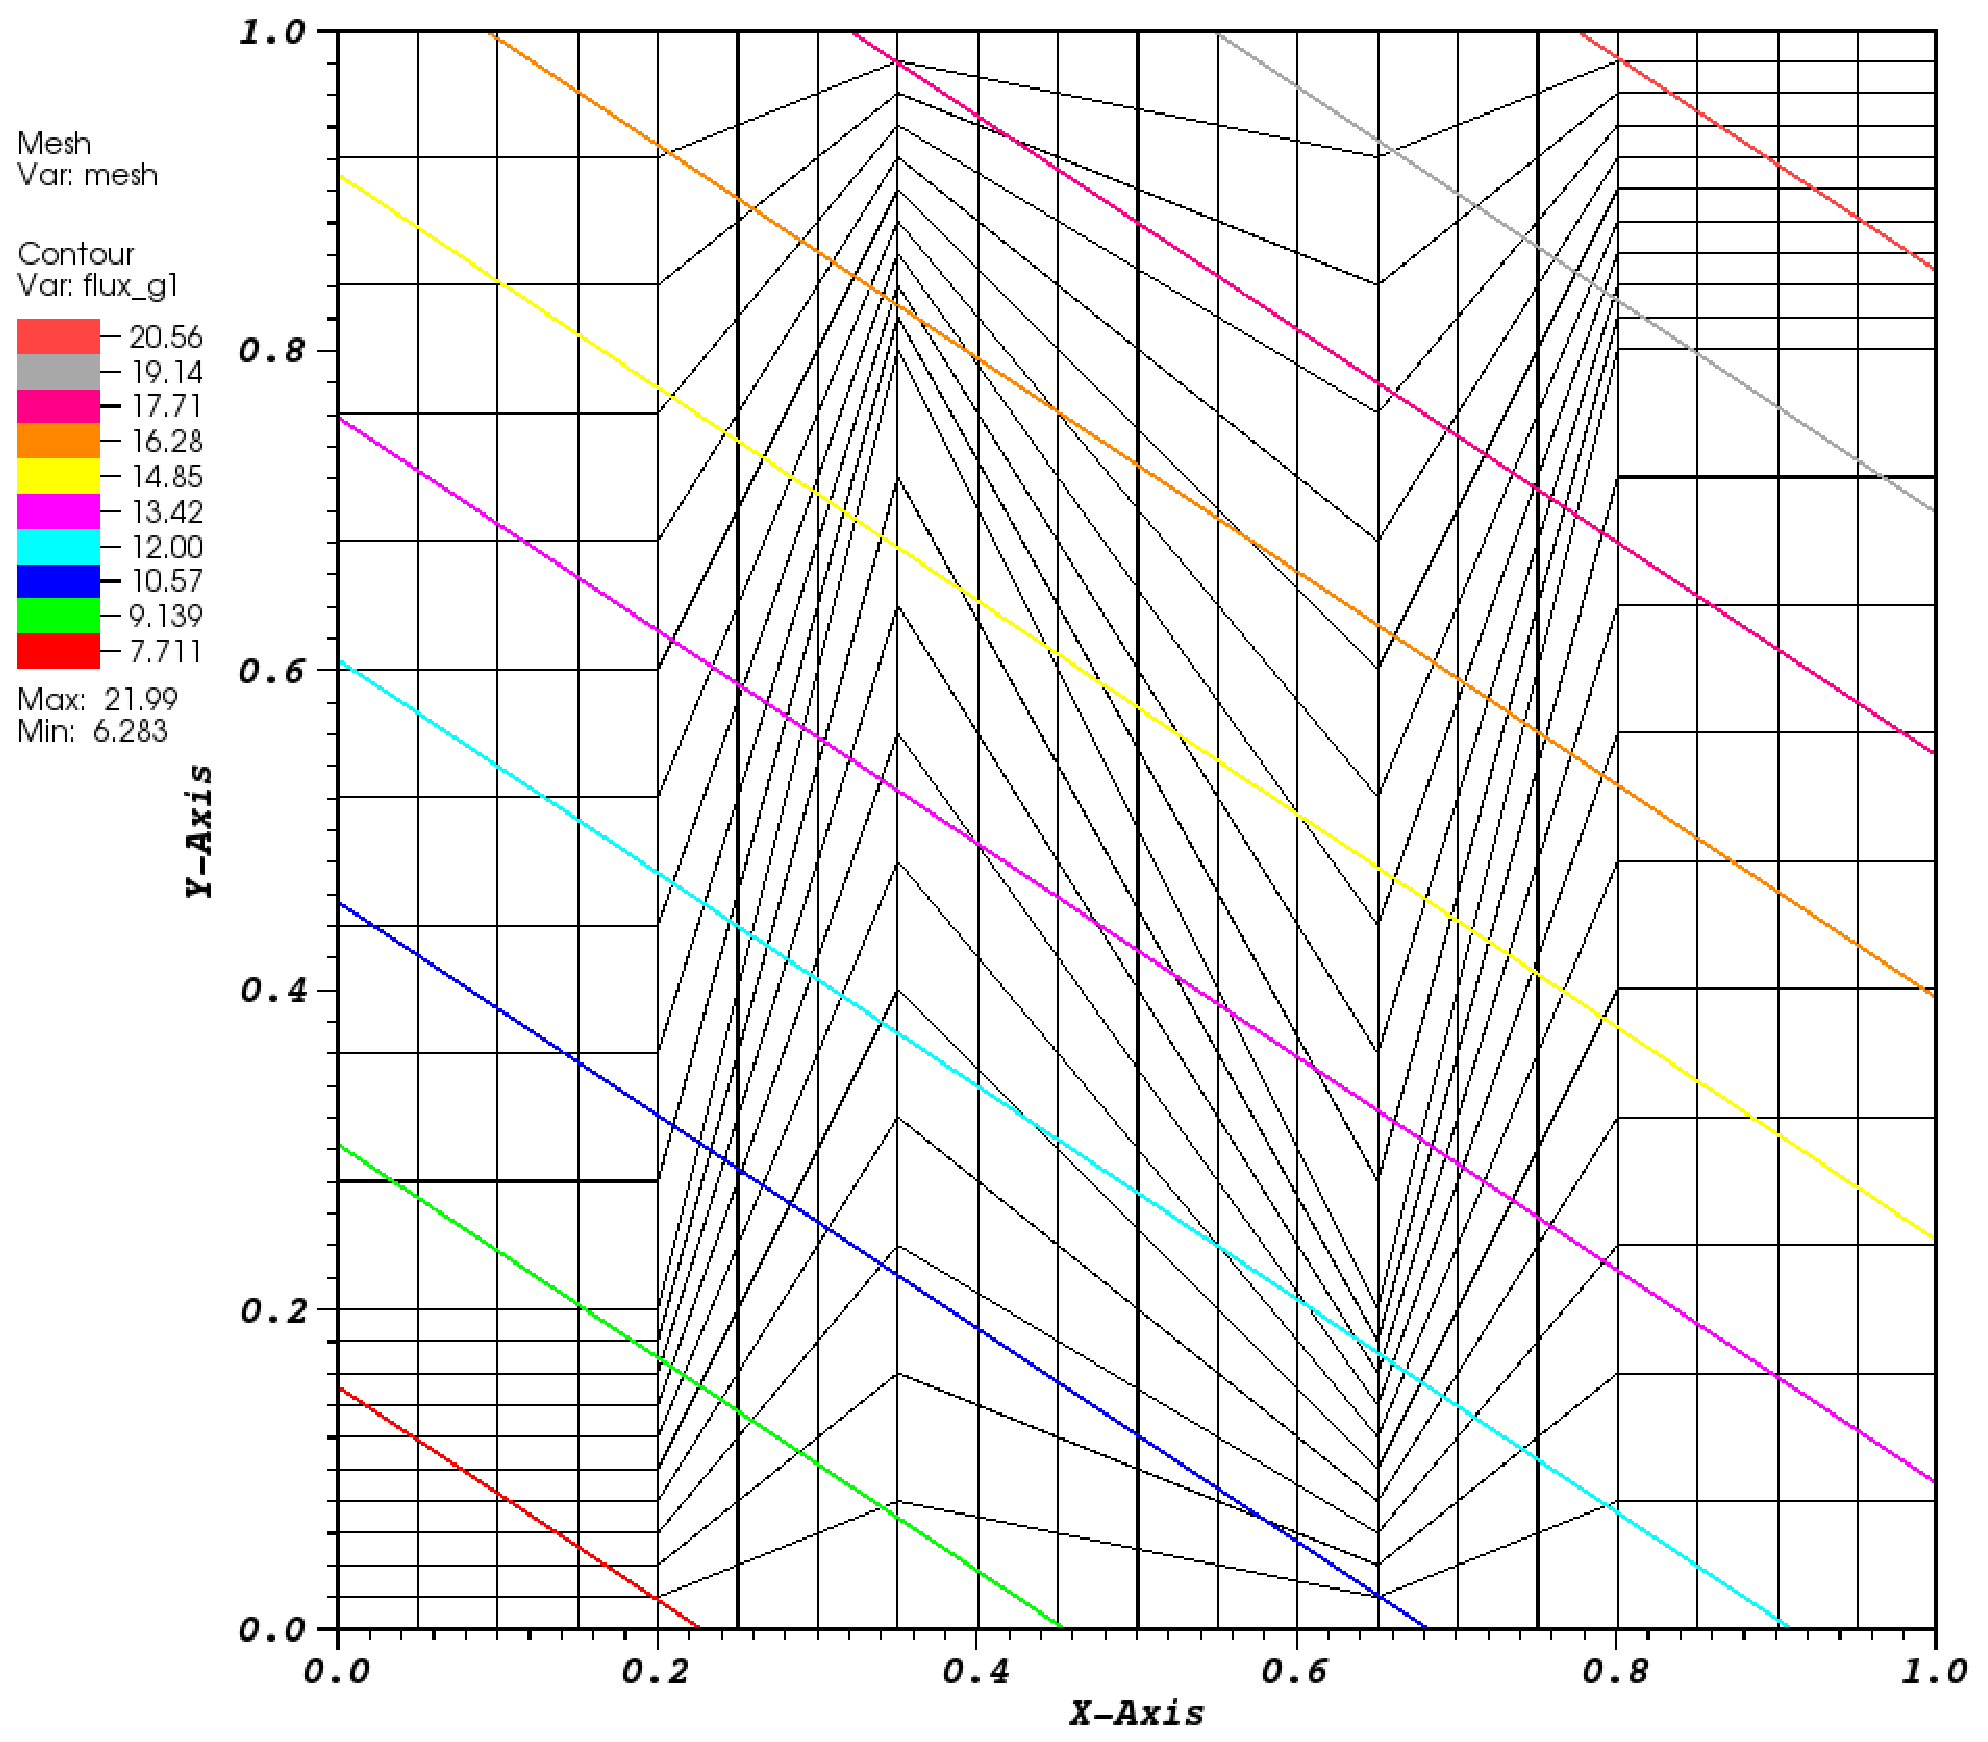
\includegraphics[width=\textwidth]{figures/sec_BF/z_quad_MAXENT_k2.eps}
		\caption{}
	\end{subfigure}
	\hfill
	\begin{subfigure}[b]{0.45\textwidth}
		\centering
		\label{subfig::z_poly_me_k2_lin_sol}
		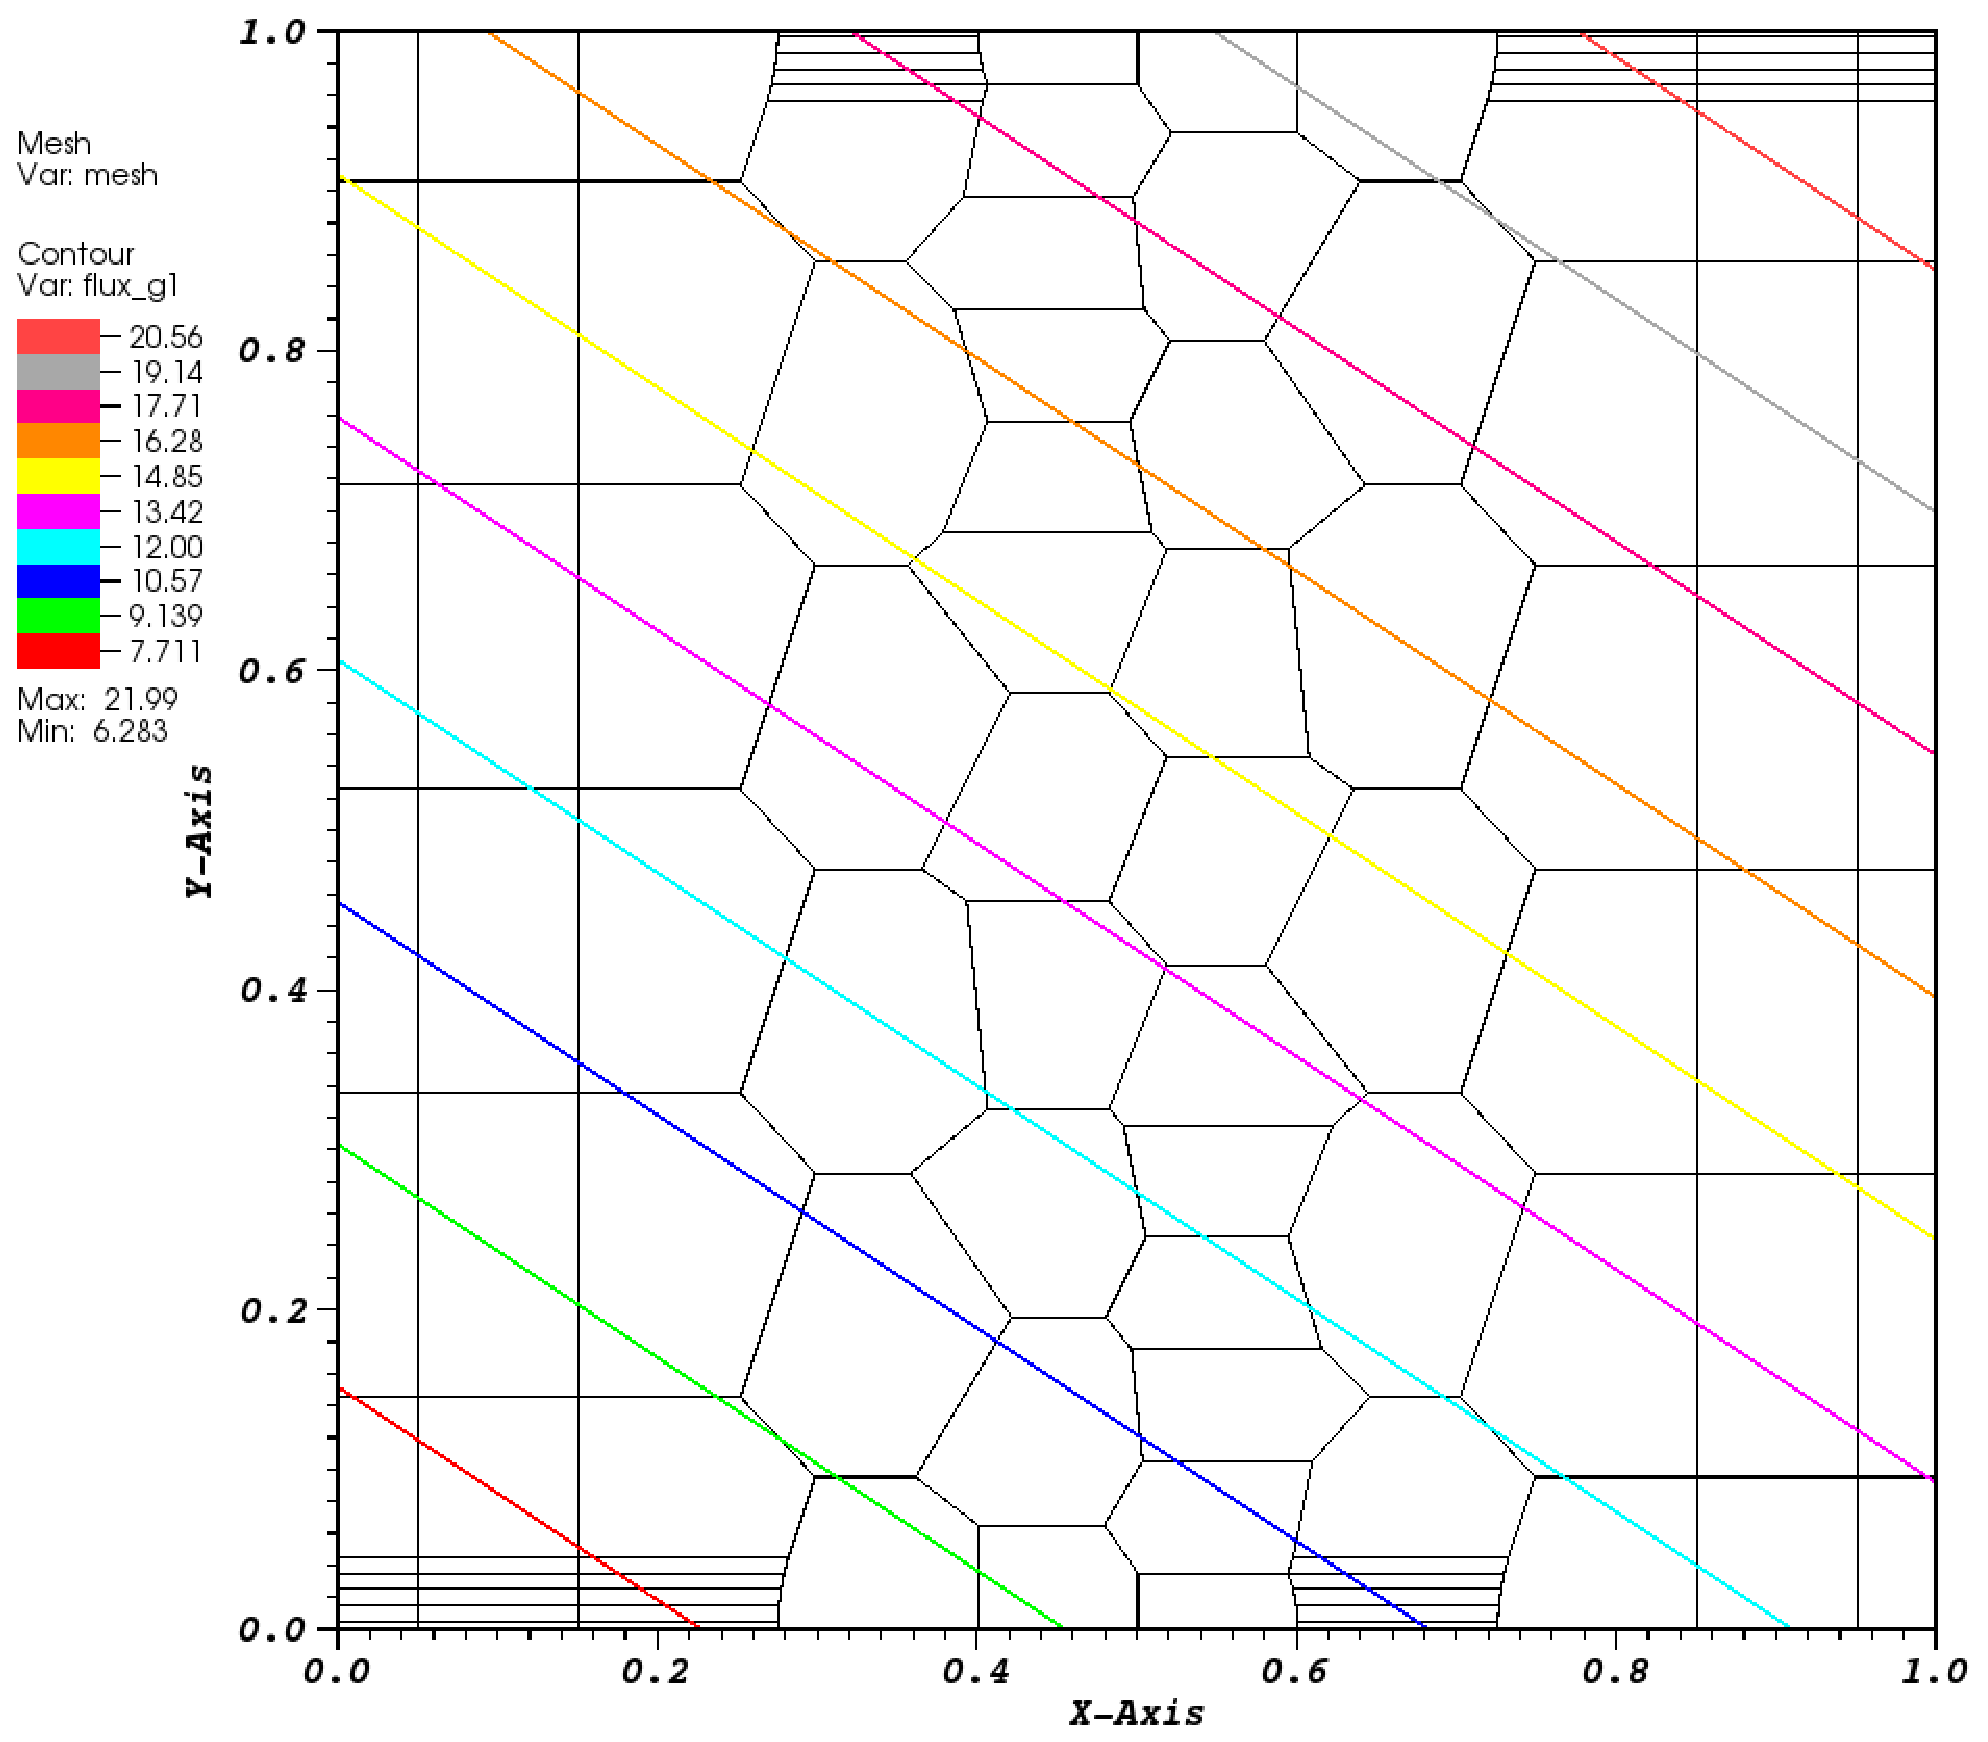
\includegraphics[width=\textwidth]{figures/sec_BF/z_poly_MAXENT_k2.eps}
		\caption{}
	\end{subfigure}
\caption{Contour plots of the exactly-linear solution with the quadratic serendipity maximum entropy basis functions on (a) cartesian mesh, (b) ordered-triangular mesh, (c) quadrilateral shestakov mesh, (d) sinusoidal polygonal mesh, (e) quadrilateral z-mesh, and (f) polygonal z-mesh.}
\label{fig::BF_Results_Linear_me2_sol}
\end{figure}

%%%%%%%%%%%%%%%%%%%%%%%%%%%%%%%%%%%%%%%%%%%%%%%%%%%
%%%   SubSection - MMS
\subsection{Convergence Rate Analysis by the Method of Manufactured Solutions}
\label{sec::BF_Results_MMS}

The next numerical example we investigate involves calculating the convergence rate of the solution error via the method of manufactured solutions (MMS). Like MES, MMS enforces a given solution by use of a derived functional form for the driving source of the problem ($Q_{ext}$). However, unlike MES, we enforce a spatial solution that cannot be captured by the interpolation of the finite element space. Using a specification of the Bramble-Hilbert \cite{bramble1970estimation} lemma, the difference between the exact solution, $\Phi_e$, and the discretized solution, $\Phi_h$, residing in the Sobolev space, $W_{\mathcal{D}}^h \in \mathcal{T}_h$, for a given polynomial interpolation order, $k$, is

\begin{equation}
\label{eq::BF_Results_MMS_errnorm}
|| \Phi_{e} - \Phi_h || _{2}  \leq C \frac{h^{q+1/2}}{(k+1)^q} ,
\end{equation}

\noindent where $q=\min(k+1/2,r )$, $h$ is the maximum diameter of all mesh cells, $C$ is some constant independent of the mesh, $r$ is a measure of the regularity of the transport solution, and $|| \cdot ||_2$ is the $L_2$ norm \cite{houston2000stabilized}. For transport solutions with sufficient discontinuities, $r$ can approach 0. However, if the chosen solution is at least $C^k$ continuous and a topologically regular mesh is used, then the convergence rate becomes strictly $(k+1)$. For structured meshes, $h$ is straightforward to define. Unfortunately, this becomes a problem in general for polytope meshes. Instead, the grid resolution can be related to the number of spatial degrees of freedom ($N_{dof}$),

\begin{equation}
\label{eq::BF_Results_MMS_dofres}
N_{dof} \propto h^{-d} ,
\end{equation}

\noindent where $d$ is the dimensionality of the problem. Using this relationship for the grid resolution, along with the error norm of Eq. (\ref{eq::BF_Results_MMS_errnorm}), we can define a general relationship between the error norm and the number of spatial degrees of freedom:

\begin{equation}
\label{eq::BF_Results_MMS_errdofres}
|| \Phi_{e} - \Phi_h || _{2}  \propto N_{dof}^{- \frac{k+1}{d}} .
\end{equation}

\noindent The result of Eq. (\ref{eq::BF_Results_MMS_errdofres}) states that we expect convergence rates of $N_{dof}^{-1}$ and $N_{dof}^{-2/3}$ for linear basis functions in 2D and 3D, respectively. Conversely, quadratic basis functions will yield convergence rates of $N_{dof}^{-3/2}$ and $N_{dof}^{-1}$ in 2D and 3D, respectively.

For this example, we choose the following solution and problem parameters and characteristics:

\begin{enumerate}
	\item Constant total cross section so that parameterized material properties are not necessary;
	\item No scattering to avoid solution discontinuities from the $S_N$ discretization;
	\item Analytical solutions that are $C^{\infty}$ continuous in space for both the angular flux and 0th order flux moment - this leads to valid solution spaces no matter what polynomial order is selected for the basis functions;
	\item The angular flux solution is zero on the boundary for all incident directions - this is identical to vacuum boundaries which can ease code development;
\end{enumerate}

\begin{equation}
\label{eq::BF_Results_MMS_fluxsols}
\begin{aligned}
\Psi (x,y) &= C_M x (L_x - x) y (L_y - y) \exp(-\frac{(x-x_0)^2 + (y-y_0)^2}{\gamma}) \\ 
\Phi (x,y) &= 2 \pi C_M x (L_x - x) y (L_y - y) \exp(-\frac{(x-x_0)^2 + (y-y_0)^2}{\gamma})
\end{aligned} .
\end{equation}

\noindent where the constants in the equations are:

\begin{equation}
\label{eq::BF_Results_MMS_consts}
C_M = \frac{200}{L_x^2 L_y^2} \qquad \gamma = \frac{L_x L_y}{100} .
\end{equation}

%%%%%%%%%%%%%%%%%%%%%%%%%%%%%%%%%%%%%%%%%%%%%%%%%%%
%%%   SubSection - Searchlight Problem
\subsection{Searchlight Problem}
\label{sec::BF_Results_SL}

The next example models a beam or searchlight. Similar problems were investigated in Dedner and Vollm{\"o}ller \cite{dedner2002adaptive} and Wang and Ragusa \cite{wang2011standard}. In this problem, an incident beam of neutrons is shined onto a small portion of a boundary, propagates through a vacuum, and then exits through a small portion of a different boundary. As the beam propagates through the vacuum, the spatial discretization causes radiation outflow through all downwind cell faces. This leads to numerical dispersion and will cause to beam to artificially broaden.

In this problem, we investigate an $\mathbb{R}^2$ domain of size $[0,1]^2$ cm. The radiation enters the left boundary between $0.2 \leq y \leq 0.4$ with an un-normalized angular direction of $[1,0.4]$. For this chosen direction, the radiation beam would analytically leave the right boundary between $0.6 \leq y \leq 0.8$. This means that any radiation leaving the right boundary for all other $y$ values is due to the numerical dispersion of the beam.

We investigated this problem using several of the 2D polygonal basis functions as outlined in Sections \ref{sec::BF_2DLinear} and \ref{sec::BF_2DQuadratic} as well as 

\begin{figure}
\centering
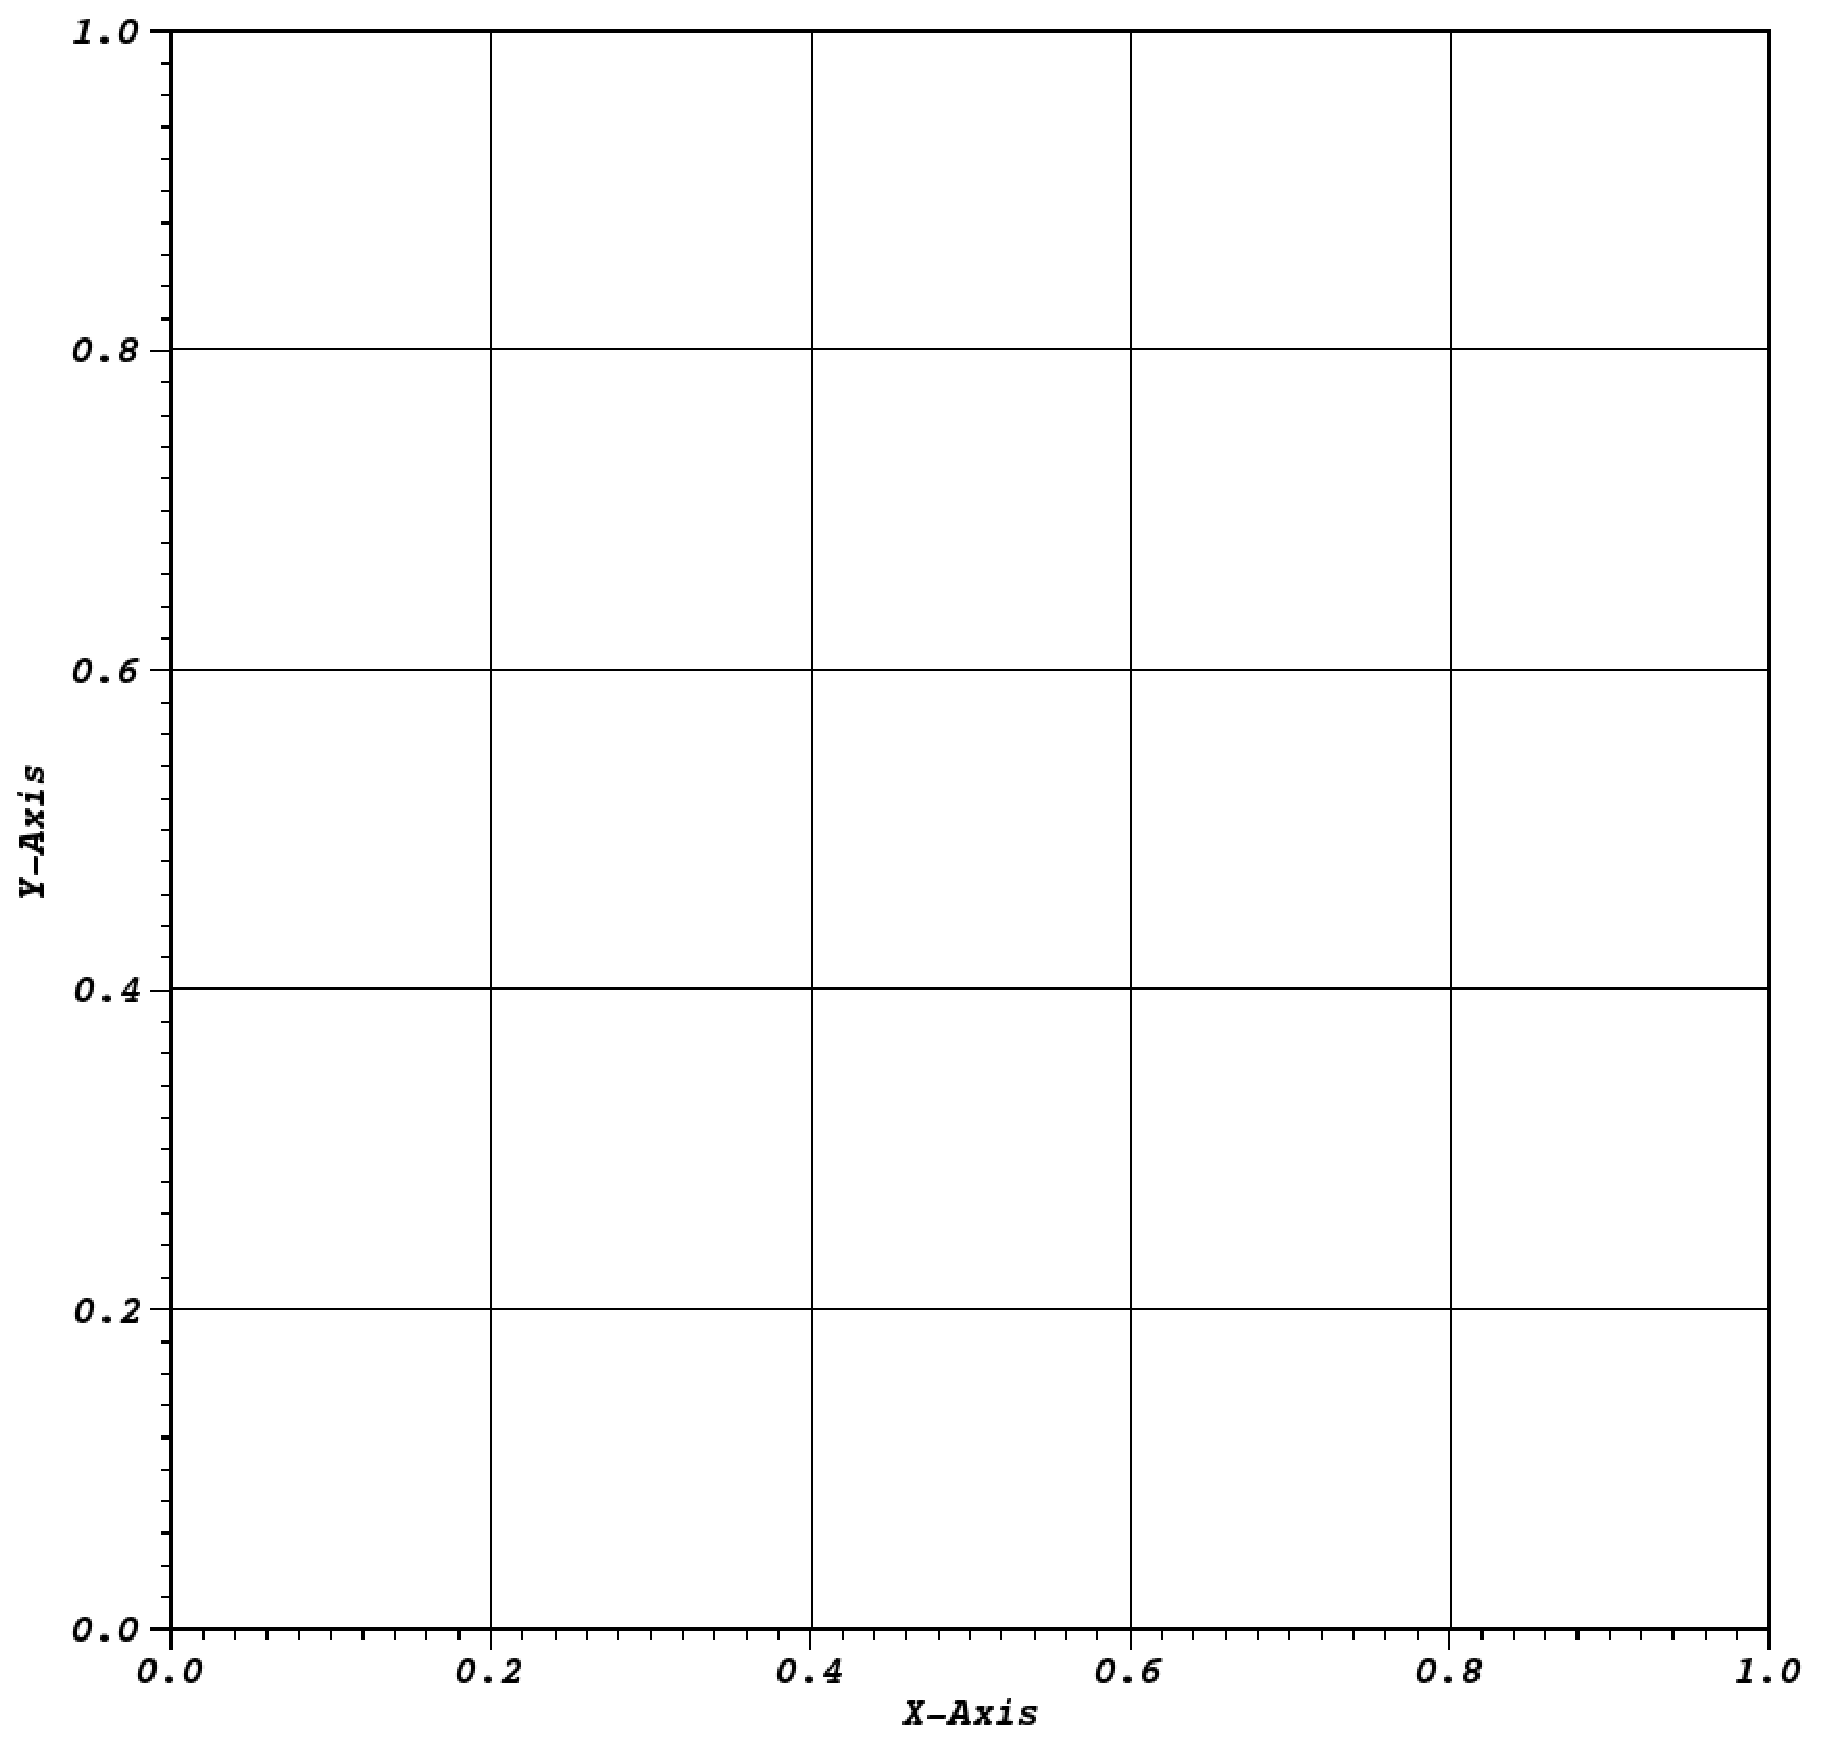
\includegraphics[width=0.45\textwidth]{figures/sec_BF/searchlight_starting_mesh.eps}
\caption{Initial mesh configuration for the searchlight problem before any refinement cycles.}
\label{fig::BF_Results_SL_starting_mesh}
\end{figure}

\begin{figure}
\centering
	\begin{subfigure}[b]{0.45\textwidth}
		\centering
		\label{subfig::SL_uniform_ef_wach}
		\includegraphics[width=\textwidth]{figures/sec_BF/SL_WACHSPRESS_uniform.eps}
		\caption{}
	\end{subfigure}
	\vfill
	\begin{subfigure}[b]{0.45\textwidth}
		\centering
		\label{subfig::SL_uniform_ef_pwld}
		\includegraphics[width=\textwidth]{figures/sec_BF/SL_PWLD_uniform.eps}
		\caption{}
	\end{subfigure}
	\hfill
	\begin{subfigure}[b]{0.45\textwidth}
		\centering
		\label{subfig::SL_uniform_ef_mv}
		\includegraphics[width=\textwidth]{figures/sec_BF/SL_MV_uniform.eps}
		\caption{}
	\end{subfigure}
	\vfill
	\begin{subfigure}[b]{0.45\textwidth}
		\centering
		\label{subfig::SL_uniform_ef_me1}
		\includegraphics[width=\textwidth]{figures/sec_BF/SL_ME_k1_uniform.eps}
		\caption{}
	\end{subfigure}
	\hfill
	\begin{subfigure}[b]{0.45\textwidth}
		\centering
		\label{subfig::SL_uniform_ef_me2}
		\includegraphics[width=\textwidth]{figures/sec_BF/SL_ME_k2_uniform.eps}
		\caption{}
	\end{subfigure}
\caption{Exiting angular flux on the right boundary with uniform refinement using the (a) Wachspress basis functions, (b) PWL basis functions, (c) mean value basis functions, (d) linear maximum entropy coordinates and (e) quadratic serendipity maximum entropy coordinates.}
\label{fig::BF_Results_SL_uniform_exit_flux}
\end{figure}

%%%%%%%%%%%%%%%%%%%%%%%%%%%%%%%%%%%%%%%%%%%%%%%%%%%
%%%   Section - Conclusions
\section{Conclusions}
\label{sec::BF_Conclusions}

In this chapter, we have presented 







